% Options for packages loaded elsewhere
%DIF LATEXDIFF DIFFERENCE FILE
%DIF DEL ms/ms-v1-submitted.tex   Fri Jul 10 08:57:23 2026
%DIF ADD ms/ms.tex                Wed Aug 19 02:07:39 2026
% Options for packages loaded elsewhere
\PassOptionsToPackage{unicode}{hyperref}
\PassOptionsToPackage{hyphens}{url}
\PassOptionsToPackage{dvipsnames,svgnames,x11names}{xcolor}
%
\documentclass[
  letterpaper,
  DIV=11,
  numbers=noendperiod]{scrartcl}
\usepackage{xcolor}
\usepackage{amsmath,amssymb}
\setcounter{secnumdepth}{-\maxdimen} % remove section numbering
\usepackage{iftex}
\ifPDFTeX
  \usepackage[T1]{fontenc}
  \usepackage[utf8]{inputenc}
  \usepackage{textcomp} % provide euro and other symbols
\else % if luatex or xetex
  \usepackage{unicode-math} % this also loads fontspec
  \defaultfontfeatures{Scale=MatchLowercase}
  \defaultfontfeatures[\rmfamily]{Ligatures=TeX,Scale=1}
\fi
\usepackage{lmodern}
\ifPDFTeX\else
  % xetex/luatex font selection
  \setmainfont[]{Times New Roman}
\fi
% Use upquote if available, for straight quotes in verbatim environments
\IfFileExists{upquote.sty}{\usepackage{upquote}}{}
\IfFileExists{microtype.sty}{% use microtype if available
  \usepackage[]{microtype}
  \UseMicrotypeSet[protrusion]{basicmath} % disable protrusion for tt fonts
}{}
% Make \paragraph and \subparagraph free-standing
\makeatletter
\ifx\paragraph\undefined\else
  \let\oldparagraph\paragraph
  \renewcommand{\paragraph}{
    \@ifstar
      \xxxParagraphStar
      \xxxParagraphNoStar
  }
  \newcommand{\xxxParagraphStar}[1]{\oldparagraph*{#1}\mbox{}}
  \newcommand{\xxxParagraphNoStar}[1]{\oldparagraph{#1}\mbox{}}
\fi
\ifx\subparagraph\undefined\else
  \let\oldsubparagraph\subparagraph
  \renewcommand{\subparagraph}{
    \@ifstar
      \xxxSubParagraphStar
      \xxxSubParagraphNoStar
  }
  \newcommand{\xxxSubParagraphStar}[1]{\oldsubparagraph*{#1}\mbox{}}
  \newcommand{\xxxSubParagraphNoStar}[1]{\oldsubparagraph{#1}\mbox{}}
\fi
\makeatother


\usepackage{longtable,booktabs,array}
\newcounter{none} % for unnumbered tables
\usepackage{calc} % for calculating minipage widths
% Correct order of tables after \paragraph or \subparagraph
\usepackage{etoolbox}
\makeatletter
\patchcmd\longtable{\par}{\if@noskipsec\mbox{}\fi\par}{}{}
\makeatother
% Allow footnotes in longtable head/foot
\IfFileExists{footnotehyper.sty}{\usepackage{footnotehyper}}{\usepackage{footnote}}
\makesavenoteenv{longtable}
\usepackage{graphicx}
\makeatletter
\newsavebox\pandoc@box
\newcommand*\pandocbounded[1]{% scales image to fit in text height/width
  \sbox\pandoc@box{#1}%
  \Gscale@div\@tempa{\textheight}{\dimexpr\ht\pandoc@box+\dp\pandoc@box\relax}%
  \Gscale@div\@tempb{\linewidth}{\wd\pandoc@box}%
  \ifdim\@tempb\p@<\@tempa\p@\let\@tempa\@tempb\fi% select the smaller of both
  \ifdim\@tempa\p@<\p@\scalebox{\@tempa}{\usebox\pandoc@box}%
  \else\usebox{\pandoc@box}%
  \fi%
}
% Set default figure placement to htbp
\def\fps@figure{htbp}
\makeatother


% definitions for citeproc citations
\NewDocumentCommand\citeproctext{}{}
\NewDocumentCommand\citeproc{mm}{%
  \begingroup\def\citeproctext{#2}\cite{#1}\endgroup}
\makeatletter
 % allow citations to break across lines
 \let\@cite@ofmt\@firstofone
 % avoid brackets around text for \cite:
 \def\@biblabel#1{}
 \def\@cite#1#2{{#1\if@tempswa , #2\fi}}
\makeatother
\newlength{\cslhangindent}
\setlength{\cslhangindent}{1.5em}
\newlength{\csllabelwidth}
\setlength{\csllabelwidth}{3em}
\newenvironment{CSLReferences}[2] % #1 hanging-indent, #2 entry-spacing
 {\begin{list}{}{%
  \setlength{\itemindent}{0pt}
  \setlength{\leftmargin}{0pt}
  \setlength{\parsep}{0pt}
  % turn on hanging indent if param 1 is 1
  \ifodd #1
   \setlength{\leftmargin}{\cslhangindent}
   \setlength{\itemindent}{-1\cslhangindent}
  \fi
  % set entry spacing
  \setlength{\itemsep}{#2\baselineskip}}}
 {\end{list}}
\usepackage{calc}
\newcommand{\CSLBlock}[1]{\hfill\break\parbox[t]{\linewidth}{\strut\ignorespaces#1\strut}}
\newcommand{\CSLLeftMargin}[1]{\parbox[t]{\csllabelwidth}{\strut#1\strut}}
\newcommand{\CSLRightInline}[1]{\parbox[t]{\linewidth - \csllabelwidth}{\strut#1\strut}}
\newcommand{\CSLIndent}[1]{\hspace{\cslhangindent}#1}



\setlength{\emergencystretch}{3em} % prevent overfull lines

\providecommand{\tightlist}{%
  \setlength{\itemsep}{0pt}\setlength{\parskip}{0pt}}



 


\usepackage{booktabs}
\usepackage{longtable}
\usepackage{array}
\usepackage{multirow}
\usepackage{wrapfig}
\usepackage{float}
\usepackage{colortbl}
\usepackage{pdflscape}
\usepackage{tabu}
\usepackage{threeparttable}
\usepackage{threeparttablex}
\usepackage[normalem]{ulem}
\usepackage{makecell}
\usepackage{xcolor}
\KOMAoption{captions}{tableheading}
\usepackage{hyperref}
\addtokomafont{disposition}{\rmfamily}
\usepackage{siunitx}
%DIF 152-154d152
%DIF < \newcommand{\Aamphi}{$A_{\mathrm{amphi}}$}
%DIF < \newcommand{\Ahypo}{$A_{\mathrm{hypo}}$}
%DIF < \newcommand{\agcurve}{$A \textendash g_\mathrm{sw}$}
%DIF -------
\newcommand{\ca}{$C_\mathrm{a}$}
\newcommand{\caequals}[1]{$C_\mathrm{a} = \SI{#1}{\micro\mol\raiseto{-1}\mol}$}
%DIF 157d154
%DIF < \newcommand{\cabetween}[2]{#1 < $C_\mathrm{a} < \SI{#2}{\micro\mol\raiseto{-1}\mol}$}
%DIF -------
\newcommand{\fgmax}{$f_\mathrm{gmax}$}
\newcommand{\gcl}{$l_\mathrm{gc}$}
%DIF 160a156-157
\newcommand{\gi}{$g_\mathrm{i}$} %DIF > 
\newcommand{\gf}{$g_\mathrm{f}$} %DIF > 
%DIF -------
\newcommand{\gmax}{$g_\mathrm{max}$}
%DIF 161-163d159
%DIF < \newcommand{\gmaxratio}{$g_\mathrm{max,ratio}$}
%DIF < \newcommand{\gmaxshade}{$g_\mathrm{max,shade}$}
%DIF < \newcommand{\gmaxsun}{$g_\mathrm{max,sun}$}
%DIF -------
\newcommand{\gop}{$g_\mathrm{op}$}
\newcommand{\gsw}{$g_\mathrm{sw}$}
%DIF 166-167c161-162
%DIF < \newcommand{\loggsw}{$\log(g_\mathrm{sw})$}
%DIF < \newcommand{\logA}{$\log(A)$}
%DIF -------
\newcommand{\loggi}{$\log(g_\mathrm{i})$} %DIF > 
\newcommand{\loggmax}{$\log(g_\mathrm{max})$} %DIF > 
%DIF -------
\newcommand{\ppfd}{$\mathrm{PPFD}$}
\newcommand{\ppfdequals}[1]{$\mathrm{PPFD} = \SI{#1}{\micro\mole\per\meter\squared\per\second}$}
\newcommand{\ppfdqty}[1]{$\SI{#1}{\micro\mole\per\meter\squared\per\second}$}
\newcommand{\rh}{$\mathrm{RH}$}
\newcommand{\rhequals}[1]{$\mathrm{RH} = #1\%$}
\newcommand{\tleafequals}[1]{$T_\mathrm{leaf} = \SI{#1}{\degreeCelsius}$}
\usepackage{setspace}
\usepackage[modulo]{lineno}
\usepackage{physics}
\usepackage{pifont}
\newcommand{\cmark}{\ding{51}}
\DeclareMathOperator{\logit}{logit}
% To control table and figure placements
\usepackage{placeins}
%DIF 182a177-178
% For multi-line table headers %DIF > 
\usepackage{makecell} %DIF > 
%DIF -------
\makeatletter
\@ifpackageloaded{caption}{}{\usepackage{caption}}
\AtBeginDocument{%
\ifdefined\contentsname
  \renewcommand*\contentsname{Table of contents}
\else
  \newcommand\contentsname{Table of contents}
\fi
\ifdefined\listfigurename
  \renewcommand*\listfigurename{List of Figures}
\else
  \newcommand\listfigurename{List of Figures}
\fi
\ifdefined\listtablename
  \renewcommand*\listtablename{List of Tables}
\else
  \newcommand\listtablename{List of Tables}
\fi
\ifdefined\figurename
  \renewcommand*\figurename{Figure}
\else
  \newcommand\figurename{Figure}
\fi
\ifdefined\tablename
  \renewcommand*\tablename{Table}
\else
  \newcommand\tablename{Table}
\fi
}
\@ifpackageloaded{float}{}{\usepackage{float}}
\floatstyle{ruled}
\@ifundefined{c@chapter}{\newfloat{codelisting}{h}{lop}}{\newfloat{codelisting}{h}{lop}[chapter]}
\floatname{codelisting}{Listing}
\newcommand*\listoflistings{\listof{codelisting}{List of Listings}}
\makeatother
\makeatletter
\makeatother
\makeatletter
\@ifpackageloaded{caption}{}{\usepackage{caption}}
\@ifpackageloaded{subcaption}{}{\usepackage{subcaption}}
\makeatother
\usepackage{bookmark}
\IfFileExists{xurl.sty}{\usepackage{xurl}}{} % add URL line breaks if available
\urlstyle{same}
\hypersetup{
%DIF 227c224
%DIF <   pdftitle={Guard cell size and pore aperture influence stomatal closure kinetics},
%DIF -------
  pdftitle={Guard cell size and initial conductance influence stomatal closure kinetics}, %DIF > 
%DIF -------
  pdfauthor={Christopher D. Muir\^{}\{1,2*\}; Wei Shen Lim\^{}\{1\}},
  colorlinks=true,
  linkcolor={blue},
  filecolor={Maroon},
  citecolor={Blue},
  urlcolor={Blue},
  pdfcreator={LaTeX via pandoc}}


\title{Guard cell size and \DIFdelbegin \DIFdel{pore aperture }\DIFdelend \DIFaddbegin \DIFadd{initial conductance }\DIFaddend influence stomatal
closure kinetics}
\author{Christopher D. Muir\(^{1,2*}\) \and Wei Shen Lim\(^{1}\)}
\date{}
%DIF PREAMBLE EXTENSION ADDED BY LATEXDIFF
%DIF UNDERLINE PREAMBLE %DIF PREAMBLE
\RequirePackage[normalem]{ulem} %DIF PREAMBLE
\RequirePackage{color}\definecolor{RED}{rgb}{1,0,0}\definecolor{BLUE}{rgb}{0,0,1} %DIF PREAMBLE
\providecommand{\DIFaddtex}[1]{{\protect\color{blue}\uwave{#1}}} %DIF PREAMBLE
\providecommand{\DIFdeltex}[1]{{\protect\color{red}\sout{#1}}}                      %DIF PREAMBLE
%DIF SAFE PREAMBLE %DIF PREAMBLE
\providecommand{\DIFaddbegin}{} %DIF PREAMBLE
\providecommand{\DIFaddend}{} %DIF PREAMBLE
\providecommand{\DIFdelbegin}{} %DIF PREAMBLE
\providecommand{\DIFdelend}{} %DIF PREAMBLE
\providecommand{\DIFmodbegin}{} %DIF PREAMBLE
\providecommand{\DIFmodend}{} %DIF PREAMBLE
%DIF FLOATSAFE PREAMBLE %DIF PREAMBLE
\providecommand{\DIFaddFL}[1]{\DIFadd{#1}} %DIF PREAMBLE
\providecommand{\DIFdelFL}[1]{\DIFdel{#1}} %DIF PREAMBLE
\providecommand{\DIFaddbeginFL}{} %DIF PREAMBLE
\providecommand{\DIFaddendFL}{} %DIF PREAMBLE
\providecommand{\DIFdelbeginFL}{} %DIF PREAMBLE
\providecommand{\DIFdelendFL}{} %DIF PREAMBLE
%DIF HYPERREF PREAMBLE %DIF PREAMBLE
\providecommand{\DIFadd}[1]{\texorpdfstring{\DIFaddtex{#1}}{#1}} %DIF PREAMBLE
\providecommand{\DIFdel}[1]{\texorpdfstring{\DIFdeltex{#1}}{}} %DIF PREAMBLE
\newcommand{\DIFscaledelfig}{0.5}
%DIF HIGHLIGHTGRAPHICS PREAMBLE %DIF PREAMBLE
\RequirePackage{settobox} %DIF PREAMBLE
\RequirePackage{letltxmacro} %DIF PREAMBLE
\newsavebox{\DIFdelgraphicsbox} %DIF PREAMBLE
\newlength{\DIFdelgraphicswidth} %DIF PREAMBLE
\newlength{\DIFdelgraphicsheight} %DIF PREAMBLE
% store original definition of \includegraphics %DIF PREAMBLE
\LetLtxMacro{\DIFOincludegraphics}{\includegraphics} %DIF PREAMBLE
\newcommand{\DIFaddincludegraphics}[2][]{{\color{blue}\fbox{\DIFOincludegraphics[#1]{#2}}}} %DIF PREAMBLE
\newcommand{\DIFdelincludegraphics}[2][]{% %DIF PREAMBLE
\sbox{\DIFdelgraphicsbox}{\DIFOincludegraphics[#1]{#2}}% %DIF PREAMBLE
\settoboxwidth{\DIFdelgraphicswidth}{\DIFdelgraphicsbox} %DIF PREAMBLE
\settoboxtotalheight{\DIFdelgraphicsheight}{\DIFdelgraphicsbox} %DIF PREAMBLE
\scalebox{\DIFscaledelfig}{% %DIF PREAMBLE
\parbox[b]{\DIFdelgraphicswidth}{\usebox{\DIFdelgraphicsbox}\\[-\baselineskip] \rule{\DIFdelgraphicswidth}{0em}}\llap{\resizebox{\DIFdelgraphicswidth}{\DIFdelgraphicsheight}{% %DIF PREAMBLE
\setlength{\unitlength}{\DIFdelgraphicswidth}% %DIF PREAMBLE
\begin{picture}(1,1)% %DIF PREAMBLE
\thicklines\linethickness{2pt} %DIF PREAMBLE
{\color[rgb]{1,0,0}\put(0,0){\framebox(1,1){}}}% %DIF PREAMBLE
{\color[rgb]{1,0,0}\put(0,0){\line( 1,1){1}}}% %DIF PREAMBLE
{\color[rgb]{1,0,0}\put(0,1){\line(1,-1){1}}}% %DIF PREAMBLE
\end{picture}% %DIF PREAMBLE
}\hspace*{3pt}}} %DIF PREAMBLE
} %DIF PREAMBLE
\LetLtxMacro{\DIFOaddbegin}{\DIFaddbegin} %DIF PREAMBLE
\LetLtxMacro{\DIFOaddend}{\DIFaddend} %DIF PREAMBLE
\LetLtxMacro{\DIFOdelbegin}{\DIFdelbegin} %DIF PREAMBLE
\LetLtxMacro{\DIFOdelend}{\DIFdelend} %DIF PREAMBLE
\DeclareRobustCommand{\DIFaddbegin}{\DIFOaddbegin \let\includegraphics\DIFaddincludegraphics} %DIF PREAMBLE
\DeclareRobustCommand{\DIFaddend}{\DIFOaddend \let\includegraphics\DIFOincludegraphics} %DIF PREAMBLE
\DeclareRobustCommand{\DIFdelbegin}{\DIFOdelbegin \let\includegraphics\DIFdelincludegraphics} %DIF PREAMBLE
\DeclareRobustCommand{\DIFdelend}{\DIFOaddend \let\includegraphics\DIFOincludegraphics} %DIF PREAMBLE
\LetLtxMacro{\DIFOaddbeginFL}{\DIFaddbeginFL} %DIF PREAMBLE
\LetLtxMacro{\DIFOaddendFL}{\DIFaddendFL} %DIF PREAMBLE
\LetLtxMacro{\DIFOdelbeginFL}{\DIFdelbeginFL} %DIF PREAMBLE
\LetLtxMacro{\DIFOdelendFL}{\DIFdelendFL} %DIF PREAMBLE
\DeclareRobustCommand{\DIFaddbeginFL}{\DIFOaddbeginFL \let\includegraphics\DIFaddincludegraphics} %DIF PREAMBLE
\DeclareRobustCommand{\DIFaddendFL}{\DIFOaddendFL \let\includegraphics\DIFOincludegraphics} %DIF PREAMBLE
\DeclareRobustCommand{\DIFdelbeginFL}{\DIFOdelbeginFL \let\includegraphics\DIFdelincludegraphics} %DIF PREAMBLE
\DeclareRobustCommand{\DIFdelendFL}{\DIFOaddendFL \let\includegraphics\DIFOincludegraphics} %DIF PREAMBLE
%DIF COLORLISTINGS PREAMBLE %DIF PREAMBLE
\RequirePackage{listings} %DIF PREAMBLE
\RequirePackage{color} %DIF PREAMBLE
\lstdefinelanguage{DIFcode}{ %DIF PREAMBLE
%DIF DIFCODE_UNDERLINE %DIF PREAMBLE
  moredelim=[il][\color{red}\sout]{\%DIF\ <\ }, %DIF PREAMBLE
  moredelim=[il][\color{blue}\uwave]{\%DIF\ >\ } %DIF PREAMBLE
} %DIF PREAMBLE
\lstdefinestyle{DIFverbatimstyle}{ %DIF PREAMBLE
	language=DIFcode, %DIF PREAMBLE
	basicstyle=\ttfamily, %DIF PREAMBLE
	columns=fullflexible, %DIF PREAMBLE
	keepspaces=true %DIF PREAMBLE
} %DIF PREAMBLE
\lstnewenvironment{DIFverbatim}{\lstset{style=DIFverbatimstyle}}{} %DIF PREAMBLE
\lstnewenvironment{DIFverbatim*}{\lstset{style=DIFverbatimstyle,showspaces=true}}{} %DIF PREAMBLE
%DIF END PREAMBLE EXTENSION ADDED BY LATEXDIFF

\begin{document}
\maketitle


\begin{center}
$^1$School of Life Sciences, University of Hawaiʻi; Mānoa, Hawaiʻi, USA\\
$^2$Department of Botany, University of Wisconsin, Madison; Wisconsin, USA\\
\medskip
*Corresponding author: cdmuir@wisc.edu\\
\medskip
ORCID: Christopher D. Muir — \href{https://orcid.org/0000-0003-2555-3878}{0000-0003-2555-3878}\\
ORCID: Wei Shen Lim — \href{https://orcid.org/0009-0001-1406-7957}{0009-0001-1406-7957}\\
\medskip
Keywords: \DIFdelbegin \DIFdel{amphistomy}\DIFdelend \DIFaddbegin \DIFadd{guard cell size}\DIFaddend , leaf gas exchange, \DIFaddbegin \DIFadd{phylogenetic heritability, }\DIFaddend \textit{Solanum}, stomatal kinetics, \DIFdelbegin \DIFdel{stomatal size
}\DIFdelend \DIFaddbegin \DIFadd{vapor pressure deficit
}\DIFaddend \end{center}

\linenumbers
% \doublespacing
\onehalfspacing

\newpage{}

\subsection{Summary}\label{summary}

\begin{itemize}
\item
  In fluctuating environments, the kinetics of stomatal opening and
  closing influence the balance between carbon gain and water loss.
  \DIFdelbegin \DIFdel{The
  rate of stomatal aperture change varies widely among plants, but the
  underlying causes of this variation are not well understood. One
  hypothesis is that smaller guard cells }\DIFdelend \DIFaddbegin \DIFadd{Smaller guard cells may }\DIFaddend respond faster to fluctuating environmental
  conditions because of their greater surface area for osmolyte flux
  relative to cell volume. A related hypothesis is that operational
  stomatal conductance (\gop) is often well below its theoretical
  maximum (\gmax) because at this stomatal aperture, guard cell volume
  is poised to change rapidly with small changes in turgor pressure.
\DIFdelbegin \DIFdel{The support for both hypotheses is limited and mixed, in
  part because they have not been tested together.
}\DIFdelend \item
  We analyzed 2,\DIFdelbegin \DIFdel{124 }\DIFdelend \DIFaddbegin \DIFadd{125 }\DIFaddend estimates of stomatal closure kinetics in response
  to an abrupt increase in vapor pressure deficit (VPD) among 29 diverse
  wild tomato populations in the genus \emph{Solanum}.
\item
  \DIFdelbegin \DIFdel{Both smaller guard cell size }\DIFdelend \DIFaddbegin \DIFadd{Leaves with small guard cells }\DIFaddend and a lower \DIFdelbegin \DIFdel{\gop{} to \gmax{} ratio
  (\fgmax) were associated with fasterstomatal closure kinetics, but }\DIFdelend \DIFaddbegin \DIFadd{initial stomatal conductance
  (\gi) closed faster, but each explained variation in kinetic
  parameters }\DIFaddend at different levels of biological organization. Guard cell
  size had high phylogenetic heritability and varied relatively little
  within populations, whereas \DIFdelbegin \DIFdel{\fgmax{} }\DIFdelend \DIFaddbegin \DIFadd{\gi{} }\DIFaddend varied mostly among individuals and
  between light intensity treatments.
\item
  \DIFdelbegin \DIFdel{Together, these results indicate that smaller }\DIFdelend \DIFaddbegin \DIFadd{Smaller }\DIFaddend stomata can be speedier, but \DIFdelbegin \DIFdel{only if stomata are held at an aperture where they are responsive
  to
  changing turgor pressure. We predict that selection }\DIFdelend \DIFaddbegin \DIFadd{the current physiological state
  of the leaf also affects the responsiveness of stomatal conductance to
  fluctuations. Selection }\DIFaddend on stomatal speed \DIFdelbegin \DIFdel{will }\DIFdelend \DIFaddbegin \DIFadd{may }\DIFaddend influence not only
  anatomical traits like guard cell size, but also physiological
  controls on \gop.
\end{itemize}

\newpage{}

\subsection{Introduction}\label{introduction}

In nature, change is the only constant. One way that vascular plants
(tracheophytes) cope with change is by adjusting stomatal pore aperture
to optimize the trade-off between carbon gain and water loss (Cowan \&
Farquhar, 1977; Raven, 2002; Hetherington \& Woodward, 2003). In the
absence of physical limits and energetic tradeoffs, natural selection
would favor plants that could instantaneously adjust stomatal
conductance (\gsw) to perfectly track dynamic environmental conditions
(Lawson \emph{et al.}, 2010). In reality, stomatal responses take time,
creating a lag between actual and optimal stomatal aperture. For
example, many species use hydroactive feedback mechanisms to precisely
control stomatal responses to changing vapor pressure deficit (VPD), the
driving force for evaporation (Buckley, 2019)\DIFdelbegin \DIFdel{. Hydroactive stomatal
control
requires sensing }\DIFdelend \DIFaddbegin \DIFadd{, but hydroactive control
takes time. Leaves must sense }\DIFaddend a change in VPD through as-yet-unknown
mechanisms \DIFdelbegin \DIFdel{, signal transduction, and }\DIFdelend \DIFaddbegin \DIFadd{and then transduce a signal that causes }\DIFaddend efflux of osmotic
solutes to alter guard cell turgor more than the surrounding epidermal
cells. Abscisic acid (ABA) dependent responses require several minutes
to accumulate or synthesize hormone pools \emph{de novo} (Xie \emph{et
al.}, 2006; Bauer \emph{et al.}, 2013; McAdam \emph{et al.}, 2016; Desai
\& Stroock, 2025\DIFaddbegin \DIFadd{; Pichaco }\emph{\DIFadd{et al.}}\DIFadd{, 2026}\DIFaddend ); ABA-independent stomatal
responses require changes in gene expression and protein synthesis that
take time (Jalakas \emph{et al.}, 2021). Once anion channels are
activated, the rate of change in stomatal aperture depends on the rate
of change in guard cell turgor (\(d P_\mathrm{g} / dt\)) and the
sensitivity of aperture to change in turgor
(\(d a_\mathrm{S} / d P_\mathrm{g}\)). As we discuss below, these two
factors (\(d P_\mathrm{g} / dt\) and
\(d a_\mathrm{S} / d P_\mathrm{g}\)) may be influenced by guard cell
size and the ratio of operational to maximum stomatal conductance
(\fgmax), respectively.

Over a century ago Darwin (1898) observed that after an initial
increase, leaf transpiration decreases in response to decreasing
humidity. He correctly attributed changes in transpiration to changes in
stomatal aperture and subsequent studies have confirmed that stomatal
aperture responds to humidity (Lange \emph{et al.}, 1971) and, more
specifically, transpiration rate (Mott \& Parkhurst, 1991; Monteith,
1995), which is the product of VPD and \gsw. The VPD is related to
relative humidity (RH) but also temperature. In angiosperms and some
pteridophytes, a sudden increase in VPD, usually induced by lower RH at
a constant temperature, causes a transient increase in \gsw, as Darwin
observed (Cowan, 1972; Buckley \emph{et al.}, 2011; Westbrook \& McAdam,
2021). After a period of several minutes, stomata close until the leaf
reaches a new steady-state \gsw. These phases of stomatal response to
VPD are often referred to as the ``wrong-way response'' (WWR) and
``right-way response'' (RWR), respectively. The normative `wrong' and
`right' appellations refer to the presumed adaptive significance. At
steady state, \gsw{} is negatively correlated with VPD, all else being
equal, which is interpreted as an adaptive response to the marginal
carbon cost of water (Givnish \& Vermeij, 1976; Cowan \& Farquhar, 1977;
Buckley \emph{et al.}, 2017b). Models built around this assumption
generally predict steady state \gsw{} well, although the functional form
and presumed fitness costs are areas of active research (Damour \emph{et
al.}, 2010; Medlyn \emph{et al.}, 2011; Prentice \emph{et al.}, 2014;
Sperry \emph{et al.}, 2017; Potkay \emph{et al.}, 2025).

Stomatal responses are as much about the journey (kinetics) as they are
about the destination (steady state). If stomatal response kinetics are
too slow relative to the temporal grain size of environmental
variability, then it would be futile for \gsw{} to track environmental
variation since the leaf will constantly lag the environment,
perpetually fighting the last war. This may explain why \gsw{} can be
insensitive to short sun/shade flecks (Knapp \& Smith, 1990) and shaded
leaves are likely primed to cope with the hydraulic demands of sudden
increases in light, temperature, and VPD (Schymanski \emph{et al.},
2013). If stomatal responses can track environmental variation, then
minimizing the lag time can greatly improve resource-use efficiency
(Lawson \emph{et al.}, 2010). For example, optogenetic control of
stomatal aperture in response to fluctuating light increases water-use
efficiency in \emph{Arabidopsis} compared to wild-type responses
(Papanatsiou \emph{et al.}, 2019). Therefore the rate of stomatal
opening and closing is predicted to have a major effect on how natural
selection optimizes stomatal control in variable environments (Buckley
\emph{et al.}, 2023).

Much of the research on stomatal kinetics focuses on light responses
because light intensity is usually the most important, rapidly
fluctuating environmental variable affecting photosynthesis. In nature,
fluctuating light intensity \DIFdelbegin \DIFdel{simulataneously }\DIFdelend \DIFaddbegin \DIFadd{simultaneously }\DIFaddend alters leaf temperature and
VPD (e.g. Ishida \emph{et al.}, 1992). We focus on stomatal closure
kinetics in response to an abrupt \DIFdelbegin \DIFdel{increased in VPD}\DIFdelend \DIFaddbegin \DIFadd{increase in VPD, rather than light,
}\DIFaddend for four reasons. First of all, the primary aims and \emph{a priori}
hypotheses of this study were not to study stomatal kinetic parameters
and are described in Muir \emph{et al.} (2025). The idea to
opportunistically use \gsw-response curves \DIFdelbegin \DIFdel{generated during this study to test hypotheses
about which traits influence }\DIFdelend \DIFaddbegin \DIFadd{to study }\DIFaddend stomatal kinetics
came after the data had been collected, but not yet analyzed for this
purpose. Second, VPD responses exhibit a similar functional form as
light-responses, suggesting similar underlying mechanisms (Buckley,
2019). Factors that affect stomatal response kinetics to VPD likely
generalize to other environmental variables. Third, humidity responses
tend to dominate over and are faster than other environmental responses
(Aasamaa \& Sõber, 2011a,b), \DIFdelbegin \DIFdel{but }\DIFdelend \DIFaddbegin \DIFadd{although }\DIFaddend there is variation among species
(Merilo \emph{et al.}, 2014). Thus, factors that constrain maximum rates
of stomatal closure are most likely to be observed in response to VPD.
Finally, the ecological salience of VPD responses is increasing as
climate change warms the atmosphere (Grossiord \emph{et al.}, 2020).

Fully describing stomatal responses to the environment is complex
(Buckley \emph{et al.}, 2003; Jezek \emph{et al.}, 2021; Desai \&
Stroock, 2025), but the dynamics of \gsw{} in response to an abrupt
environmental change is well described by relatively simple
phenomenological functions (Vico \emph{et al.}, 2011; McAusland \emph{et
al.}, 2016). A four-parameter equation describes stomatal response
kinetics to a step change in light intensity across dozens of plant
species (Woning \emph{et al.}, 2026):

\begin{equation}\protect\phantomsection\label{eq-weibull}{
  g_\mathrm{sw,t} = g_\mathrm{f} + (g_\mathrm{i} - g_\mathrm{f}) e^{-\left(\frac{t}{\tau}\right)^\lambda}.
}\end{equation}

In this equation, \(g_\mathrm{sw,t}\) is stomatal conductance at time
\(t\), \DIFdelbegin \DIFdel{\(g_\mathrm{i}\) }\DIFdelend \DIFaddbegin \DIFadd{\gi{} }\DIFaddend is the initial \gsw{} before the step change, \DIFdelbegin \DIFdel{\(g_\mathrm{f}\) }\DIFdelend \DIFaddbegin \DIFadd{\gf{} }\DIFaddend is the
final \gsw{} after the step change, \(\tau\) is a time constant that
describes how quickly stomata respond to the step change, and
\(\lambda\) is a shape parameter that describes how the response rate
changes over time. When \(\lambda = 1\), the response rate is constant
over time and \(\tau\) represents the time required for \gsw{} to reach
36.8\% (\(1/e\)) of the way between initial and final values. When
\(\lambda > 1\), the response rate increases over time, and when
\(\lambda < 1\), the response rate decreases over time. Woning \emph{et
al.} (2026) refer to \(\lambda\) as a lag-time parameter because
empirically \(\lambda > 1\). We refer to stomatal kinetic parameters
\(\tau\) (\DIFdelbegin \DIFdel{time-constant}\DIFdelend \DIFaddbegin \DIFadd{time constant}\DIFaddend ) and \(\lambda\) (\DIFdelbegin \DIFdel{lag-time}\DIFdelend \DIFaddbegin \DIFadd{lag time}\DIFaddend ) henceforth. The
first goal of this study is to evaluate whether kinetics of the RWR
after a step change in VPD are adequately described by
Equation~\ref{eq-weibull}. If so, it suggests that some fundamentally
similar mechanisms are shared between light and hydroactive stomatal
responses (Grantz \& Zeiger, 1986).

The main goal of this study is to test hypotheses about which stomatal
anatomical traits affect kinetic parameters \(\tau\) and \(\lambda\). We
consider two interconnected hypotheses that have thus far been treated
in isolation. The first hypothesis is that smaller guard cells open and
close faster because of their intrinsically greater surface area to
volume ratio (Franks \& Farquhar, 2007; Drake \emph{et al.}, 2013;
Lawson \& Vialet-Chabrand, 2019; Woning \emph{et al.}, 2026). For
approximately cylindrical cell geometries, like that found in guard
cells, surface area increases linearly with radius, whereas volume
increases in proportion to the radius squared. Consequently, larger
guard cells will require more time, all else being equal, to achieve a
given change in turgor pressure and, hence, stomatal pore aperture. A
plant with large guard cells can partially compensate for this geometric
constraint by increasing the activity and/or density of ion and solute
transporters in the guard cell plasma membrane (Homann \& Thiel, 2002;
Lawson \& Blatt, 2014; Raven, 2014). However, compensation may be
limited by the available membrane area and/or energetic costs of
maintaining high transporter densities (Vico \emph{et al.}, 2011).
Empirical support for the hypothesis that smaller guard cells are faster
is mixed and has primarily come from step changes in light (Drake
\emph{et al.}, 2013; Elliott-Kingston \emph{et al.}, 2016; McAusland
\emph{et al.}, 2016; Kardiman \& Ræbild, 2018; Haworth \emph{et al.},
2023; \DIFaddbegin \DIFadd{Yoshiyama }\emph{\DIFadd{et al.}}\DIFadd{, 2024; }\DIFaddend Brench \emph{et al.}, 2026; Tang
\emph{et al.}, 2026). Meta-analysis of dozens of species suggests that
stomatal size alone is weakly related to kinetics and modulated by guard
cell shape (Woning \emph{et al.}, 2026). The relationship between guard
cell size and stomatal response kinetics to leaf water potential
(Aasamaa \emph{et al.}, 2001) and VPD (Kübarsepp \emph{et al.}, 2020;
Qie \emph{et al.}, 2024) is less well studied, but similarly equivocal.

One factor that might complicate the relationship between size and speed
is aperture. Stomatal aperture can vary from near 0 when guard cell
turgor pressure is low and asymptotically approach \gmax{} as guard cell
turgor pressure approaches \(\infty\) (Figure~\ref{fig-conceptual}\DIFdelbegin \DIFdel{D}\DIFdelend \DIFaddbegin \DIFadd{d}\DIFaddend ).
The relationship between guard cell turgor pressure and stomatal
aperture is nonlinear (Franks \& Farquhar, 2001) as cell walls become
less elastic at greater turgor (Franks \emph{et al.}, 2001). The
nonlinear relationship between guard cell turgor and pore aperture
implies that if the rate of turgor change is constant
(\(\dv{P}{t} = C\)), the rate of change in aperture, and hence stomatal
conductance, will vary depending on the initial aperture (\(a_0\))
relative to the maximum aperture (\(a_\mathrm{max}\)). Hence,
\(\dv{a}{t} = f(a_0 / a_\mathrm{max})\). When initial aperture is high,
\gsw{} will respond more slowly than when initial aperture is low. Since
we generally do not observe individual stomatal aperture, relating this
idea to leaf-level \gsw{} requires scaling by stomatal density,
biophysical constants, and morphological constants (e.g. Sack \&
Buckley, 2016). We will use the term ``fraction of anatomical maximum
stomatal conductance'', symbolized as \fgmax{} (this is denoted as
\(g_\mathrm{ratio}\) by Xie \emph{et al.} (2022)). This value should be
proportional to the average aperture divided by its maximum aperture for
any arbitrary stomatal density. Leaves operating at \fgmax{} closer to
unity will, all else being equal, be slower to respond than leaves
operating with a \fgmax{} close to zero, independent of stomatal
density. Franks \emph{et al.} (2012) hypothesized that selection on
stomatal density would maintain typical operational stomatal conductance
(\gop) relative to \gmax{} at a sufficiently low value that \gsw{} would
be sensitive to relatively small changes in guard cell turgor pressure.
Consistent with this hypothesis, the \gop:\gmax{} ratio is often near
0.25 (McElwain \emph{et al.}, 2016; Murray \emph{et al.}, 2020), well
below \(f_\mathrm{gmax} = 1\), and in a range where \gsw{} would be
responsive to small changes in guard cell turgor pressure. There is
likely variation within and among species and growth forms in the
\gop:\gmax{} ratio (Xie \emph{et al.}, 2022; Ochoa \emph{et al.}, 2024).

\begin{figure}

\centering{

\pandocbounded{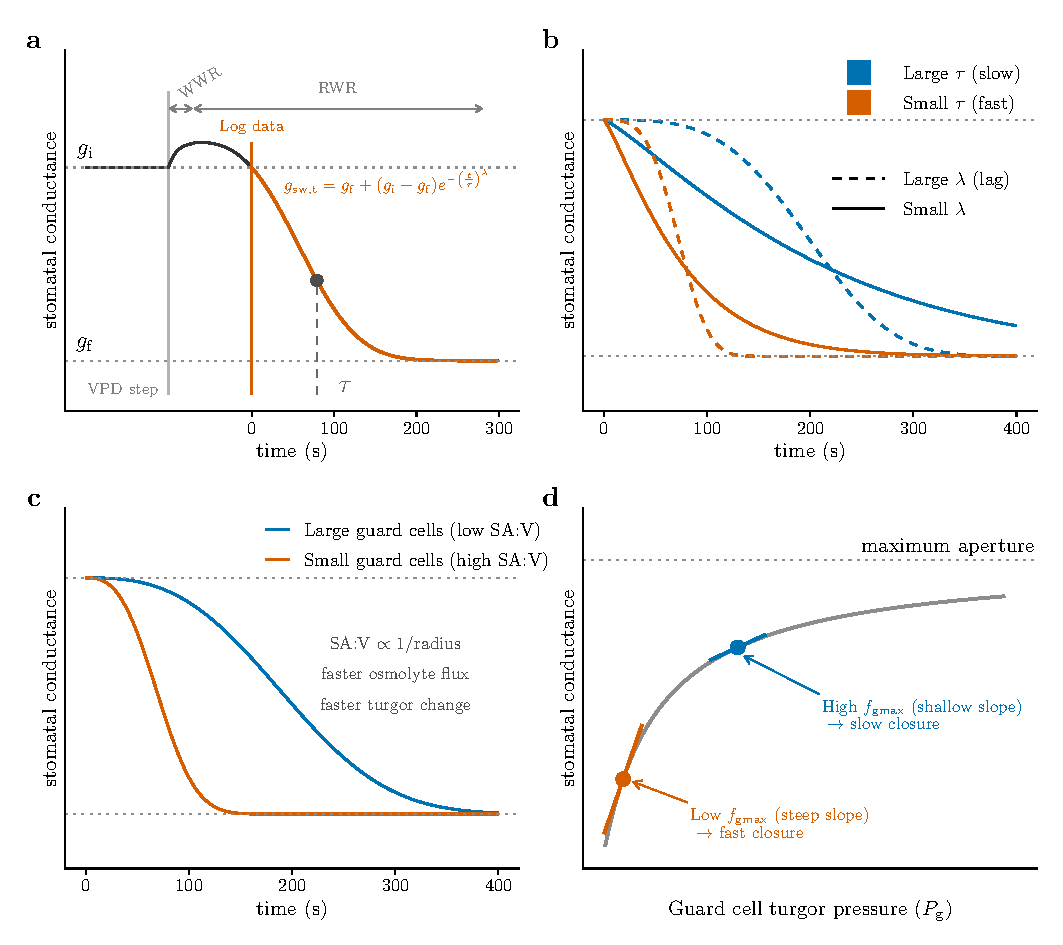
\includegraphics[keepaspectratio]{../figures/conceptual.pdf}}

}

\caption{\label{fig-conceptual}\textbf{Conceptual overview of the two hypotheses linking stomatal anatomy to closure kinetics.}
\DIFdelbeginFL \DIFdelFL{(A) }\DIFdelendFL \DIFaddbeginFL \textbf{\DIFaddFL{a.}} \DIFaddendFL Stomatal conductance (\gsw) in response to a step increase
in vapor pressure deficit (VPD) typically exhibits a transient wrong-way
response (WWR), in which \gsw{} briefly rises, followed by the right-way
response (RWR), in which \gsw{} declines to a lower steady state. The
RWR is well described by a Weibull function (dashed line;
Equation~\ref{eq-weibull}) with initial conductance \(g_\mathrm{i}\),
final conductance \(g_\mathrm{f}\), and kinetic parameters \(\tau\) and
\(\lambda\). \DIFdelbeginFL \DIFdelFL{(B)
}\DIFdelendFL \DIFaddbeginFL \textbf{\DIFaddFL{b.}} \DIFaddendFL The time constant \(\tau\) sets the overall
speed of closure, and the \DIFdelbeginFL \DIFdelFL{lag-time }\DIFdelendFL \DIFaddbeginFL \DIFaddFL{lag time }\DIFaddendFL \(\lambda\) determines whether the
response rate is roughly constant (\(\lambda \approx 1\); solid) or
accelerates over time (\(\lambda > 1\); dashed). \DIFdelbeginFL \DIFdelFL{(C) }\DIFdelendFL \DIFaddbeginFL \textbf{\DIFaddFL{c.}} \DIFaddendFL Smaller
guard cells have a greater surface area to volume ratio (SA:V; schematic
cross-sections shown at right) and are predicted to exchange osmolytes
more quickly across the plasma membrane, yielding a faster change in
guard cell turgor pressure and faster closure. \DIFdelbeginFL \DIFdelFL{(D) }\DIFdelendFL \DIFaddbeginFL \textbf{\DIFaddFL{d.}} \DIFaddendFL The
relationship between guard cell turgor pressure (\(P_g\)) and \gsw{} is
nonlinear and saturating because guard cell walls become less elastic at
higher turgor (Franks \& Farquhar, 2001; Franks \emph{et al.}, 2001).
Consequently, the same change in turgor pressure \DIFdelbeginFL \DIFdelFL{(\(\Delta P_g\), double-headed arrows) }\DIFdelendFL produces a larger
change in \gsw{} when stomata are at low \fgmax{} (\DIFdelbeginFL \DIFdelFL{blue}\DIFdelendFL \DIFaddbeginFL \DIFaddFL{orange}\DIFaddendFL ; steep tangent
slope) than at high \fgmax{} (\DIFdelbeginFL \DIFdelFL{orange}\DIFdelendFL \DIFaddbeginFL \DIFaddFL{blue}\DIFaddendFL ; shallow tangent slope), predicting
slower closure when \fgmax{} is high.}

\end{figure}%

Putting these two hypotheses together, we predict that both guard cell
size and \fgmax{} will influence stomatal kinetics, but possibly at
different scales of biological organization. Guard cell size tends to
vary less than stomatal density or aperture at many biological scales.
For example, on a mature leaf, guard cell length is nearly constant even
as cell volume and pore aperture change with turgor (Willmer \& Fricker,
1996; Franks \emph{et al.}, 2001). Compared to stomatal density, guard
cell size can be less variable (Lammertsma \emph{et al.}, 2011; Bucher
\emph{et al.}, 2016) and evolve more slowly between species (Muir
\emph{et al.}, 2023). If there is relatively little plastic or genetic
variation among individuals within a species, then most of the variance
in stomatal kinetics within species cannot be explained by variation in
guard cell size. In contrast, \fgmax{} can vary immensely within and
among individuals because stomatal aperture responds dynamically over
the day and in response to environmental variation. Because guard cell
size and aperture typically vary at different levels of biological
organization, we predict that guard cell size likely explains more
variation in stomatal kinetics among species, whereas \fgmax{} will
explain more variation within species. Within species variation can
arise from either genetic differences among individuals or environmental
plasticity. We will also test if adaxial stomata respond faster than
abaxial stomata (Haworth \emph{et al.}, 2018; Wall \emph{et al.}, 2022;
Woning \emph{et al.}, 2026) and, if so, whether this difference can be
explained by variation in guard cell size and/or \fgmax{} between
surfaces.

One challenge in determining whether traits covary at higher levels of
organization is that statistical procedures to account for phylogenetic
nonindependence can obscure ecologically relevant covariation caused by
natural selection (Westoby \emph{et al.}, 1995; Uyeda \emph{et al.},
2018). For example, in a meta-analysis of stomatal kinetic responses to
light, the explanatory power of traits like guard cell size and stomatal
ratio declined in phylogenetic compared to nonphylogenetic regression
(Woning \emph{et al.}, 2026). This finding may be caused in large part
because grasses have small stomata, high adaxial:abaxial stomatal ratio,
and rapid stomatal kinetics. Are these associations a coincidence caused
by shared ancestry or ecologically important covariation that helps
explain how grasses adapt to their environment? Recent advances in
phylogenetic comparative methods use hierarchical, multiresponse
phylogenetic models (Muir \emph{et al.}, 2023; Westoby \emph{et al.},
2023; Halliwell \emph{et al.}, 2025) to tease apart ``conservative trait
correlations'' that act at higher levels of organization (e.g.~among
species) from trait correlations that explain variation at lower levels
of organization (e.g.~among individuals within species and plastic
responses). We use this approach to test whether guard cell size and
\fgmax{} explain variation in stomatal kinetics at different levels of
biological organization. Throughout, we use guard cell length (\gcl) as
a proxy for size (Sack \& Buckley, 2016).

The four main questions we address in this study are:

\begin{enumerate}
\def\labelenumi{\arabic{enumi}.}
\tightlist
\item
  Are VPD kinetics adequately characterized by the same functional form
  in Equation~\ref{eq-weibull} as light responses?
\item
  Are \gcl{} and \fgmax{} positively associated with \(\tau\)?
\item
  At what biological levels of organization do \gcl{} and \fgmax{} vary
  and influence \(\tau\)?
\item
  Are abaxial-only stomatal responses slower than whole leaf stomatal
  responses?
\end{enumerate}

As noted above, we are opportunistically analyzing data from an
experiment designed to answer different questions. Before analyzing the
kinetic data, we planned to test whether 1) guard cell size would
influence \(\tau\) and 2) that \(\tau\) would be greater on the
abaxial-only leaves based on a recent meta-analysis of stomatal
responses to light (Woning \emph{et al.}, 2026). We made the decision to
test for an association between \fgmax{} and \(\tau\) after exploratory
analyses revealed a potential association. Adding hypotheses after some
results have been analyzed, also known as ``Hypothesizing After Results
Known'' (HARKing), can lead to reports of spurious associations that are
not repeatable in later studies (Kerr, 1998; Smaldino \& McElreath,
2016). Therefore, our conclusions about the effect of \fgmax{} on
stomatal kinetics should be interpreted with caution until they are
replicated.

\subsection{Materials and Methods}\label{sec-methods}

\subsubsection{Populations and
phylogeny}\label{populations-and-phylogeny}

We grew 29 populations of wild tomato (Table~\ref{tbl-populations}),
including representatives of all described species of \emph{Solanum}
sect. \emph{Lycopersicon} and sect. \emph{Lycopersicoides} (Peralta
\emph{et al.}, 2008), as described in Muir \emph{et al.} (2025). These
populations were selected because they encompass the breadth of climatic
variation in the wild tomato clade (Pease \emph{et al.}, 2016). \DIFdelbegin \DIFdel{In one
case, we substituted a congeneric population of the species (}\emph{\DIFdel{S.
galapagense}}%DIFAUXCMD
\DIFdel{) and added a population of }\emph{\DIFdel{S. pennellii}}%DIFAUXCMD
\DIFdel{. }\DIFdelend Due to
constraints on growth space and time, we spread out measurements over
61.1 weeks\DIFdelbegin \DIFdel{from August 29, 2022 to October 31, 2023. }\DIFdelend \DIFaddbegin \DIFadd{. }\DIFaddend Replicates within population were evenly spread out over
this period to prevent confounding of temporal variation in growth
conditions with variation among populations. \DIFdelbegin \DIFdel{To estimate phylogenetic
effects}\DIFdelend \DIFaddbegin \DIFadd{For phylogenetic
comparative analyses}\DIFaddend , we used the RAxML whole-transcriptome concatenated
phylogeny based on 2,745 100-kb genomic windows from Pease \emph{et al.}
(2016). Two of our populations were not in this tree. We used \emph{S.
galapagense} accession LA1044 in place of LA3909. \emph{S. pennellii}
accession LA0750 was added as sister to LA0716. The node separating
LA0750 from LA0716 was placed \DIFdelbegin \DIFdel{half-way
between the }\DIFdelend \DIFaddbegin \DIFadd{halfway along the branch to the }\DIFaddend next
deepest node.

\DIFdelbegin %DIFDELCMD < \begingroup
%DIFDELCMD < \singlespacing
%DIFDELCMD < 

%DIFDELCMD < \begin{longtable}{>{\raggedright\arraybackslash}p{3.25cm}lrrr}
%DIFDELCMD < 

%DIFDELCMD < \caption{\label{tbl-populations}Accession information of \emph{Solanum}
%DIFDELCMD < populations used in this study. The species name, accession number,
%DIFDELCMD < collection latitude, longitude, and elevation. TGRC: Tomato Genetics
%DIFDELCMD < Resource Center; mas: meters above sea level.}
%DIFDELCMD < 

%DIFDELCMD < \tabularnewline
%DIFDELCMD < 

%DIFDELCMD < \toprule
%DIFDELCMD < Species & TGRC accession & Latitude & Longitude & Elevation (mas)\\
%DIFDELCMD < \midrule
%DIFDELCMD < \endfirsthead
%DIFDELCMD < \multicolumn{5}{@{}l}{\textit{(continued)}}\\
%DIFDELCMD < \toprule
%DIFDELCMD < Species & TGRC accession & Latitude & Longitude & Elevation (mas)\\
%DIFDELCMD < \midrule
%DIFDELCMD < \endhead
%DIFDELCMD < 

%DIFDELCMD < \endfoot
%DIFDELCMD < \bottomrule
%DIFDELCMD < \endlastfoot
%DIFDELCMD < \em{\cellcolor{gray!10}{S. arcanum}} & \cellcolor{gray!10}{LA2172} & \cellcolor{gray!10}{-6.008} & \cellcolor{gray!10}{-78.858} & \cellcolor{gray!10}{662}\\
%DIFDELCMD < \em{S. cheesmaniae} & LA0429 & -0.644 & -90.329 & 800\\
%DIFDELCMD < \em{\cellcolor{gray!10}{S. cheesmaniae}} & \cellcolor{gray!10}{LA3124} & \cellcolor{gray!10}{-0.804} & \cellcolor{gray!10}{-90.042} & \cellcolor{gray!10}{1}\\
%DIFDELCMD < \em{S. chilense} & LA1782 & -15.267 & -74.633 & 1000\\
%DIFDELCMD < \em{\cellcolor{gray!10}{S. chilense}} & \cellcolor{gray!10}{LA4117A} & \cellcolor{gray!10}{-22.907} & \cellcolor{gray!10}{-67.941} & \cellcolor{gray!10}{3540}\\
%DIFDELCMD < \addlinespace
%DIFDELCMD < \em{S. chmielewskii} & LA1028 & -13.883 & -73.017 & 3000\\
%DIFDELCMD < \em{\cellcolor{gray!10}{S. chmielewskii}} & \cellcolor{gray!10}{LA1316} & \cellcolor{gray!10}{-13.400} & \cellcolor{gray!10}{-73.906} & \cellcolor{gray!10}{2920}\\
%DIFDELCMD < \em{S. corneliomulleri} & LA0107 & -13.117 & -76.383 & 60\\
%DIFDELCMD < \em{\cellcolor{gray!10}{S. corneliomulleri}} & \cellcolor{gray!10}{LA0444} & \cellcolor{gray!10}{-13.433} & \cellcolor{gray!10}{-76.133} & \cellcolor{gray!10}{100}\\
%DIFDELCMD < \em{S. galapagense} & LA0436 & -0.953 & -90.978 & 40\\
%DIFDELCMD < \addlinespace
%DIFDELCMD < \em{\cellcolor{gray!10}{S. galapagense}} & \cellcolor{gray!10}{LA1044} & \cellcolor{gray!10}{-0.284} & \cellcolor{gray!10}{-90.548} & \cellcolor{gray!10}{0}\\
%DIFDELCMD < \em{S. habrochaites} & LA0407 & -2.181 & -79.884 & 70\\
%DIFDELCMD < \em{\cellcolor{gray!10}{S. habrochaites}} & \cellcolor{gray!10}{LA1777} & \cellcolor{gray!10}{-9.550} & \cellcolor{gray!10}{-77.700} & \cellcolor{gray!10}{3216}\\
%DIFDELCMD < \em{S. huaylasense} & LA1358 & -9.533 & -77.967 & 750\\
%DIFDELCMD < \em{\cellcolor{gray!10}{S. huaylasense}} & \cellcolor{gray!10}{LA1360} & \cellcolor{gray!10}{-9.546} & \cellcolor{gray!10}{-77.929} & \cellcolor{gray!10}{1490}\\
%DIFDELCMD < \addlinespace
%DIFDELCMD < \em{S. huaylasense} & LA1364 & -10.133 & -77.383 & 2920\\
%DIFDELCMD < \em{\cellcolor{gray!10}{S. lycopersicoides}} & \cellcolor{gray!10}{LA2951} & \cellcolor{gray!10}{-19.317} & \cellcolor{gray!10}{-69.450} & \cellcolor{gray!10}{2200}\\
%DIFDELCMD < \em{S. lycopersicoides} & LA4126 & -19.287 & -69.396 & 3120\\
%DIFDELCMD < \em{\cellcolor{gray!10}{S. neorickii}} & \cellcolor{gray!10}{LA1322} & \cellcolor{gray!10}{-13.483} & \cellcolor{gray!10}{-72.442} & \cellcolor{gray!10}{2380}\\
%DIFDELCMD < \em{S. neorickii} & LA2133 & -3.400 & -79.183 & 1980\\
%DIFDELCMD < \addlinespace
%DIFDELCMD < \em{\cellcolor{gray!10}{S. pennellii}} & \cellcolor{gray!10}{LA0716} & \cellcolor{gray!10}{-16.225} & \cellcolor{gray!10}{-73.617} & \cellcolor{gray!10}{50}\\
%DIFDELCMD < \em{S. pennellii} & LA0750 & -14.775 & -75.034 & 550\\
%DIFDELCMD < \em{\cellcolor{gray!10}{S. pennellii}} & \cellcolor{gray!10}{LA3778} & \cellcolor{gray!10}{-14.775} & \cellcolor{gray!10}{-75.034} & \cellcolor{gray!10}{616}\\
%DIFDELCMD < \em{S. peruvianum} & LA2744 & -18.550 & -70.150 & 400\\
%DIFDELCMD < \em{\cellcolor{gray!10}{S. peruvianum}} & \cellcolor{gray!10}{LA2964} & \cellcolor{gray!10}{-18.028} & \cellcolor{gray!10}{-70.835} & \cellcolor{gray!10}{75}\\
%DIFDELCMD < \addlinespace
%DIFDELCMD < \em{S. pimpinellifolium} & LA1269 & -11.483 & -77.075 & 400\\
%DIFDELCMD < \em{\cellcolor{gray!10}{S. pimpinellifolium}} & \cellcolor{gray!10}{LA1589} & \cellcolor{gray!10}{-8.433} & \cellcolor{gray!10}{-78.817} & \cellcolor{gray!10}{30}\\
%DIFDELCMD < \em{S. pimpinellifolium} & LA2933 & -1.442 & -80.562 & 375\\
%DIFDELCMD < \em{\cellcolor{gray!10}{S. sitiens}} & \cellcolor{gray!10}{LA4116} & \cellcolor{gray!10}{-22.159} & \cellcolor{gray!10}{-68.782} & \cellcolor{gray!10}{2960}\\*
%DIFDELCMD < 

%DIFDELCMD < \end{longtable}
%DIFDELCMD < 

%DIFDELCMD < \endgroup
%DIFDELCMD < 

%DIFDELCMD < %%%
\DIFdelend \subsubsection{Plant growth conditions and light
treatments}\label{plant-growth-conditions-and-light-treatments}

A thorough description of plant growth conditions can be found in Muir
\emph{et al.} (2025), therefore we summarize the most important
information here. Seeds provided by the Tomato Genetics Resource Center
germinated on moist paper in plastic boxes after soaking for 30-60
minutes in a 50\% (volume per volume) solution of household bleach and
water, followed by a thorough rinse. We transferred seedlings to
cell-pack flats containing Pro-Mix BX potting mix (Premier Tech,
Rivière-du-Loup, Quebec, Canada) once cotyledons fully emerged,
typically within 1-2 weeks of sowing. We grew seeds and seedlings for
both sun and shade treatments under the same environmental conditions
(12:12 h, 24.3:\(\SI{21.7}{\degreeCelsius}\), 49.6:58.4 RH day:night
cycle). LED light provided
\(\mathrm{PPFD} = \SI{267}{\micro\mole\per\meter\squared\per\second}\)
(Fluence RAZRx, Austin, Texas, USA) during the germination and seedling
stages.

Immediately prior to starting growth light intensity treatments (sun and
shade), we transplanted seedlings to 3.78 L plastic pots containing 60\%
Pro-Mix BX potting mix, 20\% coral sand (Pro-Pak, Honolulu, Hawaiʻi,
USA), and 20\% cinders (Niu Nursery, Honolulu, Hawaiʻi, USA) with slow
release NPK fertilizer following manufacturer instructions (Osmocote
Smart-Release Plant Food Flower \& Vegetable, The Scotts Company,
Marysville, Ohio, USA). Percentage composition is on a volume basis. We
watered to field capacity three times per week to prevent drought
stress. Seedlings were randomly assigned in alternating order within
population to the sun or shade treatment during transplanting. The
average daytime \ppfd{} was \ppfdqty{761} and \ppfdqty{115} for sun and
shade treatments, respectively.

\subsubsection{Humidity response curves}\label{humidity-response-curves}

We selected a fully expanded, unshaded leaf at least six leaves above
the cotyledons during early vegetative growth. This typically meant that
plants had grown in light treatments for \(\approx 4\) weeks, ensuring
they had time to sense and respond developmentally to the light
intensity of the treatment rather than the seedling conditions (Schoch
\emph{et al.}, 1980).

We measured stomatal conductance over time after a step change in
humidity at a constant leaf temperature, which we refer to this as a
humidity-response curve. We measured humidity-response curves using a
portable infrared gas analyzer (LI-6800PF, LI-COR Biosciences, Lincoln,
Nebraska, USA). \DIFdelbegin \DIFdel{Light-acclimated }\DIFdelend \DIFaddbegin \DIFadd{During gas exchange measurements, light-acclimated
}\DIFaddend plants were placed under LEDs dimmed to match their light treatment\DIFdelbegin \DIFdel{during gas exchange measurements}\DIFdelend . We
collected four humidity-response curves per leaf, an amphistomatous
(untreated) curve and a pseudohypostomatous (treated) curve at high
light-intensity (\ppfdequals{2000}; 97.8:2.24 red:blue) and low
light-intensity (\ppfdequals{150}; 87.0:13.0 red:blue). We always
measured high light-intensity curves first because photosynthetic
downregulation is faster than upregulation in these species. \DIFaddbegin \DIFadd{As a
consequence, measurement light intensity is confounded with measurement
order in our design: low light-intensity curves were always measured
after high light-intensity curves on the same leaf, following a
low-humidity closure event, so we cannot fully separate an effect of
light intensity }\emph{\DIFadd{per se}} \DIFadd{from order, recovery state, or prior VPD
exposure (see Discussion). }\DIFaddend Pseudohypostomatous leaves are the same as
the amphistomatous leaves except that gas exchange through the upper
(adaxial) surface is blocked by a neutral density plastic (propafilm).
For brevity, we hereafter refer to these as ``pseudohypo'' and ``amphi''
leaf types. Comparing amphi and pseudohypo leaf types enabled us to test
whether stomatal kinetics are different for ab- and adaxial stomata on
the same leaf. To compensate for reduced transmission, we increased
incident \ppfd{} for pseudohypo leaves by a factor 1/0.91, the inverse
of the measured transmissivity of the propafilm. We also set the
stomatal conductance ratio, for purposes of calculating boundary layer
conductance, to 0 for pseudohypo leaves following manufacturer
directions. To control for order effects, we alternated between starting
with amphi or pseudohypo measurements. We made measurements over two
days. On the first day, we measured high and low light-intensity curves
for either amphi or pseudohypo leaves; on the second day, we measured
high and low light-intensity curves on the other leaf type \DIFaddbegin \DIFadd{at
approximately the same time of day}\DIFaddend .

In all humidity-response curves, we acclimated the focal leaf ambient
CO\(_2\) (\caequals{415}), \tleafequals{25.0}, high light
(\ppfdequals{2000}), and high relative humidity (\rhequals{70};
\(\mathrm{VPD} \approx \SI{0.82}{\kPa}\)) until \gsw{} reached its
maximum. After that, we scrubbed water vapor from the incoming air using
silica desiccant as quickly as possible, resulting in a water vapor
concentration in the incoming air to be on average
\(\SI{0.36}{\milli\mol\per\mol}\). This treatment induced rapid stomatal
closure, but it did not standardize chamber air humidity because \DIFdelbegin \DIFdel{water
vapor was introduced by leaf
transpiration }\DIFdelend \DIFaddbegin \DIFadd{leaf
transpiration introduced water vapor}\DIFaddend . Consequently, the RH was
systematically higher at high light intensity, in sun plants, and amphi
leaf types (Table~\ref{tbl-vpd}) because the \gsw{} was typically
greater in these conditions. In all treatment conditions, the final RH
(\DIFdelbegin \DIFdel{\(7.62\%-20.4\%\)}\DIFdelend \DIFaddbegin \DIFadd{\(5.37\%-13.8\%\)}\DIFaddend ) and VPD (\DIFdelbegin \DIFdel{\(\SI{2.5}{\kPa} - \SI{2.92}{\kPa}\)}\DIFdelend \DIFaddbegin \DIFadd{\(\SI{2.72}{\kPa} - \SI{3}{\kPa}\)}\DIFaddend )
elicited rapid stomatal response and is comparable to treatments used in
similar experiments (Merilo \emph{et al.}, 2014; Kübarsepp \emph{et
al.}, 2020; Hsu \emph{et al.}, 2021; Qie \emph{et al.}, 2024), but was
not intended to mimic natural environmental variability. \DIFdelbegin \DIFdel{We started
logging data after }\DIFdelend \DIFaddbegin \DIFadd{Because the
realized VPD stimulus varied among treatments, we checked whether this
could confound treatment, \fgmax{} components, and \gcl{} effects on
stomatal closure kinetics using curve-level VPD covariates (Pichaco
}\emph{\DIFadd{et al.}}\DIFadd{, 2024). We found that our conclusions were robust to this
potential confound (Notes S1; Figs.
\ref{fig-vpd-pairs}--\ref{fig-vpd-comparison}). Following }\DIFaddend the transient
WWR\DIFaddbegin \DIFadd{, we started logging data once \gsw{} declined back to its pre-step
value (\gi) }\DIFaddend and continued logging data until \gsw{} reached its nadir
\DIFaddbegin \DIFadd{(Figure~\ref{fig-conceptual}a)}\DIFaddend . We then acclimated the leaf to low light
(\ppfdequals{150}) and \rhequals{70} before inducing stomatal closure
with low \rh{} and logging data again\DIFaddbegin \DIFadd{, on average 48.9 minutes after the
start of the high-light curve}\DIFaddend .

Prior to analysis, we removed unreliable and unusable data points,
removed points not at instrument steady state, removed the hysteretic
portion of each \DIFdelbegin \DIFdel{curves }\DIFdelend \DIFaddbegin \DIFadd{curve }\DIFaddend at low \gsw{}, removed outliers within each curve,
removed replicates with no overlap between amphi and pseudohypo curves
from the same leaf, and thinned redundant data points within each curve.
The rationale and procedure for each cleaning step is described in Muir
\emph{et al.} (2025). Additionally, we excluded stomatal kinetic
parameter estimates from \DIFdelbegin \DIFdel{four }\DIFdelend \DIFaddbegin \DIFadd{five }\DIFaddend curves where \(\tau\) was estimated to be
greater than \(\SI{1097}{\second}\), far exceeding the typical estimates
(see Results). After these steps, the total number of humidity response
curves analyzed is given in Table~\ref{tbl-sample-size}. The median
number of curves per population per treatment was 9 and the median
number of points per curve was 26. We extracted the posterior
distribution for \(\tau\) and \(\lambda\) from each fitted curve to
calculate the parameter estimate (median) and uncertainty (standard
deviation) for subsequent analyses.

\DIFdelbegin %DIFDELCMD < \begin{table}
%DIFDELCMD < 

%DIFDELCMD < %%%
%DIFDELCMD < \caption{%
{%DIFAUXCMD
%DIFDELCMD < \label{tbl-sample-size}%%%
\DIFdelFL{Total number of humidity response curves
analyzed in this study broken down by treatments.}}
%DIFAUXCMD
%DIFDELCMD < 

%DIFDELCMD < \centering{
%DIFDELCMD < 

%DIFDELCMD < \begin{tabular}{lccccc}
%DIFDELCMD < \toprule
%DIFDELCMD < \multicolumn{1}{c}{ } & \multicolumn{4}{c}{Measurement light intensity} & \multicolumn{1}{c}{ } \\
%DIFDELCMD < \cmidrule(l{3pt}r{3pt}){2-5}
%DIFDELCMD < \multicolumn{1}{c}{ } & \multicolumn{2}{c}{Low} & \multicolumn{2}{c}{High} & \multicolumn{1}{c}{ } \\
%DIFDELCMD < \cmidrule(l{3pt}r{3pt}){2-3} \cmidrule(l{3pt}r{3pt}){4-5}
%DIFDELCMD < Growth light intensity & amphi & pseudohypo & amphi & pseudohypo & Total\\
%DIFDELCMD < \midrule
%DIFDELCMD < shade & 275 & 275 & 270 & 266 & 1,086\\
%DIFDELCMD < sun & 245 & 245 & 274 & 274 & 1,038\\
%DIFDELCMD < \midrule\\
%DIFDELCMD < Total & 520 & 520 & 544 & 540 & 2,124\\
%DIFDELCMD < \bottomrule
%DIFDELCMD < \end{tabular}
%DIFDELCMD < 

%DIFDELCMD < }
%DIFDELCMD < 

%DIFDELCMD < \end{table}%%%
%DIF < 
%DIFDELCMD < 

%DIFDELCMD < %%%
\DIFdelend \subsubsection{\texorpdfstring{Stomatal anatomical traits \gcl{} and
\fgmax{}}{Stomatal anatomical traits  and }}\label{stomatal-anatomical-traits-and}

We estimated the stomatal density and \gcl{} on ab- and adaxial surfaces
from all leaves used for humidity response curves \DIFdelbegin \DIFdel{. We used }\DIFdelend \DIFaddbegin \DIFadd{using }\DIFaddend standard methods
described fully in Muir \emph{et al.} (2025). \DIFaddbegin \DIFadd{We excluded three
individuals with extreme outlying guard cell length values. Preliminary
analysis of variation in guard cell length among growth treatments, leaf
types, and accessions identified these outliers based on a residual
value greater than 0.45, which visually appeared as a clear break in the
residual distribution. When the leaflet used for the LI-6800
humidity-response curve did not have a matching leaflet-level anatomical
measurement, we used the first available anatomical measurement from a
different leaflet on the same leaf as a proxy; this fallback was used
for 9 of 561 individual-by-leaf-type combinations (1.6\%). }\DIFaddend For each
surface we calculated the anatomical maximum stomatal conductance
(\gmax) at a reference leaf temperature of \(\SI{25}{\degreeCelsius}\)
following Sack \& Buckley (2016) as:

\[g_\mathrm{max} = b m d l_\mathrm{gc} / \sqrt{2}.\]

The biophysical and morphological constants \(b\) and \(m\) are:

\[b = \frac{D_\mathrm{wv}}{v},~\mathrm{and}\]\\
\[m = \frac{\pi c ^ 2}{j^{0.5} (4 h j + \pi c)},\]

where \(D_\mathrm{wv}\) is the diffusion coefficient of water vapor in
air and \(v\) is by the kinematic viscosity of dry air. We assumed
\(D_\mathrm{wv} = \SI{2.49e-5}{\meter\squared\per\second}\) and
\(v = \SI{2.24e-2}{\raiseto{3}\meter\per\mol}\) (Monteith \& Unsworth,
2013). For kidney-shaped guard cells like those in wild tomatoes,
\(c = h = j = 0.5\). \DIFdelbegin \DIFdel{The }%DIFDELCMD < \gmaxratio{} %%%
\DIFdel{is the \gmax{} of the adaxial
surface divided by the sum total \gmax{} of both surfaces. }\DIFdelend To estimate \fgmax, we divided the initial \gsw{}
estimated from the parameter \DIFdelbegin \DIFdel{\(g_\mathrm{i}\) }\DIFdelend \DIFaddbegin \DIFadd{\gi{} }\DIFaddend in Equation~\ref{eq-weibull} from
each humidity response curve by the anatomical \gmax{} for that leaf.
The estimated \DIFdelbegin \DIFdel{\(g_\mathrm{i}\) }\DIFdelend \DIFaddbegin \DIFadd{\gi{} }\DIFaddend was very close to the maximum \gsw{} observed near
the beginning of each curve (Figure~\ref{fig-compare-gsw}), suggesting
that the estimated \DIFdelbegin \DIFdel{\(g_\mathrm{i}\) }\DIFdelend \DIFaddbegin \DIFadd{\gi{} }\DIFaddend was a good proxy for stomatal conductance at
the time of the step change in humidity. \DIFaddbegin \DIFadd{Because \gi{} is estimated from
the same nonlinear fit as \(\tau\) and \(\lambda\), we used a null
simulation to confirm that this does not, by itself, induce a spurious
\fgmax{}-\(\tau\) association (Notes S2). }\DIFaddend We used the anatomical \gmax{}
for the surface(s) measured in each curve to calculate \fgmax. For amphi
curves, we used the sum of adaxial and abaxial \gmax{}; for pseudohypo
curves, we used only the abaxial \gmax{}. \DIFaddbegin \DIFadd{Although \gmax{} calculated
this way is a theoretical upper bound based on stomatal geometry rather
than a directly measured quantity, it corresponds well to empirically
measured maximum \gsw{} in experimentally controlled }\emph{\DIFadd{Arabidopsis}}
\DIFadd{(Dow }\emph{\DIFadd{et al.}}\DIFadd{, 2014).
}\DIFaddend 

\subsubsection{Estimating kinetic
parameters}\label{estimating-kinetic-parameters}

We estimated \(\tau\) and \(\lambda\) for each response curve by fitting
Equation~\ref{eq-weibull} to a time course of \gsw{} values using
Bayesian nonlinear regression. All models were fit using Bayesian HMC
sampling in the probabilistic programming language \emph{Stan} (Stan
Development Team, 2026) using the \emph{R} package \textbf{brms} version
2.23.0 (Bürkner, 2017). We used \emph{CmdStan} version 2.38.0 and
\textbf{cmdstanr} version 0.9.0 (Gabry \emph{et al.}, 2025) to interface
with \emph{R} version \DIFdelbegin \DIFdel{4.5.3 }\DIFdelend \DIFaddbegin \DIFadd{4.6.1 }\DIFaddend (R Core Team, 2026). We sampled \DIFdelbegin \DIFdel{1000
}\DIFdelend \DIFaddbegin \DIFadd{4,000
}\DIFaddend post-warmup draws from the posterior distribution \DIFdelbegin \DIFdel{on a single chain}\DIFdelend \DIFaddbegin \DIFadd{across four chains}\DIFaddend . We
adjusted the number of sampling iterations and thinning interval for
each curve so that the Gelman-Rubin convergence statistic (\(\hat{R}\))
(Gelman \& Rubin, 1992) was less than 1.05 and the bulk effective sample
size (ESS) was greater than 400 for all model parameters, and there were
fewer than 10 divergent transitions. To answer Question 1, we assessed
model fit using Bayesian \(R^2\) (Gelman \emph{et al.}, 2019)
implemented in \textbf{brms}.

\subsubsection{Estimating effects of stomatal anatomy on kinetic
parameters}\label{estimating-effects-of-stomatal-anatomy-on-kinetic-parameters}

We first used model selection to determine whether anatomy (\gcl{} and
\fgmax) affected kinetic parameters (\(\lambda\) and \(\tau\); Question
2) and at what level of biological organization (Question 3). \DIFaddbegin \DIFadd{To infer
the effect of \fgmax{}, we modeled effects of component traits \loggi{}
and \loggmax{} directly because
\(\log \left( f_\mathrm{gmax} \right) = \log \left( g_\mathrm{i} \right) - \log \left( g_\mathrm{max} \right)\).
If \fgmax{} }\emph{\DIFadd{per se}} \DIFadd{affects kinetics then both \loggi{} and
\loggmax{} should be in the selected model. Alternatively, \gi{} or
\gmax{} could effect kinetic parameters independent of \fgmax. }\DIFaddend From the
selected model, we used parameter estimates and \DIFaddbegin \DIFadd{95\% }\DIFaddend confidence
intervals to test the predictions of our hypotheses. We interpreted
nonzero fixed effects of \gcl{}\DIFdelbegin \DIFdel{and \fgmax{} }\DIFdelend \DIFaddbegin \DIFadd{, \gi{}, and \gmax{} }\DIFaddend on \(\lambda\) and
\(\tau\) as evidence that these anatomical traits influence variation in
stomatal kinetics among individuals. We interpreted nonzero phylogenetic
correlations among traits as evidence that these traits covary among
populations. \DIFaddbegin \DIFadd{We predicted that \gcl{} and \gi{} should be positively
associated with \(\lambda\) and \(\tau\), whereas the effect of \gmax{}
should be negative. }\DIFaddend Finally, we used \DIFdelbegin \DIFdel{mediation }\DIFdelend \DIFaddbegin \DIFadd{path }\DIFaddend analysis to test whether
\DIFaddbegin \DIFadd{treatment-associated plasticity in \(\tau\) was statistically consistent
with an indirect path through }\DIFaddend \gcl{} and/or \fgmax{} \DIFdelbegin \DIFdel{contribute to plasticity in stomatal kinetics}\DIFdelend \DIFaddbegin \DIFadd{components}\DIFaddend .
Table~\ref{tbl-criteria} summarizes the statistical criteria for
determining whether and at what level of biological organization
stomatal anatomical traits affected kinetic parameters. The subsections
below describe specific procedures for deciding whether those are met.

\begin{table}

\caption{\label{tbl-criteria}Criteria used to determine whether and at
what level of biological organization stomatal anatomical traits
affected kinetic parameters.}

\DIFdelbeginFL %DIFDELCMD < \centering{
%DIFDELCMD < 

%DIFDELCMD < \centering
%DIFDELCMD < \begin{tabular}{>{\centering\arraybackslash}m{1.275in}>{\raggedright\arraybackslash}m{4.5in}}
%DIFDELCMD < \toprule
%DIFDELCMD < Level of organization & Criteria supporting an association between stomatal anatomy and kinetics\\
%DIFDELCMD < \midrule
%DIFDELCMD < \cellcolor{gray!10}{Among individuals} & \cellcolor{gray!10}{\begin{itemize} \item{Anatomical parameters as fixed effects improve model fit (lower LOOIC)} \item{Anatomical effects on kinetics are in the predicted direction} \item{Confidence intervals of anatomical effects do not overlap zero} \end{itemize}}\\
%DIFDELCMD < Plasticity among individuals & \begin{itemize} \item{Plasticity in anatomy mediates plasticity in stomatal kinetics} \end{itemize}\\
%DIFDELCMD < \cellcolor{gray!10}{Among populations} & \cellcolor{gray!10}{\begin{itemize} \item{Confidence intervals of phylogenetic correlation among traits do not overlap zero} \item{Phylogenetic covariance is in the predicted direction} \end{itemize}}\\
%DIFDELCMD < \bottomrule
%DIFDELCMD < \end{tabular}
%DIFDELCMD < 

%DIFDELCMD < }
%DIFDELCMD < %%%
\DIFdelendFL \DIFaddbeginFL \centering{

\centering
\begin{tabular}{>{\centering\arraybackslash}m{1.275in}>{\raggedright\arraybackslash}m{4.5in}}
\toprule
Level of organization & Criteria supporting an association between stomatal anatomy and kinetics\\
\midrule
\cellcolor{gray!10}{Among individuals} & \cellcolor{gray!10}{\begin{itemize} \item{Anatomical parameters as fixed effects improve model fit (lower LOOIC)} \item{Anatomical effects on kinetics are in the predicted direction} \item{Confidence intervals of anatomical effects do not overlap zero} \end{itemize}}\\
Plasticity among individuals & \begin{itemize} \item{Plasticity in anatomy is statistically consistent with an indirect path underlying plasticity in stomatal kinetics} \end{itemize}\\
\cellcolor{gray!10}{Among populations} & \cellcolor{gray!10}{\begin{itemize} \item{Confidence intervals of phylogenetic correlation among traits do not overlap zero} \item{Phylogenetic covariance is in the predicted direction} \end{itemize}}\\
\bottomrule
\end{tabular}

}
\DIFaddendFL 

\end{table}%

\paragraph{Bayesian multiresponse phylogenetic
models}\label{bayesian-multiresponse-phylogenetic-models}

Multiresponse models \DIFdelbegin \DIFdel{enable us to }\DIFdelend \DIFaddbegin \DIFadd{can }\DIFaddend disentangle whether traits are associated among
populations, individuals, and/or treatments that induce plasticity. The
response variables in our models are \(\tau\), \(\lambda\), \gcl, \DIFdelbegin \DIFdel{and \fgmax}\DIFdelend \DIFaddbegin \DIFadd{\gi,
and \gmax}\DIFaddend . All models included a subset of explanatory variables that
were integral to the experimental design or necessary to account for
statistical nonindependence. As explanatory variables, we included fixed
effects of manipulative treatments: growth light intensity (sun and
shade); measurement light intensity (high and low); and leaf type (amphi
and pseudohypo). All models also included population as both a
phylogenetically structured random effect and a non-phylogenetic random
effect following Halliwell \emph{et al.} (2025). Prior to fitting, the
phylogenetic (co)variance matrix was rescaled as a correlation matrix
(De Villemereuil \& Nakagawa, 2014). For traits \DIFdelbegin \DIFdel{measured multiple
times }\DIFdelend \DIFaddbegin \DIFadd{estimated from multiple
curves }\DIFaddend within the same leaf (\DIFdelbegin \DIFdel{\fgmax, }\DIFdelend \(\lambda\), \(\tau\)\DIFaddbegin \DIFadd{, \gi}\DIFaddend ) we included a
random effect of individual to account for repeated measures. We
accounted for uncertainty in \(\tau\) and \(\lambda\) using the standard
deviation of the posterior distribution of each estimate (see `Humidity
response curves' for details). We modeled residual (co)variance, a
combination of among-individual (co)variance and measurement error, as a
multivariate Student \(t\)-distribution, which is more robust to extreme
values than the multivariate normal distribution (Gelman \emph{et al.},
2014). To account for heteroskedasticity, bounded measurements, and to
linearize relationships \DIFdelbegin \DIFdel{, \gcl, \(\lambda\), and \(\tau\) }\DIFdelend \DIFaddbegin \DIFadd{all response variables }\DIFaddend were log-transformed
prior to analysis\DIFdelbegin \DIFdel{whereas \fgmax{} was logit-transformed}\DIFdelend . All models were fit with \emph{Stan} \DIFdelbegin \DIFdel{following }\DIFdelend \DIFaddbegin \DIFadd{on three chains
using }\DIFaddend the same methods \DIFaddbegin \DIFadd{and convergence criteria }\DIFaddend described above for
fitting Equation~\ref{eq-weibull} to the humidity response curves.

\paragraph{Phylogenetic correlation among
traits}\label{phylogenetic-correlation-among-traits}

We inferred that traits covary among populations if the 95\% confidence
intervals of the phylogenetic correlation between traits did not overlap
zero and the correlation was in the predicted direction. For example, a
positive phylogenetic correlation between \gcl{} and \(\tau\) would be
consistent with the prediction that species with larger guard cells have
slower stomatal kinetics. Phylogenetic covariance specifically indicates
long-term evolutionary covariation among traits because our model
simultaneously accounts for trait associations among individuals, shared
plastic responses, and residual covariance. To test for possible
causation, we used the inferred phylogenetic trait covariance matrix to
estimate partial correlations between anatomical and kinetic variables
(Halliwell \emph{et al.}, 2025). We interpret a significant partial
correlation between variables as a plausible causal hypothesis.

\paragraph{Model selection and parameter estimation of individual-level
effects}\label{model-selection-and-parameter-estimation-of-individual-level-effects}

To infer whether individual-level variation in \DIFdelbegin \DIFdel{\fgmax{} and \gcl{} }\DIFdelend \DIFaddbegin \DIFadd{\gcl{} and \fgmax{}
}\DIFaddend influence kinetic parameters, we used the leave-one-out cross-validation
information criterion (LOOIC) to compare the fit of models using the
\emph{R} package \textbf{loo} version \DIFdelbegin \DIFdel{2.9}\DIFdelend \DIFaddbegin \DIFadd{2.10}\DIFaddend .0 (Vehtari \emph{et al.},
2017)\DIFdelbegin \DIFdel{to calculate LOOIC values}\DIFdelend . We compared models with all permutations of \DIFdelbegin \DIFdel{\fgmax{} and
\gcl{} }\DIFdelend \DIFaddbegin \DIFadd{\gcl, \gi, and
\gmax{} }\DIFaddend influencing \(\lambda\) and \(\tau\). We considered all models
within two \(\Delta\)LOOIC standard errors of the minimum LOOIC
(Table~\ref{tbl-comparison}) to be in the set of plausible models to
generate posterior predictions for hypothesis testing. Within each
plausible model, we assessed whether \DIFdelbegin \DIFdel{an }\DIFdelend \DIFaddbegin \DIFadd{a fixed }\DIFaddend effect was significantly
different \DIFdelbegin \DIFdel{from }\DIFdelend \DIFaddbegin \DIFadd{than }\DIFaddend zero based on the 95\% confidence intervals. \DIFaddbegin \DIFadd{Among the
set of plausible models, we selected the model with the highest
proportion of significant focal parameters for further analysis. Focal
parameters are the fixed and phylogenetic effects of \gcl, \gi, and
\gmax{} on \(\lambda\) and \(\tau\). This approach aids interpretability
because it favors simpler models that exclude additional nonsignificant
parameters. Because this choice is somewhat arbitrary and not based on
rigorous statistical principles, we discuss alternative interpretations
based on the other plausible models. We report Pareto \(\hat{k}\), PSIS
effective sample size, and Monte Carlo standard error diagnostics for
the plausible models in Table~\ref{tbl-loo-diagnostics}. Nearly every
curve had good Pareto \(\hat{k}\) (\(\le 0.7\)), but the minimum PSIS
effective sample size per curve was sometimes low (as low as 94 draws
for some models), so the PSIS-LOO estimates for a small number of
individual curves, and by extension the model-level Monte Carlo standard
error, should be interpreted with some caution.
}\DIFaddend 

\paragraph{\DIFdelbegin \DIFdel{Mediation }\DIFdelend \DIFaddbegin \DIFadd{Path }\DIFaddend analysis to test for plastic
effects}\DIFdelbegin %DIFDELCMD < \label{mediation-analysis-to-test-for-plastic-effects}
%DIFDELCMD < %%%
\DIFdelend \DIFaddbegin \label{path-analysis-to-test-for-plastic-effects}
\DIFaddend 

We used \DIFdelbegin \DIFdel{causal mediation }\DIFdelend \DIFaddbegin \DIFadd{path }\DIFaddend analysis (Pearl, 2022) to test whether \DIFaddbegin \DIFadd{treatment-associated
}\DIFaddend plasticity in \(\tau\) was \DIFdelbegin \DIFdel{mediated by plasticity in \fgmax{} or \gcl{}
}\DIFdelend \DIFaddbegin \DIFadd{statistically consistent with an indirect
path through plasticity in stomatal traits, }\DIFaddend in response to measurement
light intensity, growth light intensity, and curve-type treatments. We
\DIFaddbegin \DIFadd{focused on \gi{} because it was the only individual-level trait
significantly associated with \(\tau\) in the selected model (see
Results). We do not treat this as a randomized-treatment causal
mediation analysis because \gi{} is not randomized, is estimated from
the same curve as \(\tau\), and could share unmeasured confounders
(e.g., hydraulic status, measurement order, realized VPD trajectory)
with \(\tau\), violating the sequential ignorability assumption required
for a causal interpretation. We assessed the plausibility of this
assumption directly with a sensitivity analysis (Notes S3). We }\DIFaddend inferred
the direct effect of treatments on \(\tau\) from model coefficients. We
estimated the \DIFdelbegin \DIFdel{mediated }\DIFdelend \DIFaddbegin \DIFadd{indirect }\DIFaddend effect of treatments \DIFdelbegin \DIFdel{using }\DIFdelend \DIFaddbegin \DIFadd{as }\DIFaddend the product of the effect
of treatment on \DIFdelbegin \DIFdel{mediator
(\fgmax{} or \gcl) }\DIFdelend \DIFaddbegin \DIFadd{\gi{} }\DIFaddend and the effect of \DIFdelbegin \DIFdel{the mediator }\DIFdelend \DIFaddbegin \DIFadd{that trait }\DIFaddend on \(\tau\) (Imai
\emph{et al.}, 2010). We determined significant direct and \DIFdelbegin \DIFdel{mediator
}\DIFdelend \DIFaddbegin \DIFadd{indirect
}\DIFaddend effects based on whether the 95\% confidence intervals of the effects
were different \DIFdelbegin \DIFdel{from }\DIFdelend \DIFaddbegin \DIFadd{than }\DIFaddend zero. We calculated effect sizes as the point
estimate (median of the posterior) divided by the standard error
(standard deviation of the posterior).

\subsubsection{Variance decomposition and phylogenetic
heritability}\label{variance-decomposition-and-phylogenetic-heritability}

One explanation for why traits have effects at different levels of
organization is that variance in those traits is concentrated at those
different levels of organization. To evaluate this, we decomposed the
variance in response variables (\(\lambda\), \(\tau\), \DIFdelbegin \DIFdel{\fgmax, \gcl}\DIFdelend \DIFaddbegin \DIFadd{\gcl, \gi, \gmax}\DIFaddend )
into phylogenetic, population (nonphylogenetic), and individual levels.
The phylogenetic variance component quantifies trait evolution between
populations congruent with the phylogenetic relationships, whereas the
population (nonphylogenetic) component quantifies variance among
populations independent of phylogenetic relationships (Lynch, 1991; De
Villemereuil \& Nakagawa, 2014). We estimated these components from the
associated random-effect standard deviations for each response variable.
The among-individual variance components quantify variance among
individuals within the same population and treatment. We estimated the
among-individual component as the sum of the individual random-effect
and residual standard deviations. It was not possible to estimate
individual \DIFdelbegin \DIFdel{random-effect in \gcl{} }\DIFdelend \DIFaddbegin \DIFadd{random-effects in \gcl{} or \gmax{} }\DIFaddend with our study design
because we only measured average guard cell length \DIFaddbegin \DIFadd{and \gmax{} }\DIFaddend once per
leaf. The among-individual component is biased upwards because it also
includes measurement error, which cannot be separately estimated with
our experimental design. The phylogenetic heritability is equivalent to
the phylogenetic variance component and is estimated following Lynch
(1991) and De Villemereuil \& Nakagawa (2014) as:

\[h^2_{\mathrm{phy}} = \frac{\sigma^2_\mathrm{phy}}{\sigma^2_\mathrm{phy} + \sigma^2_\mathrm{pop} + \sigma^2_\mathrm{ind}},\]

where \(\sigma^2_\mathrm{phy}\), \(\sigma^2_\mathrm{pop}\),
\(\sigma^2_\mathrm{ind}\) are the phylogenetic, population
(nonphylogenetic), and among-individual variance components,
respectively. \DIFaddbegin \DIFadd{Because phylogenetic heritability was estimated after
accounting for fixed treatment effects, estimates obtained in controlled
environments likely overestimate phylogenetic heritability in natural
environments, where plasticity is a larger component of trait variation.
}\DIFaddend 

\subsubsection{Effect of adaxial stomata on
kinetics}\label{effect-of-adaxial-stomata-on-kinetics}

If adaxial stomata respond faster than abaxial stomata (Question 4), we
predicted that \(\tau\) should be greater in pseudohypo leaves compared
to amphi. We evaluated this prediction by estimating the fixed effect of
leaf type (amphi vs pseudohypo) on \(\tau\) in the multiresponse model.
\DIFaddbegin \DIFadd{We did not estimate adaxial-only kinetics because it was not part of the
original experimental design (Muir }\emph{\DIFadd{et al.}}\DIFadd{, 2025).
}\DIFaddend 

\subsection{Results}\label{results}

\subsubsection{\DIFdelbegin %DIFDELCMD < \texorpdfstring{The time-constant \(\tau\) explains most
%DIFDELCMD < variation in stomatal closure
%DIFDELCMD < kinetics}{The time-constant \textbackslash tau explains most variation in stomatal closure kinetics}%%%
\DIFdelend \DIFaddbegin \texorpdfstring{The time constant \(\tau\) explains most
variation in stomatal closure
kinetics}{The time constant \textbackslash tau explains most variation in stomatal closure kinetics}\DIFaddend }\label{the-time-constant-tau-explains-most-variation-in-stomatal-closure-kinetics}

Stomatal conductance (\gsw) decreased rapidly in response to a step
change in humidity. The model in Equation~\ref{eq-weibull} fit the data
extremely well (Figure~\ref{fig-rh-curves}). The mean and minimum
Bayesian \(R^2\) across all curves was 0.9994 and \DIFdelbegin \DIFdel{0.9802}\DIFdelend \DIFaddbegin \DIFadd{0.9803}\DIFaddend , respectively.
Consider a typical leaf in the experiment characterized by the median
time constant (\(\tau\)) and lag time (\(\lambda\)) among wild tomato
\DIFdelbegin \DIFdel{accessions }\DIFdelend \DIFaddbegin \DIFadd{populations }\DIFaddend in all treatments. After humidity decreased\DIFdelbegin \DIFdel{and }\DIFdelend \DIFaddbegin \DIFadd{, }\DIFaddend the transient
WWR elapsed, \DIFaddbegin \DIFadd{and \gsw{} returned to the initial value \gi, }\DIFaddend it took on
average \DIFdelbegin \DIFdel{127 }\DIFdelend \DIFaddbegin \DIFadd{128 }\DIFaddend s for \gsw{} to decrease half-way (\(t_{50}\)) from its
initial \DIFdelbegin \DIFdel{(\(g_\mathrm{i}\)) }\DIFdelend to final (\DIFdelbegin \DIFdel{\(g_\mathrm{f}\)}\DIFdelend \DIFaddbegin \DIFadd{\gf}\DIFaddend ) steady state value. In terms of the kinetic model
parameters, most variation among leaves was due to difference in the
time constant rather than the lag time. In the previous example,
increasing \(\lambda\) from its median to its maximum estimated value
among \DIFdelbegin \DIFdel{accessions }\DIFdelend \DIFaddbegin \DIFadd{populations }\DIFaddend increased the \(t_{50}\) by only
\DIFdelbegin \DIFdel{\(\SI{7.2}{\second}\)}\DIFdelend \DIFaddbegin \DIFadd{\(\SI{7.1}{\second}\)}\DIFaddend . In contrast, increasing \(\tau\) from its median
to maximum value increased \(t_{50}\) by \DIFdelbegin \DIFdel{\(\SI{88}{\second}\)}\DIFdelend \DIFaddbegin \DIFadd{\(\SI{86}{\second}\)}\DIFaddend . Hence, we
primarily focus on treatments and anatomical parameters affecting
\(\tau\).

\subsubsection{\DIFdelbegin \DIFdel{Variation in guard cell length and
aperture}\DIFdelend \DIFaddbegin \texorpdfstring{Variation in guard cell length and
\fgmax{}
components}{Variation in guard cell length and  components}\DIFaddend }\DIFdelbegin %DIFDELCMD < \label{variation-in-guard-cell-length-and-aperture}
%DIFDELCMD < %%%
\DIFdelend \DIFaddbegin \label{variation-in-guard-cell-length-and-components}
\DIFaddend 

Guard cell length (\gcl) differed among populations and varied to a
lesser extent between growth light intensity treatments and leaf
surfaces. In contrast, stomatal conductance as a fraction of maximum
conductance (\fgmax) was most strongly determined by measurement light
intensity. \DIFaddbegin \DIFadd{Because \gmax{} is unaltered by measurement light intensity,
this treatment effect was entirely caused by changes in \gi. }\DIFaddend Excluding
treatment effects, phylogenetically structured differences among
populations (i.e., phylogenetic heritability) accounted for \DIFdelbegin \DIFdel{63.3}\DIFdelend \DIFaddbegin \DIFadd{61.9}\DIFaddend \%
{[}95\% CI: \DIFdelbegin \DIFdel{21.4 to 83.9}\DIFdelend \DIFaddbegin \DIFadd{18.9\% to 82.8}\DIFaddend \%{]} of the variance in \gcl{}
(Figure~\ref{fig-variance}, Table~\ref{tbl-variance}). There was also
developmental plasticity in \gcl. On average, \gcl{} increased by
\(12.1\)\% {[}95\% CI: \(11.1\)\DIFdelbegin \DIFdel{to \(13.0\)}\DIFdelend \DIFaddbegin \DIFadd{\% to \(13.1\)}\DIFaddend \%{]} in the sun treatment
(Figure~\ref{fig-accession-anatomy}a; Table~\ref{tbl-fixed}). The
average \gcl{} of pseudohypo leaves was \DIFaddbegin \DIFadd{shorter by }\DIFaddend \(-5.8\)\% {[}95\%
CI: \(-6.6\)\DIFaddbegin \DIFadd{\% }\DIFaddend to \(-5.0\)\%{]} \DIFdelbegin \DIFdel{shorter than }\DIFdelend \DIFaddbegin \DIFadd{compared to }\DIFaddend amphi leaves
(Figure~\ref{fig-accession-anatomy}a; Table~\ref{tbl-fixed}). This was
not because of plasticity, as we measured amphi and pseudohypo curves on
the same leaf. Rather, this was a composition effect. Adaxial stomata
are larger than abaxial stomata in these species (Figure~\ref{fig-gcl}),
so the average \gcl{} in pseudohypo leaves was lower than in amphi
leaves because the former only included abaxial stomata.

The phylogenetic heritability of \fgmax{} \DIFdelbegin \DIFdel{was low}\DIFdelend \DIFaddbegin \DIFadd{components was low (\gi) to
moderate (\gmax)}\DIFaddend , accounting for 16.9\% {[}95\% CI: \DIFdelbegin \DIFdel{1.7 to 40.1}\DIFdelend \DIFaddbegin \DIFadd{1.1\% to 37.9}\DIFaddend \%{]}
\DIFaddbegin \DIFadd{and 59.1\% }{[}\DIFadd{95\% CI: 34.4\% to 75.5\%}{]} \DIFaddend of the variance\DIFaddbegin \DIFadd{, respectively
}\DIFaddend (Figure~\ref{fig-variance}, Table~\ref{tbl-variance}). High measurement
light intensity increased \DIFdelbegin \DIFdel{\fgmax{} }\DIFdelend \DIFaddbegin \DIFadd{\gi{} }\DIFaddend by an average of \DIFdelbegin \DIFdel{\(0.85\) logit units
}\DIFdelend \DIFaddbegin \DIFadd{\(113.2\)\% }\DIFaddend {[}95\% CI:
\DIFdelbegin \DIFdel{\(0.82\) to \(0.87\)}\DIFdelend \DIFaddbegin \DIFadd{\(107.7\)\% to \(118.5\)\%}\DIFaddend {]} (Figure~\ref{fig-accession-anatomy}b;
Table~\ref{tbl-fixed}). \DIFdelbegin \DIFdel{For
example, if \(f_\mathrm{gmax} = 0.1\) in low light, the typical \fgmax{}
for the same leaf acclimated to high light was 0.21. }\DIFdelend Sun leaves had on average \DIFdelbegin \DIFdel{\(-0.28\) logit units }\DIFdelend \DIFaddbegin \DIFadd{\(41.6\)\% }\DIFaddend {[}95\% CI:
\DIFdelbegin \DIFdel{\(-0.35\) to \(-0.21\)}\DIFdelend \DIFaddbegin \DIFadd{\(34.4\)\% to \(49.5\)\%}\DIFaddend {]} \DIFdelbegin \DIFdel{lower \fgmax{} }\DIFdelend \DIFaddbegin \DIFadd{greater \gmax{} }\DIFaddend than shade-grown plants
(Figure~\ref{fig-accession-anatomy}b; Table~\ref{tbl-fixed}). The
pseudohypo leaf type had on average \DIFdelbegin \DIFdel{\(0.21\) logit units }\DIFdelend \DIFaddbegin \DIFadd{\(-19.5\)\% }\DIFaddend {[}95\% CI: \DIFdelbegin \DIFdel{\(0.18\) to \(0.24\)}\DIFdelend \DIFaddbegin \DIFadd{\(-21.5\)\%
to \(-17.3\)\%}\DIFaddend {]} \DIFdelbegin \DIFdel{higher \fgmax{} }\DIFdelend \DIFaddbegin \DIFadd{lower \gi{} }\DIFaddend than untreated, amphistomatous leaves
(Figure~\ref{fig-accession-anatomy}b; Table~\ref{tbl-fixed}). This \DIFdelbegin \DIFdel{indicates that stomatal aperture was more open in leaves where gas
exchange through adaxial stomata was blocked}\DIFdelend \DIFaddbegin \DIFadd{is
presumably because a large fraction of stomata were blocked by the
pseudohypo treatment and increased aperture of the abaxial stomata did
not fully compensate. This observation differs from wheat, where \gsw{}
on one surface was not affected by blocking gas exchange in the other
(Wall }\emph{\DIFadd{et al.}}\DIFadd{, 2022)}\DIFaddend .

\begin{figure}

\centering{

\pandocbounded{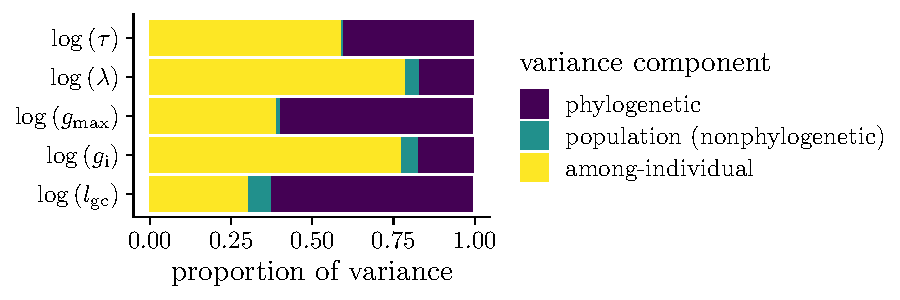
\includegraphics[keepaspectratio]{../figures/variance.pdf}}

}

\caption{\label{fig-variance}\textbf{Traits vary at different levels of biological organization}.
A preponderance of the variation in guard cell length (\gcl)\DIFaddbeginFL \DIFaddFL{, anatomical
maximum stomatal conductance (\gmax), }\DIFaddendFL and the \DIFdelbeginFL \DIFdelFL{time-constant }\DIFdelendFL \DIFaddbeginFL \DIFaddFL{time constant }\DIFaddendFL \(\tau\) is
phylogenetically structured among populations. In contrast, most of the
variance in \DIFaddbeginFL \DIFaddFL{initial }\DIFaddendFL stomatal conductance \DIFdelbeginFL \DIFdelFL{as a fraction
of anatomical maximum stomatal conductance }\DIFdelendFL (\DIFdelbeginFL \DIFdelFL{\fgmax}\DIFdelendFL \DIFaddbeginFL \DIFaddFL{\gi}\DIFaddendFL ) and the \DIFdelbeginFL \DIFdelFL{lag-time
}\DIFdelendFL \DIFaddbeginFL \DIFaddFL{lag time
}\DIFaddendFL (\(\lambda\)) is among individuals. Nonphylogenetic variation among
populations was low for all traits.}

\end{figure}%

\begin{figure}

\centering{

\pandocbounded{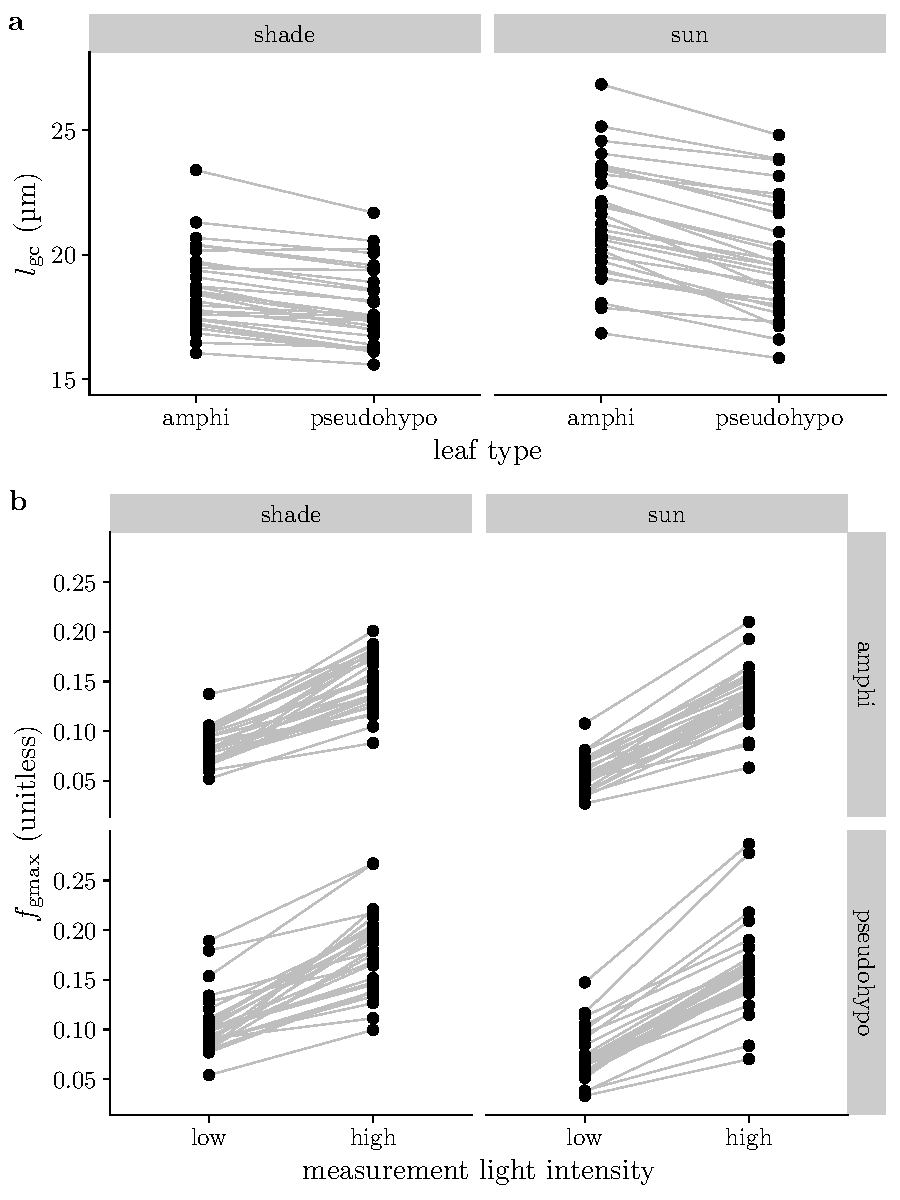
\includegraphics[keepaspectratio]{../figures/accession-anatomy.pdf}}

}

\caption{\label{fig-accession-anatomy}Caption on following page.}

\end{figure}%

\addtocounter{figure}{-1}

\begin{figure}

\centering{

\pandocbounded{
\includegraphics[keepaspectratio]{ms_files/figure-pdf/fig-accession-anatomy-cap-1.pdf}}

}

\caption{\label{fig-accession-anatomy-cap}(previous page)
\textbf{Guard cell length (\gcl) and stomatal conductance as a fraction of maximum conductance (\fgmax) vary among populations and treatments.}
In both panels, black points are mean trait value per population within
a particular treatment. Gray lines connect values within populations
across treatments. (a) Most of the variation in \gcl{} is among
populations, but developmental plasticity to growth light intensity
tends to increase \gcl{} in sun (right facet) compared to shade (left
facet) grown plants. There is no plasticity to leaf type (amphi
vs.~pseudohypo), but the average \gcl{} is slightly lower in pseudohypo
leaves because adaxial stomata tended to be larger than abaxial stomata
on the same leaf. (b) Measurement light intensity has the most direct
effect on \fgmax{} because \DIFaddbeginFL \DIFaddFL{initial }\DIFaddendFL stomatal \DIFdelbeginFL \DIFdelFL{aperture }\DIFdelendFL \DIFaddbeginFL \DIFaddFL{conductance (\gi) }\DIFaddendFL increases
under high light intensity. To a lesser extent, \fgmax{} varies among
populations, is slightly lower in sun-grown plants, and slightly higher
in pseudohypo leaf types.}

\end{figure}%

\subsubsection{Variation in stomatal closure kinetic
parameters}\label{variation-in-stomatal-closure-kinetic-parameters}

Estimates of stomatal closure kinetic parameters for each curve are in
Table~\ref{tbl-estimates-curve} and estimates for each population are in
Table~\ref{tbl-estimates-accession}. \DIFdelbegin \DIFdel{These will be deposited on Dryad
upon publication. The time-constant }\DIFdelend \DIFaddbegin \DIFadd{The time constant }\DIFaddend \(\tau\)
exhibited moderate phylogenetic heritability, accounting for \DIFdelbegin \DIFdel{42.2}\DIFdelend \DIFaddbegin \DIFadd{39.8}\DIFaddend \%
{[}95\% CI: \DIFdelbegin \DIFdel{18.6 to 61.2}\DIFdelend \DIFaddbegin \DIFadd{18.7\% to 60.4}\DIFaddend \%{]} of the variance, whereas \(\lambda\)
varied more within populations
(Figure~\ref{fig-variance}, Table~\ref{tbl-variance}). Some light
treatments also affected kinetic parameters. \DIFdelbegin \DIFdel{In sun plants
,
\(\tau\) was on average 5.56}\DIFdelend \DIFaddbegin \DIFadd{The \(\tau\) in sun plants
was -10.7}\DIFaddend \% {[}95\% CI: \DIFdelbegin \DIFdel{1.05 to 10.4}\DIFdelend \DIFaddbegin \DIFadd{-15.1\% to -6.06}\DIFaddend \%{]} \DIFdelbegin \DIFdel{higher than in }\DIFdelend \DIFaddbegin \DIFadd{lower than }\DIFaddend shade plants
after accounting for other explanatory variables
(Figure~\ref{fig-accession-kinetics}, Table~\ref{tbl-fixed}). Within the
same leaf, increasing the measurement light intensity \DIFdelbegin \DIFdel{prior to the
humidity step change }\DIFdelend from \ppfdqty{150}
to \ppfdqty{2000} significantly increased \(\tau\) by \DIFdelbegin \DIFdel{17.9}\DIFdelend \DIFaddbegin \DIFadd{8.6}\DIFaddend \% {[}95\% CI:
\DIFdelbegin \DIFdel{11.6 to 24.8}\DIFdelend \DIFaddbegin \DIFadd{1.4\% to 16.4}\DIFaddend \%{]}
(Figure~\ref{fig-accession-kinetics}, Table~\ref{tbl-fixed}). The \DIFdelbegin \DIFdel{time
lag
}\DIFdelend \DIFaddbegin \DIFadd{lag
time }\DIFaddend \(\lambda\) responded to growth, but not measurement light
intensity after accounting for other explanatory variables
(Figure~\ref{fig-accession-kinetics}, Table~\ref{tbl-fixed}). In sun
plants, \(\lambda\) was on average \DIFdelbegin \DIFdel{12.2}\DIFdelend \DIFaddbegin \DIFadd{3.43}\DIFaddend \% {[}95\% CI: \DIFdelbegin \DIFdel{10.1 to 14.2}\DIFdelend \DIFaddbegin \DIFadd{1.4\% to 5.67}\DIFaddend \%{]}
greater than in shade plants. High measurement light had little effect
on \(\lambda\), with an estimated \DIFdelbegin \DIFdel{increase of 1.17}\DIFdelend \DIFaddbegin \DIFadd{change of -1.55}\DIFaddend \% {[}95\% CI: \DIFdelbegin \DIFdel{-1.1 to 3.54}\DIFdelend \DIFaddbegin \DIFadd{-4.35\%
to 1.39}\DIFaddend \%{]}.

\begin{figure}

\centering{

\pandocbounded{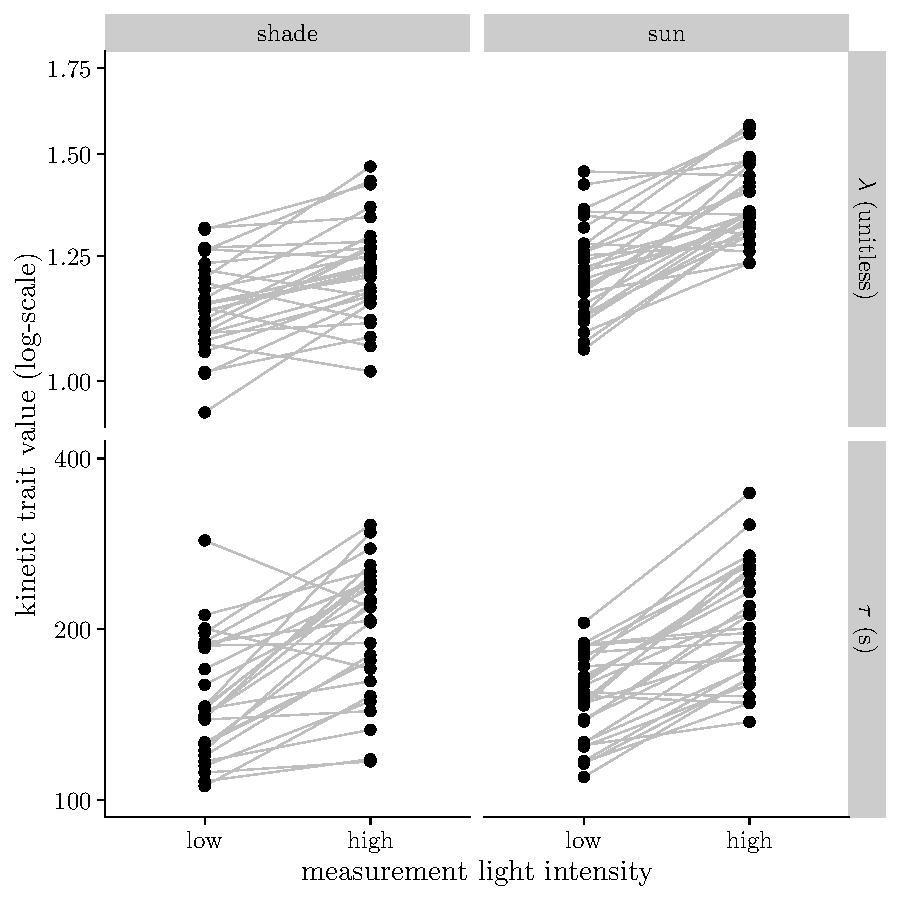
\includegraphics[keepaspectratio]{../figures/accession-kinetics.pdf}}

}

\caption{\label{fig-accession-kinetics}\textbf{Stomatal kinetics parameters $\lambda$ (lag time; top facets) and $\tau$ (time constant; lower facets) vary among wild tomato populations.}
Stomatal conductance decreases faster (lower \(\tau\)) in response to a
step change in vapor pressure deficit (VPD) in leaves when measured
under low light intensity. The pattern was consistent for both shade
(left facets) and sun (right facets) grown plants. The pattern for
\(\lambda\) was qualitatively similar to that for \(\tau\). Each point
is the average parameter value for one accession in that treatment
combination. The growth and measurement light intensity treatments are
described in the Materials and Methods section.}

\end{figure}%

\subsubsection{\DIFdelbegin %DIFDELCMD < \texorpdfstring{Guard cell length and \fgmax{} influence
%DIFDELCMD < stomatal
%DIFDELCMD < kinetics}{Guard cell length and  influence stomatal kinetics}%%%
\DIFdelend \DIFaddbegin \texorpdfstring{Guard cell length and \gi{} influence
stomatal
kinetics}{Guard cell length and  influence stomatal kinetics}\DIFaddend }\label{guard-cell-length-and-influence-stomatal-kinetics}

Guard cell length and \DIFdelbegin \DIFdel{\fgmax{} }\DIFdelend \DIFaddbegin \DIFadd{\gi{}, a component of \fgmax, }\DIFaddend affected stomatal
closure kinetics in the directions predicted by our hypotheses, but they
operated at different levels of biological organization. Among the
models we tested, six were plausible in that their predictive accuracy
was similar based on \(\Delta \mathrm{LOOIC}\)
(Table~\ref{tbl-comparison}). All models in the plausible set indicated
among-individual level effects of \DIFdelbegin \DIFdel{\fgmax{}
}\DIFdelend \DIFaddbegin \DIFadd{\gi{} }\DIFaddend on \(\tau\) and \(\lambda\), as
we discuss in more detail below. Models that included both individual
and phylogenetic effects of \gcl{} had similar LOOIC values but \DIFdelbegin \DIFdel{we selected a model with }\DIFdelend \DIFaddbegin \DIFadd{the
selected model retained }\DIFaddend only phylogenetic effects \DIFdelbegin \DIFdel{for two reasons }\DIFdelend \DIFaddbegin \DIFadd{because our selection
criteria favored models that excluded nonsignificant parameters
}\DIFaddend (Table~\ref{tbl-comparison}). \DIFdelbegin \DIFdel{First, in }\DIFdelend \DIFaddbegin \DIFadd{In }\DIFaddend models that included both individual
and phylogenetic effects, neither the phylogenetic correlation nor the
fixed effect regression coefficient were significantly different \DIFdelbegin \DIFdel{from zero (results not shown}\DIFdelend \DIFaddbegin \DIFadd{than
zero (Figure~\ref{fig-estimates-b}; Figure~\ref{fig-estimates-phy}}\DIFaddend ).
These parameters are highly \DIFdelbegin \DIFdel{colinear }\DIFdelend \DIFaddbegin \DIFadd{collinear }\DIFaddend in the posterior
(Figure~\DIFdelbegin \DIFdel{\ref{fig-colinear}}\DIFdelend \DIFaddbegin \DIFadd{\ref{fig-collinear}}\DIFaddend ) indicating difficulty in estimating both
terms simultaneously and ``smearing'' out their confidence intervals
(McElreath, 2020). Hence, the model with only phylogenetic effects is
easier to interpret. \DIFdelbegin \DIFdel{The second reason we favor this model is that it is
}\DIFdelend \DIFaddbegin \DIFadd{This model is also }\DIFaddend consistent with the high
phylogenetic heritability in both \gcl{} and \(\tau\)
(Figure~\ref{fig-variance}). Visually, we observed positive
relationships among population mean trait values
(Figure~\ref{fig-gcl-tau}) but little relationship between \gcl{} and
\(\tau\) within populations (results not shown). When comparing many
models simultaneously, differences in LOOIC performance can occur by
chance (McLatchie \& Vehtari, 2024), so judgement calls among models
with similar performance can be necessary. The preponderance of evidence
indicates that \gcl{} explains variation primarily among rather than
within our populations. The results in the main text are based on
estimates from the selected model. \DIFaddbegin \DIFadd{Individual-level fixed effects
(Figure~\ref{fig-estimates-b}) and phylogenetic correlations
(Figure~\ref{fig-estimates-phy}) of \gcl, \gi, and \gmax{} on \(\tau\)
and \(\lambda\) were qualitatively consistent across all plausible
models.
}\DIFaddend 

\DIFdelbegin %DIFDELCMD < \begin{table}
%DIFDELCMD < 

%DIFDELCMD < %%%
%DIFDELCMD < \caption{%
{%DIFAUXCMD
%DIFDELCMD < \label{tbl-comparison}%%%
\DIFdelFL{Model comparison results. Models with a
\(\Delta\)LOOIC less than two standard errors (SE) from the minimum
LOOIC are considered to have substantial support and are used for
posterior predictions to test hypotheses about the effects of guard cell
length (\gcl) and the stomatal conductance as a fraction of anatomical
maximum stomatal conductance (\fgmax) on stomatal kinetic parameter
\(\lambda\) (time lag) and \(\tau\) (time constant). Unsupported models
are in gray italic font. The model selected for subsequent inference is
in bold. LOOIC stands for leave-one-out cross-validation information
criterion.}}
%DIFAUXCMD
%DIFDELCMD < 

%DIFDELCMD < \centering{
%DIFDELCMD < 

%DIFDELCMD < \begin{tabular}[t]{llcccc}
%DIFDELCMD < \toprule
%DIFDELCMD < \multicolumn{2}{c}{ } & \multicolumn{2}{c}{$\lambda$} & \multicolumn{2}{c}{$\tau$} \\
%DIFDELCMD < \cmidrule(l{3pt}r{3pt}){3-4} \cmidrule(l{3pt}r{3pt}){5-6}
%DIFDELCMD < $\Delta \mathrm{LOOIC}$ & SE & \fgmax & \gcl & \fgmax & \gcl\\
%DIFDELCMD < \midrule
%DIFDELCMD < 0.00 & 0.00 & \cmark & \cmark & \cmark & \cmark\\
%DIFDELCMD < \textbf{1.38} & \textbf{3.08} & \textbf{\cmark} & \textbf{} & \textbf{\cmark} & \textbf{}\\
%DIFDELCMD < 1.91 & 3.14 & \cmark & \cmark & \cmark & \\
%DIFDELCMD < 2.83 & 3.04 & \cmark &  & \cmark & \cmark\\
%DIFDELCMD < 16.16 & 10.83 & \cmark & \cmark &  & \\
%DIFDELCMD < \addlinespace
%DIFDELCMD < 17.77 & 10.84 & \cmark &  &  & \\
%DIFDELCMD < \textcolor{gray}{\em{23.79}} & \textcolor{gray}{\em{10.76}} & \textcolor{gray}{\em{\cmark}} & \textcolor{gray}{\em{\cmark}} & \textcolor{gray}{\em{}} & \textcolor{gray}{\em{\cmark}}\\
%DIFDELCMD < \textcolor{gray}{\em{24.29}} & \textcolor{gray}{\em{10.94}} & \textcolor{gray}{\em{\cmark}} & \textcolor{gray}{\em{}} & \textcolor{gray}{\em{}} & \textcolor{gray}{\em{\cmark}}\\
%DIFDELCMD < \textcolor{gray}{\em{46.64}} & \textcolor{gray}{\em{14.58}} & \textcolor{gray}{\em{}} & \textcolor{gray}{\em{\cmark}} & \textcolor{gray}{\em{\cmark}} & \textcolor{gray}{\em{}}\\
%DIFDELCMD < \textcolor{gray}{\em{47.79}} & \textcolor{gray}{\em{14.48}} & \textcolor{gray}{\em{}} & \textcolor{gray}{\em{\cmark}} & \textcolor{gray}{\em{\cmark}} & \textcolor{gray}{\em{\cmark}}\\
%DIFDELCMD < \addlinespace
%DIFDELCMD < \textcolor{gray}{\em{49.54}} & \textcolor{gray}{\em{14.63}} & \textcolor{gray}{\em{}} & \textcolor{gray}{\em{}} & \textcolor{gray}{\em{\cmark}} & \textcolor{gray}{\em{}}\\
%DIFDELCMD < \textcolor{gray}{\em{50.34}} & \textcolor{gray}{\em{14.54}} & \textcolor{gray}{\em{}} & \textcolor{gray}{\em{}} & \textcolor{gray}{\em{\cmark}} & \textcolor{gray}{\em{\cmark}}\\
%DIFDELCMD < \textcolor{gray}{\em{68.81}} & \textcolor{gray}{\em{18.41}} & \textcolor{gray}{\em{}} & \textcolor{gray}{\em{\cmark}} & \textcolor{gray}{\em{}} & \textcolor{gray}{\em{}}\\
%DIFDELCMD < \textcolor{gray}{\em{71.66}} & \textcolor{gray}{\em{18.38}} & \textcolor{gray}{\em{}} & \textcolor{gray}{\em{}} & \textcolor{gray}{\em{}} & \textcolor{gray}{\em{\cmark}}\\
%DIFDELCMD < \textcolor{gray}{\em{72.76}} & \textcolor{gray}{\em{18.48}} & \textcolor{gray}{\em{}} & \textcolor{gray}{\em{}} & \textcolor{gray}{\em{}} & \textcolor{gray}{\em{}}\\
%DIFDELCMD < \addlinespace
%DIFDELCMD < \textcolor{gray}{\em{75.18}} & \textcolor{gray}{\em{18.39}} & \textcolor{gray}{\em{}} & \textcolor{gray}{\em{\cmark}} & \textcolor{gray}{\em{}} & \textcolor{gray}{\em{\cmark}}\\
%DIFDELCMD < \bottomrule
%DIFDELCMD < \end{tabular}
%DIFDELCMD < 

%DIFDELCMD < }
%DIFDELCMD < 

%DIFDELCMD < \end{table}%%%
%DIF < 
%DIFDELCMD < 

%DIFDELCMD < %%%
\DIFdel{Leaves with stomatal apertures closer to their maximum aperture }\DIFdelend \DIFaddbegin \DIFadd{Leaves with greater \gi{} }\DIFaddend closed more slowly than those \DIFaddbegin \DIFadd{which were }\DIFaddend less
open (Figure~\DIFdelbegin \DIFdel{\ref{fig-fgmax-tau}}\DIFdelend \DIFaddbegin \DIFadd{\ref{fig-gi-tau}; Table~\ref{tbl-fixed}}\DIFaddend ). For example,
increasing \DIFdelbegin \DIFdel{\fgmax{} from 20\% to
30\% }\DIFdelend \DIFaddbegin \DIFadd{\gi{} from 0.2 to
\(\SI{0.4}{\mole\per\meter\squared\per\second}\) }\DIFaddend resulted in a \DIFdelbegin \DIFdel{10.7}\DIFdelend \DIFaddbegin \DIFadd{25.1}\DIFaddend \%
{[}95\% CI: \DIFdelbegin \DIFdel{7.2 to 14.4}\DIFdelend \DIFaddbegin \DIFadd{17.6\% to 32.6}\DIFaddend \%{]} increase in \(\tau\) for a typical leaf
in the reference treatment set (shade, low, amphi). \DIFdelbegin \DIFdel{The \fgmax{} }\DIFdelend \DIFaddbegin \DIFadd{We found little
evidence that \gmax{} affected \(\tau\) (Figure~\ref{fig-gmax-tau}).
Leaves with greater \gi{} }\DIFaddend also had a \DIFdelbegin \DIFdel{significant,
positive, individual-level effect on \(\lambda\)
(Table~\ref{tbl-fixed}}\DIFdelend \DIFaddbegin \DIFadd{significantly greater lag time,
\(\lambda\) (Figure~\ref{fig-gi-lambda}), but there was little effect of
\gmax{} (Figure~\ref{fig-gmax-lambda}}\DIFaddend ).

Populations that tended to have greater \gcl{} also tended to have
greater \(\tau\) as evidenced by a positive phylogenetic correlation
(Table~\ref{tbl-random}, Figure~\ref{fig-gcl-tau}). However, we found
little evidence that variation in \gcl{} explained \(\tau\) or
\(\lambda\) within populations. There were no other significant
phylogenetic correlations (Table~\ref{tbl-random}). The only marginally
significant partial correlation was between \gcl{} and \(\tau\)
(\DIFdelbegin \DIFdel{\(\rho = 0.74\) }\DIFdelend \DIFaddbegin \DIFadd{\(\rho = 0.71\) }\DIFaddend {[}95\% CI: \DIFdelbegin \DIFdel{\(-0.18\) }\DIFdelend \DIFaddbegin \DIFadd{\(-0.17\) }\DIFaddend to \(0.98\){]}), indicating a
plausible causal effect of \gcl{} on \(\tau\) among populations.

\begin{figure}

\centering{

\pandocbounded{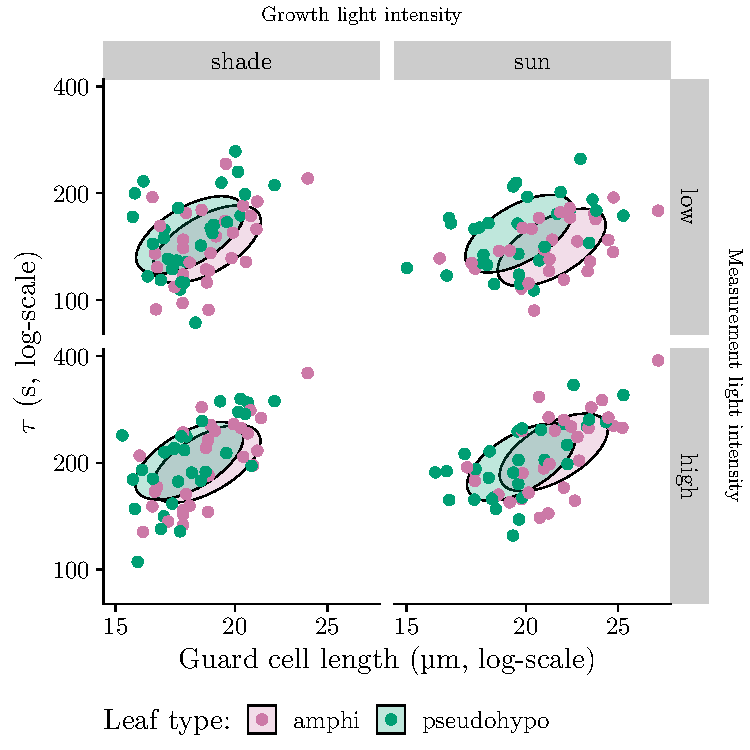
\includegraphics[keepaspectratio]{../figures/gcl-tau.pdf}}

}

\caption{\label{fig-gcl-tau}\DIFdelbeginFL \textbf{\DIFdelFL{Phylogenetic covariance between guard cell length (\gcl, $x$-axis) and the stomatal closure time-constant ($\tau$, $y$-axis) indicates that populations with larger stomata tend to close more slowly in response to humidity.}}
%DIFAUXCMD
\DIFdelendFL \DIFaddbeginFL \textbf{\DIFaddFL{Phylogenetic covariance between guard cell length (\gcl, $x$-axis) and the stomatal closure time constant ($\tau$, $y$-axis) indicates that populations with larger stomata tend to close more slowly in response to humidity.}}
\DIFaddendFL The overall pattern was consistent across growth light intensity
treatments (left and right facets), measurement light intensity
treatments (top and bottom facets), and leaf types (point colors). The
direction and magnitude of the ellipses are such that they should
encompass 95\% of the phylogenetically structured (co)variance in \gcl{}
and \(\tau\) on log-transformed scales. The location of ellipses are set
to the median trait values in each treatment combination for visual
comparison. Each point is the average parameter value for one \DIFdelbeginFL \DIFdelFL{accession
}\DIFdelendFL \DIFaddbeginFL \DIFaddFL{population
}\DIFaddendFL in that treatment combination. The growth and measurement light
intensity treatments are described in the Materials and Methods
section.}

\end{figure}%

\begin{figure}

\DIFdelbeginFL %DIFDELCMD < \centering{
%DIFDELCMD < 

%DIFDELCMD < \pandocbounded{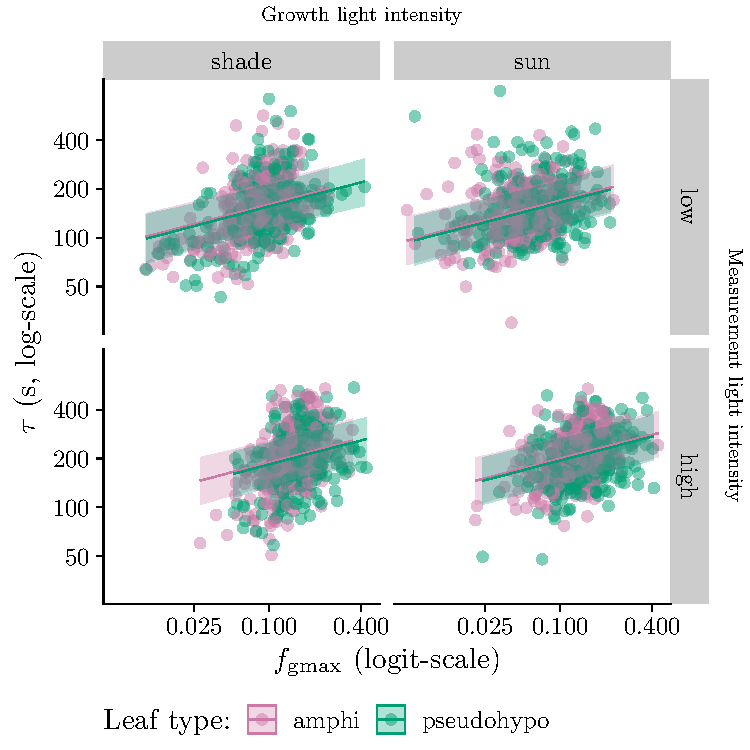
\includegraphics[keepaspectratio]{../figures/fgmax-tau.pdf}}
%DIFDELCMD < 

%DIFDELCMD < }
%DIFDELCMD < %%%
\DIFdelendFL \DIFaddbeginFL \centering{

\pandocbounded{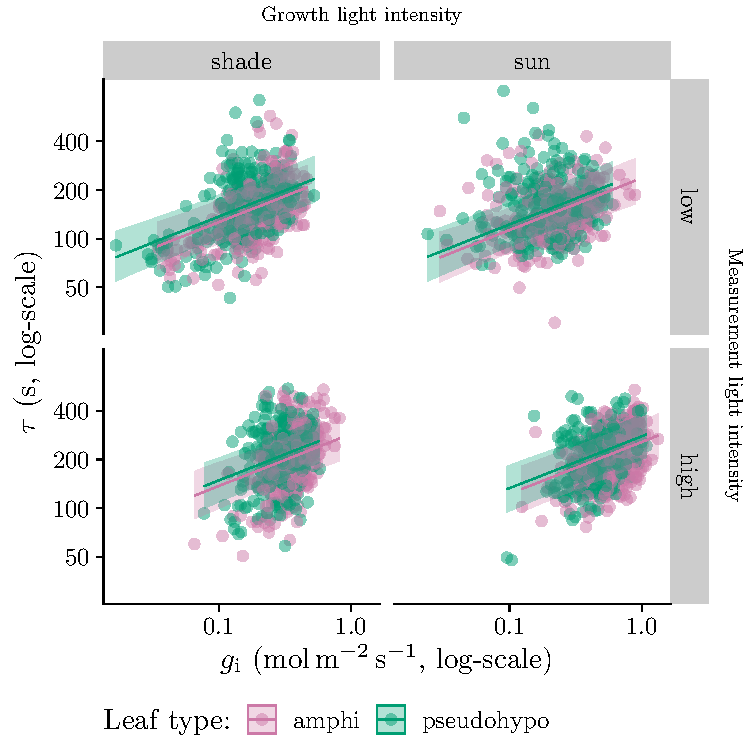
\includegraphics[keepaspectratio]{../figures/gi-tau.pdf}}

}
\DIFaddendFL 

\caption{\DIFdelbeginFL %DIFDELCMD < \label{fig-fgmax-tau}%%%
\textbf{\DIFdelFL{Individual-level variation in stomatal apertures influences stomatal closures kinetics.}}
%DIFAUXCMD
\DIFdelendFL \DIFaddbeginFL \label{fig-gi-tau}\textbf{\DIFaddFL{Individual-level variation in initial stomatal conductance (\gi) influences stomatal closure kinetics.}}
\DIFaddendFL As \DIFdelbeginFL \DIFdelFL{the stomatal conductance as a fraction of anatomical maximum stomatal
conductance }\DIFdelendFL \DIFaddbeginFL \DIFaddFL{\gi{} }\DIFaddendFL (\DIFdelbeginFL \DIFdelFL{\fgmax, }\DIFdelendFL \(x\)-axis) \DIFdelbeginFL \DIFdelFL{increase}\DIFdelendFL \DIFaddbeginFL \DIFaddFL{increases}\DIFaddendFL , the stomatal closure \DIFdelbeginFL \DIFdelFL{time-constant }\DIFdelendFL \DIFaddbeginFL \DIFaddFL{time constant
}\DIFaddendFL (\(\tau\), \(y\)-axis) increases. The overall pattern was consistent
across grow light intensity treatments (left and right facets),
measurement light intensity treatments (top and bottom facets), and leaf
types (point colors). Lines are estimated using linear regression along
with 95\% confidence ribbons. The growth and measurement light intensity
treatments are described in the Materials and Methods section.}

\end{figure}%

\subsubsection{\DIFdelbegin %DIFDELCMD < \texorpdfstring{Stomatal aperture mediates plasticity in
%DIFDELCMD < \(\tau\)}{Stomatal aperture mediates plasticity in \textbackslash tau}%%%
\DIFdelend \DIFaddbegin \texorpdfstring{Plasticity in \(\tau\) is an indirect
effect of plasticity in
\gi}{Plasticity in \textbackslash tau is an indirect effect of plasticity in }\DIFaddend }\DIFdelbegin %DIFDELCMD < \label{stomatal-aperture-mediates-plasticity-in-tau}
%DIFDELCMD < %%%
\DIFdelend \DIFaddbegin \label{plasticity-in-tau-is-an-indirect-effect-of-plasticity-in}
\DIFaddend 

We imposed three treatments that influenced stomatal kinetics: growth
light intensity, measurement light intensity, and leaf type. All three
treatments directly affected \(\tau\) and had indirect effects mediated
by \DIFdelbegin \DIFdel{\fgmax{} }\DIFdelend \DIFaddbegin \DIFadd{\gi{} }\DIFaddend (Figure~\ref{fig-mediation}). We did not estimate effects
mediated by \gcl{} because the selected model did not retain direct
effects of \gcl{} on \(\tau\) (Table~\ref{tbl-comparison}). The \DIFdelbegin \DIFdel{direct
effect of the sun growth treatment }\DIFdelend \DIFaddbegin \DIFadd{indirect
effect of greater \gi{} in sun leaves }\DIFaddend increased \(\tau\) by \DIFdelbegin \DIFdel{\(5.58\)}\DIFdelend \DIFaddbegin \DIFadd{\(11.78\)}\DIFaddend \%
{[}95\% CI: \DIFdelbegin \DIFdel{\(1.05\) to \(10.44\)}\DIFdelend \DIFaddbegin \DIFadd{\(8.27\)\% to \(15.99\)}\DIFaddend \%{]}, \DIFdelbegin \DIFdel{but the indirect effectof lower
\fgmax{} counteracted it by \(-5.06\)\% }%DIFDELCMD < {[}%%%
\DIFdel{95\% CI: \(-7.30\) to
\(-3.18\)\%}%DIFDELCMD < {]}%%%
\DIFdelend \DIFaddbegin \DIFadd{counteracting the direct
negative effect}\DIFaddend . The direct effect of the pseudohypo treatment \DIFdelbegin \DIFdel{decreased
}\DIFdelend \DIFaddbegin \DIFadd{increased
}\DIFaddend \(\tau\) \DIFdelbegin \DIFdel{slightly by \(-2.64\)}\DIFdelend \DIFaddbegin \DIFadd{by \(8.60\)}\DIFaddend \% {[}95\% CI: \DIFdelbegin \DIFdel{\(-4.98\) to \(-0.15\)}\DIFdelend \DIFaddbegin \DIFadd{\(5.62\)\% to \(11.56\)}\DIFaddend \%{]}, but the
indirect effect mediated by \DIFdelbegin \DIFdel{greater \fgmax{}
increased }\DIFdelend \DIFaddbegin \DIFadd{lower \gi{} changed }\DIFaddend \(\tau\) by \DIFdelbegin \DIFdel{\(4.02\)}\DIFdelend \DIFaddbegin \DIFadd{\(-6.72\)}\DIFaddend \%
{[}95\% CI: \DIFdelbegin \DIFdel{\(2.64\) to \(5.49\)}\DIFdelend \DIFaddbegin \DIFadd{\(-8.64\)\% to \(-4.83\)}\DIFaddend \%{]}. In contrast, direct and
indirect effects of high measurement light intensity increased \(\tau\).
The direct effect increased \(\tau\) by \DIFdelbegin \DIFdel{\(17.90\)}\DIFdelend \DIFaddbegin \DIFadd{\(8.56\)}\DIFaddend \% {[}95\% CI:
\DIFdelbegin \DIFdel{\(11.63\) to \(24.82\)}\DIFdelend \DIFaddbegin \DIFadd{\(1.40\)\% to \(16.40\)}\DIFaddend \%{]} and the indirect effect mediated by \DIFdelbegin \DIFdel{\fgmax{} }\DIFdelend \DIFaddbegin \DIFadd{\gi{}
}\DIFaddend increased \(\tau\) by \DIFdelbegin \DIFdel{\(17.31\)}\DIFdelend \DIFaddbegin \DIFadd{\(27.62\)}\DIFaddend \% {[}95\% CI: \DIFdelbegin \DIFdel{\(11.34\) to
\(23.48\)}\DIFdelend \DIFaddbegin \DIFadd{\(19.18\)\% to
\(36.24\)}\DIFaddend \%{]}.

\begin{figure}

\centering{

\pandocbounded{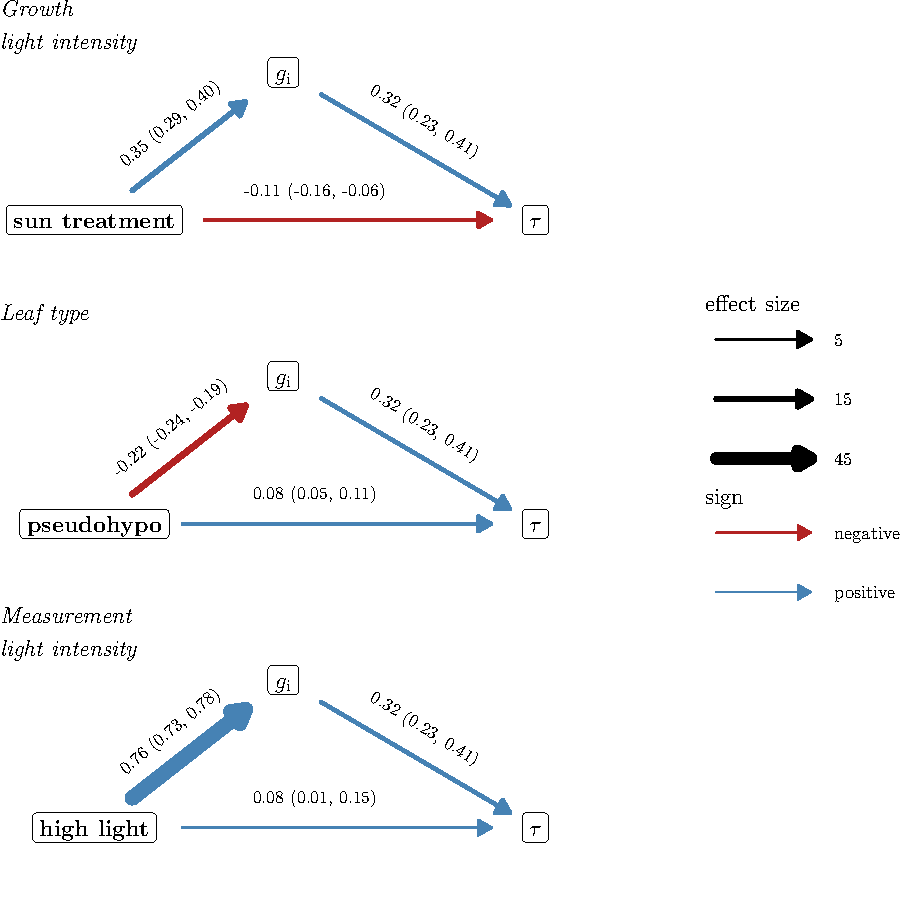
\includegraphics[keepaspectratio]{../figures/mediation.pdf}}

}

\caption{\label{fig-mediation}\DIFdelbeginFL \textbf{\DIFdelFL{Stomatal aperture as a fraction of anatomical maximum stomatal conductance (\fgmax) mediates plasticity in the time constant $\tau$.}}
%DIFAUXCMD
\DIFdelendFL \DIFaddbeginFL \textbf{\DIFaddFL{Treatment-associated plasticity in the time constant $\tau$ is statistically consistent with an indirect path through initial stomatal conductance (\gi).}}
\DIFaddendFL The three treatments are growth light intensity (top facet; shade
vs.~sun), leaf type (middle facet; amphi vs.~pseudohypo), and
measurement light intensity (bottom facet; low vs.~high). Horizontal
arrows at the bottom of each graph indicate the direct effect of the
treatment level on \(\tau\); slanted arrows leading to or from \DIFdelbeginFL \DIFdelFL{\fgmax{}
}\DIFdelendFL \DIFaddbeginFL \DIFaddFL{\gi{}
}\DIFaddendFL indicate \DIFdelbeginFL \DIFdelFL{mediated }\DIFdelendFL \DIFaddbeginFL \DIFaddFL{indirect }\DIFaddendFL effects of the treatment on \(\tau\) \DIFaddbeginFL \DIFaddFL{through \gi{}}\DIFaddendFL .
Line thickness is proportional to the effect size and line color
indicates whether the effects are negative (red) \DIFaddbeginFL \DIFaddFL{or }\DIFaddendFL positive (blue).
Parameter estimates of the effect and 95\% confidence intervals are
above each line. The selected model did not retain direct effects of
\gcl{} on \(\tau\) and hence this variable could not be \DIFdelbeginFL \DIFdelFL{considered as }\DIFdelendFL \DIFaddbeginFL \DIFaddFL{included in this
analysis. This path analysis assumes sequential ignorability (no
unmeasured confounder of the \gi{}-\(\tau\) relationship); see Notes S3
for }\DIFaddendFL a \DIFdelbeginFL \DIFdelFL{mediator}\DIFdelendFL \DIFaddbeginFL \DIFaddFL{sensitivity analysis of this assumption}\DIFaddendFL .}

\end{figure}%

\subsubsection{\DIFdelbegin \DIFdel{No evidence that adaxial stomata close faster than
abaxial
stomata}\DIFdelend \DIFaddbegin \texorpdfstring{Adaxial stomata close faster than abaxial
stomata, but the effect is masked by plasticity in
\gi{}}{Adaxial stomata close faster than abaxial stomata, but the effect is masked by plasticity in }\DIFaddend }\DIFdelbegin %DIFDELCMD < \label{no-evidence-that-adaxial-stomata-close-faster-than-abaxial-stomata}
%DIFDELCMD < %%%
\DIFdelend \DIFaddbegin \label{adaxial-stomata-close-faster-than-abaxial-stomata-but-the-effect-is-masked-by-plasticity-in}
\DIFaddend 

\DIFdelbegin \DIFdel{The time constant }\DIFdelend \DIFaddbegin \DIFadd{Although a simple comparison of }\DIFaddend \(\tau\) \DIFdelbegin \DIFdel{was slightly greater in pseudohypo leaves
compared to the paired amphi leaf }\DIFdelend \DIFaddbegin \DIFadd{between paired amphi and
pseudohypo leaf types shows little net difference }\DIFaddend (results not shown),
\DIFdelbegin \DIFdel{which would
suggest }\DIFdelend \DIFaddbegin \DIFadd{the selected model reveals a significant direct effect of leaf type on
\(\tau\) once \gi{} is accounted for: pseudohypo leaves, which have only
abaxial stomata, closed more slowly than amphi leaves
(Figure~\ref{fig-mediation}; Table~\ref{tbl-fixed}). This direct effect
is consistent with the hypothesis }\DIFaddend that adaxial stomata close faster \DIFaddbegin \DIFadd{than
abaxial stomata}\DIFaddend . However, pseudohypo leaves also had \DIFdelbegin \DIFdel{greater \fgmax, which slows stomatal closure
, as discussed in
the previous section. Once, the indirect effect of \fgmax{} on \(\tau\)
is accounted for, }\DIFdelend \DIFaddbegin \DIFadd{lower \gi{} and
lower \gi{} is itself associated with faster closure
(Figure~\ref{fig-gi-tau}). This indirect path through \gi{} counteracts
most of }\DIFaddend the direct effect \DIFdelbegin \DIFdel{of pseudohypo leaf type on \(\tau\)
disappears, indicating that the observed difference in \(\tau\) between
pseudohypo and amphi leaves is mediated by \fgmax{}
}\DIFdelend (Figure~\ref{fig-mediation})\DIFdelbegin \DIFdel{. There is actually a tendency for \(\tau\)
to be slightly lower when only abaxial stomata are measured in
pseudohypo leaves, as evidenced by the
negative effect of this leaf type
on \(\tau\) (Table~\ref{tbl-fixed})}\DIFdelend \DIFaddbegin \DIFadd{, which is why the
raw comparison of paired leaves does not reveal much difference in
kinetics between leaf types even though adaxial stomata appear to close
faster once \gi{} is controlled for}\DIFaddend .

\subsection{Discussion}\label{discussion}

The ability for stomata to adjust to fluctuating environmental
conditions likely evolved in early land plants because of selection to
optimize water use relative to carbon gain (Raven, 2002). Hydroactive
control of stomatal aperture in angiosperms increases flexibility to
modulate carbon gain and water loss depending on leaf water status
(Buckley, 2019), perhaps enabling a competitive advantage in
environments where light and evaporative demand fluctuate at high
frequency (McAdam \& Brodribb, 2012, 2015\DIFaddbegin \DIFadd{; Pichaco }\emph{\DIFadd{et al.}}\DIFadd{, 2026}\DIFaddend ).
We now understand the steady-state response of stomatal conductance
(\gsw) to global increases in vapor pressure deficit (VPD) better but
there is greater uncertainty surrounding kinetic responses to VPD
(Buckley \emph{et al.}, 2023). Here we considered two nonmutually
exclusive mechanistic hypotheses for how stomatal anatomy influences
stomatal closure kinetics. First, smaller stomata may close faster
because of greater surface area to volume ratio (Drake \emph{et al.},
2013). Second, guard cells under higher turgor pressure respond more
slowly because of reduced cell wall elasticity (Franks \emph{et al.},
2012). Based on these hypotheses, we predicted that leaves with smaller
guard cells and operating further from their anatomical maximum \gsw{}
(i.e., lower \fgmax) would have faster stomatal closure kinetics (lower
\(\tau\)). \DIFaddbegin \DIFadd{The parameter \fgmax{} is here defined as the initial
stomatal conductance (\gi) divided by \gmax. }\DIFaddend Analysis of 2,\DIFdelbegin \DIFdel{124 }\DIFdelend \DIFaddbegin \DIFadd{125 }\DIFaddend time
courses of stomatal closure from 29 populations in multiple environments
demonstrates that both guard cell size and \DIFdelbegin \DIFdel{stomatal aperture }\DIFdelend \DIFaddbegin \DIFadd{\gi{}, a component of \fgmax,
}\DIFaddend influence kinetics at different levels of biological organization. This
new understanding suggests unexplored explanations for the relationships
between stomatal size, density, speed, and operational \gsw{} (\gop)
among \DIFdelbegin \DIFdel{land plants}\DIFdelend \DIFaddbegin \DIFadd{angiosperms}\DIFaddend .

The kinetics of stomatal closure in response to VPD closely match
response to light, suggesting similar underlying mechanisms. The
lag-time model proposed by Woning \emph{et al.} (2026) for light
responses also describes humidity responses extremely well following the
passive wrong-way response \DIFaddbegin \DIFadd{(WWR)}\DIFaddend . The fitted models explained on average
99.94\% of the variation in \gsw{} during closure
(Figure~\ref{fig-rh-curves}). The formal mathematical similarity of
light and humidity response might indicate that certain factors, \DIFdelbegin \DIFdel{like
}\DIFdelend \DIFaddbegin \DIFadd{such as
}\DIFaddend guard cell size, influence stomatal kinetics responses in general.
Alternatively, disparate underlying processes may be described by the
same macroscale formalism. For example, humidity responses may be
controlled by ABA accumulation or loss (McAdam \emph{et al.}, 2016),
whereas \(C_\mathrm{i}\)-independent red-light responses can be
influenced by accumulation or loss of photosynthetic products (Matthews
\emph{et al.}, 2020). These disparate processes may both have similar
kinetic properties, but would not necessarily imply that VPD and light
responses are strongly correlated. Future research comparing the
correlation between light, VPD, CO\textsubscript{2}, and other stomatal
kinetic responses can determine the extent to which generic or specific
factors determine stomatal opening and closing rates (Creese \emph{et
al.}, 2014; Kübarsepp \emph{et al.}, 2020).

The positive association between \gcl{} and \(\tau\)
(Figure~\ref{fig-gcl-tau}) is consistent with the hypothesis that
smaller cells respond faster because they have a greater surface area to
volume ratio for osmolyte flux (Franks \& Farquhar, 2007; Drake \emph{et
al.}, 2013; Lawson \& Vialet-Chabrand, 2019; Woning \emph{et al.},
2026). \DIFdelbegin \DIFdel{If correct, this }\DIFdelend \DIFaddbegin \DIFadd{Among several of the same }\emph{\DIFadd{Solanum}} \DIFadd{species, larger guard
cells are also associated with slower opening kinetics in response to
light (Yoshiyama }\emph{\DIFadd{et al.}}\DIFadd{, 2024), suggesting a general mechanism.
Specifically, this association }\DIFaddend implies that the maximum rate of stomatal
closure is limited by membrane surface area. We do not have the data to
evaluate the hypothesis mechanistically, but this should be tested in
the future. \DIFaddbegin \DIFadd{In addition to guard cell size, it will be useful to test
whether the ratio of guard cell to adjacent epidermal size affects the
strength of the WWR, which may be necessary to induce more rapid
stomatal closure (Buckley }\emph{\DIFadd{et al.}}\DIFadd{, 2003; Pichaco }\emph{\DIFadd{et al.}}\DIFadd{,
2025). }\DIFaddend An alternative explanation is that the correlation between \gcl{}
and \(\tau\) is not causal. The fact that \gcl{} did not explain much of
the variation in \(\tau\) among individuals within populations suggests
that \gcl{} may not directly affect \(\tau\). However, the high
phylogenetic heritability and, hence, low variability in \gcl{} within
populations may also explain why we were unable to detect a
within-population effect of \gcl{} on \(\tau\).

A \DIFaddbegin \DIFadd{potential }\DIFaddend consequence of greater stomatal aperture is that \DIFdelbegin \DIFdel{they close }\DIFdelend \DIFaddbegin \DIFadd{the pore
closes }\DIFaddend more slowly when the environment changes. Much of the variation
in \(\tau\) among individuals within populations was explained by
variation in \DIFdelbegin \DIFdel{\fgmax{} }\DIFdelend \DIFaddbegin \DIFadd{\gi{} }\DIFaddend (Figure~\DIFdelbegin \DIFdel{\ref{fig-fgmax-tau}}\DIFdelend \DIFaddbegin \DIFadd{\ref{fig-gi-tau}}\DIFaddend ). This \DIFaddbegin \DIFadd{association is not
simply an artifact of the magnitude of the difference between \gi{} and
\gf{}, because \(\tau\) captures the proportional rate of change, not
the absolute change, in \gsw. This }\DIFaddend factor was positively associated with
\(\tau\) among individuals \DIFdelbegin \DIFdel{in the same combination of
}\DIFdelend \DIFaddbegin \DIFadd{within }\DIFaddend light treatments, \DIFdelbegin \DIFdel{but also mediated much of the plastic effects of these
treatments on }\DIFdelend \DIFaddbegin \DIFadd{and
treatment-associated plasticity in }\DIFaddend \(\tau\) \DIFaddbegin \DIFadd{was statistically consistent
with an indirect path through \gi{} }\DIFaddend (Figure~\ref{fig-mediation}). \DIFdelbegin \DIFdel{To our knowledge,
this relationship has not been previously documented. However, the }\DIFdelend \DIFaddbegin \DIFadd{The
}\DIFaddend rate of stomatal opening in response to light is associated with \gop{}
in a sample of rainforest trees (Kardiman \& Ræbild, 2018), which may
indicate this is a more general phenomenon.
\DIFaddbegin 

\DIFaddend The association between \DIFdelbegin \DIFdel{\fgmax{} }\DIFdelend \DIFaddbegin \DIFadd{\gi{} }\DIFaddend and \(\tau\) could be explained by the
hypothesis that guard cell wall elasticity declines at greater turgor
pressure (Franks \emph{et al.}, 2012), like a rubber band that is
stretched under tension. \DIFaddbegin \DIFadd{However, if this were the case, we would also
expect a negative association between \gmax{} and \(\tau\) because
leaves with greater \gmax{} could have the same \gi{} with a smaller
stomatal aperture. However, this effect was weakly supported
(Figure~\ref{fig-gmax-tau}, Figure~\ref{fig-gmax-lambda}). The selected
model did not include an individual-level effect of \gmax{} on kinetic
parameters. Although the second-best model included \gmax{} and the
effect was in the predicted direction (Table~\ref{tbl-comparison}), the
effect was not significantly different than 0
(Figure~\ref{fig-estimates-b}). The weak effect of \gmax{} compared to
\gi{} casts doubt on whether a nonlinear relationship between turgor
pressure and pore aperture is the best explanation. An alternative,
albeit not mutually exclusive explanation, is a nonlinear relationship
between pore aperture and \gsw{} that weakens the association between
these variables at high \gsw. Airspace resistance within the substomatal
cavity and stomatal interference are plausible mechanisms that would
have this effect (Ting \& Loomis, 1965; Kaiser, 2009; Lehmann \& Or,
2015), although it is not clear that they are sufficient to produce the
observed relationship between \gi{} and \(\tau\) in wild tomatoes. Our
study is limited by the fact that we did not directly measure guard cell
turgor or stomatal aperture, but future studies should use newly
developed methods (Brodersen }\emph{\DIFadd{et al.}}\DIFadd{, 2025) to directly evaluate
the association between these traits.
}\DIFaddend 

The impact of \DIFdelbegin \DIFdel{\fgmax{} }\DIFdelend \DIFaddbegin \DIFadd{\gi{} }\DIFaddend was most pronounced when comparing measurement light
intensity treatments. Leaves acclimated to high light intensity were on
average \DIFdelbegin \DIFdel{111}\DIFdelend \DIFaddbegin \DIFadd{113}\DIFaddend \% more open than the same leaves at low light intensity in
the reference treatment (shade, amphi). As a consequence, stomata closed
more slowly in leaves acclimated to high light intensity, with a \DIFdelbegin \DIFdel{17.3\%
greater time-constant }\DIFdelend \DIFaddbegin \DIFadd{27.6\%
greater time constant }\DIFaddend on average in the reference treatment, based on
parameter estimates from the selected model (Table~\ref{tbl-fixed}). We
did not assess whether \DIFdelbegin \DIFdel{\fgmax{} }\DIFdelend \DIFaddbegin \DIFadd{\gi{} }\DIFaddend also affects stomatal opening and this
should be measured to further test this hypothesis. The implication is
that natural selection should favor \gop{} values that not only optimize
instantaneous carbon gain and water loss in the present environment, but
also carbon gain and water loss integrated through time in a fluctuating
environment. We predict that rapid, temporally-uncorrelated fluctuating
environments will favor leaves with greater \DIFdelbegin \DIFdel{\fgmax{} }\DIFdelend \DIFaddbegin \DIFadd{\gop{} }\DIFaddend to slow kinetic
responses and prevent overreacting to transitory changes that are likely
to revert; slower, temporally-correlated changes will favor lower \DIFdelbegin \DIFdel{\fgmax{} }\DIFdelend \DIFaddbegin \DIFadd{\gop{}
}\DIFaddend to enable close tracking of the environment.

The \DIFdelbegin \DIFdel{absence of a }\DIFdelend \DIFaddbegin \DIFadd{comparison between measurement light intensity treatments should be
interpreted cautiously, however, because it was confounded with
measurement order: high light curves always preceded low light curves on
the same leaf, following a prior low-humidity closure event (see
Materials and Methods). We cannot rule out that some of the apparent
effect of measurement light intensity on \gi{} and \(\tau\), and the
corresponding indirect path through \gi{} in our mediation analysis
(Figure~\ref{fig-mediation}), reflects order, incomplete recovery, or
prior VPD exposure rather than measurement light intensity itself. This
concern applies specifically to the measurement light comparison and not
to growth light intensity or leaf type, which were randomized or
alternated, respectively.
}

\DIFadd{The }\DIFaddend direct effect of leaf type on \(\tau\) \DIFdelbegin \DIFdel{suggests that adaxial
and abaxial stomata close at similar rates when operating at
similar apertures. The association between species with more adaxial }\DIFdelend \DIFaddbegin \DIFadd{indicates that adaxial
}\DIFaddend stomata \DIFaddbegin \DIFadd{close faster than abaxial stomata after accounting for
differences in \gi{}. This result is consistent with the broader
association between greater adaxial stomatal density }\DIFaddend and faster stomatal
closure \DIFaddbegin \DIFadd{across land plants }\DIFaddend (Haworth \emph{et al.}, 2018; Woning \emph{et
al.}, 2026)\DIFdelbegin \DIFdel{may not be caused by adaxial stomata responding
faster }\emph{\DIFdel{per se}}%DIFAUXCMD
\DIFdel{. Instead, we hypothesize that selection may favor
faster closure in leaves with adaxial stomata to prevent desiccation,
causing increased abaxial stomatal speed as a byproduct. When there is a
sudden increase in evaporative demand, such as from a sunfleck, open
adaxial stomata could cause }\DIFdelend \DIFaddbegin \DIFadd{. One plausible reason adaxial stomata may have evolved to
close intrinsically faster is because adaxial stomata directly overlie
the }\DIFaddend photosynthetically active palisade mesophyll \DIFdelbegin \DIFdel{to desiccate (Buckley }\emph{\DIFdel{et al.}}%DIFAUXCMD
\DIFdel{, 2017a). If stomata do not close
quickly , this will lower water potential }\DIFdelend \DIFaddbegin \DIFadd{and failure to close
quickly could rapidly desiccate this tissue }\DIFaddend and impair photosynthesis
(Tezara \emph{et al.}, 1999\DIFaddbegin \DIFadd{; Buckley }\emph{\DIFadd{et al.}}\DIFadd{, 2017a}\DIFaddend ).
Hypostomatous leaves \DIFdelbegin \DIFdel{are less impacted
}\DIFdelend \DIFaddbegin \DIFadd{may experience less dehydration risk }\DIFaddend because the
palisade \DIFdelbegin \DIFdel{are }\DIFdelend \DIFaddbegin \DIFadd{is }\DIFaddend hydraulically buffered from changing VPD \DIFaddbegin \DIFadd{when stomata are
confined to the abaxial surface }\DIFaddend (Buckley \emph{et al.}, 2017a). If
traits \DIFdelbegin \DIFdel{, }\DIFdelend such as guard cell size \DIFdelbegin \DIFdel{, that affect adaxial stomata kinetics similarly affect abaxial stomata, this could }\DIFdelend \DIFaddbegin \DIFadd{that influence kinetics act similarly on
both surfaces, this shared basis, together with the intrinsic speed
difference between surfaces documented here, could jointly }\DIFaddend explain why
leaves \DIFdelbegin \DIFdel{with greater stomatal ratio also have faster kinetics despite independent environmental responses on each surface
(Mott, 2007; Wall }\emph{\DIFdel{et al.}}%DIFAUXCMD
\DIFdel{, 2022).
}\DIFdelend \DIFaddbegin \DIFadd{and species with a greater proportion of adaxial stomata tend to
have faster overall stomatal kinetics.
}\DIFaddend 

\DIFdelbegin \DIFdel{Our findings also suggest a novel explanation for the well-documented
negative relationship between stomatal size and density across land
plants (recently reviewed in Liu }\emph{\DIFdel{et al.}} %DIFAUXCMD
\DIFdel{(2025)). Conventional
explanations for this relationship focus on optimizing \gop{} and
minimizing area allocated to stomata, but not on kinetics.
Our results
point to an additional, previously unrecognized constraint. Smaller
stomata do appear to close faster, consistent with the surface area to
volume hypothesis, but this kinetic advantage is contingent on operating
at a moderate or low \fgmax{}. If a leaf reduced guard cell size while
maintaining the same \gop, the reduced \gmax{} would push \fgmax{}
higher, partially offsetting the speed benefit of smaller cells. The
only way to simultaneously reduce guard cell size, maintain \gop{}, and
keep \fgmax{} from rising is to increase stomatal density---raising
\gmax{} and thereby limiting \fgmax{}. This logic predicts a coupled
evolution of small guard cells and high stomatal density, a pattern
observed broadly across vascular plants (Franks \& Beerling, 2009; }%DIFDELCMD < {%%%
\DIFdel{de
Boer }\emph{\DIFdel{et al.}}%DIFAUXCMD
%DIFDELCMD < }%%%
\DIFdel{, 2016; Haworth }\emph{\DIFdel{et al.}}%DIFAUXCMD
\DIFdel{, 2023; Liu }\emph{\DIFdel{et
al.}}%DIFAUXCMD
\DIFdel{, 2025). Although physical constraints on pore geometry, such as
increased resistance to diffusion at very small apertures (Leuning,
1983; }%DIFDELCMD < {%%%
\DIFdel{Hodgson }\emph{\DIFdel{et al.}}%DIFAUXCMD
%DIFDELCMD < }%%%
\DIFdel{, 2010), likely impose a lower limit on
guard cell size, selection to prevent operating at high \fgmax{} (Franks
}\emph{\DIFdel{et al.}}%DIFAUXCMD
\DIFdel{, 2012) may also explain why optimal guard cell size
varies.
}%DIFDELCMD < 

%DIFDELCMD < %%%
\DIFdelend Future research is needed to determine how stomatal kinetic responses
measured in controlled conditions impact performance in nature. Our
experimental protocol induced stomatal closure by abruptly switching
incoming air to near-zero humidity, a perturbation far more severe than
the gradual or partial VPD fluctuations leaves experience in the field.
This approach is well suited for estimating the maximum rate of stomatal
closure and comparing it among individuals and treatments, but it need
not follow that the same anatomical and physiological factors that
govern \(\tau\) in our experiment also govern kinetic variation under
more naturalistic conditions, where closure VPD may fluctuate more
gradually. \DIFaddbegin \DIFadd{Future studies should also control the VPD stimulus
throughout the entire response curve, rather than allowing it to vary as
transpiration itself alters chamber humidity, as it did here
(Table~\ref{tbl-vpd}). It will also be important to consider whether the
substomatal airspace remains saturated during the humidity step, because
\gsw{} will be underestimated if the airspace is subsaturated (Cernusak
}\emph{\DIFadd{et al.}}\DIFadd{, 2018; Buckley \& Sack, 2019; Wong }\emph{\DIFadd{et al.}}\DIFadd{, 2022;
Rockwell }\emph{\DIFadd{et al.}}\DIFadd{, 2022). }\DIFaddend We hypothesize that ecological conditions
which favor close tracking of fluctuating environments will select for
leaves with traits like smaller guard cell size and low \DIFdelbegin \DIFdel{\fgmax{} }\DIFdelend \DIFaddbegin \DIFadd{\gi{} }\DIFaddend that
enable rapid kinetics.

\subsection{Acknowledgements}\label{acknowledgements}

\DIFaddbegin \DIFadd{Comments from two anonymous reviewers greatly improved the manuscript.
}\DIFaddend Sam McKlin and Tom Buckley helped with protocol development. Justin
Alter, Max Gatlin, Joana Kim, Jenna Matsuyama, Brandon Najarian, Dachuan
Wang, and Kai Yasuda contributed to data collection. We used Copilot,
ChatGPT, and Posit Assistant (Claude) to assist with coding and
proofreading text.

\subsection{Competing interests}\label{competing-interests}

None declared.

\subsection{Funding}\label{funding}

US National Science Foundation OIA-1929167 (C.D.M.)

\subsection{Author contributions}\label{author-contributions}

Conceptualization: C.D.M.; Data acquisition: C.D.M., W.S.L.; Data
analysis and visualization: C.D.M.; Writing -- original draft: C.D.M.;
Writing -- review \& editing: C.D.M., W.S.L.

\subsection{Data availability}\label{data-availability}

All data and code are available on GitHub
(\url{https://github.com/cdmuir/solanum-kinetics}). Data will be
archived on Dryad upon publication; code will be archived on Zenodo upon
publication.

\subsection{References}\label{references}

\singlespacing

\protect\phantomsection\label{refs}
\begin{CSLReferences}{0}{1}
\bibitem[\citeproctext]{ref-aasamaa_stomatal_2011}
\textbf{\textbf{Aasamaa K}, \textbf{Sõber A}}. \textbf{2011a}.
\href{https://doi.org/10.1016/j.envexpbot.2010.10.013}{Stomatal
sensitivities to changes in leaf water potential, air humidity,
{CO}{\textsubscript{2}} concentration and light intensity, and the
effect of abscisic acid on the sensitivities in six temperate deciduous
tree species}. \emph{Environmental and Experimental Botany} \textbf{71}:
72--78.

\bibitem[\citeproctext]{ref-aasamaa_responses_2011}
\textbf{\textbf{Aasamaa K}, \textbf{Sõber A}}. \textbf{2011b}.
\href{https://doi.org/10.1093/treephys/tpr078}{Responses of stomatal
conductance to simultaneous changes in two environmental factors}.
\emph{Tree Physiology} \textbf{31}: 855--864.

\bibitem[\citeproctext]{ref-aasamaa_leaf_2001}
\textbf{\textbf{Aasamaa K}, \textbf{Sõber A}, \textbf{Rahi M}}.
\textbf{2001}. \href{https://doi.org/10.1071/PP00157}{Leaf anatomical
characteristics associated with shoot hydraulic conductance, stomatal
conductance and stomatal sensitivity to changes of leaf water status in
temperate deciduous trees}. \emph{Australian Journal of Plant
Physiology} \textbf{28}: 765--774.

\bibitem[\citeproctext]{ref-bauer_stomatal_2013}
\textbf{\textbf{Bauer H}, \textbf{Ache P}, \textbf{Lautner S},
\textbf{Fromm J}, \textbf{Hartung W}, \textbf{Al-Rasheid KAS},
\textbf{Sonnewald S}, \textbf{Sonnewald U}, \textbf{Kneitz S},
\textbf{Lachmann N}, \emph{et al.}} \textbf{2013}.
\href{https://doi.org/10.1016/j.cub.2012.11.022}{The {Stomatal Response}
to {Reduced Relative Humidity Requires Guard Cell-Autonomous ABA
Synthesis}}. \emph{Current Biology} \textbf{23}: 53--57.

\bibitem[\citeproctext]{ref-brench_was_2026}
\textbf{\textbf{Brench RA}, \textbf{Wilson MJ}, \textbf{Thorne SJ},
\textbf{Fleming AJ}, \textbf{Gray JE}}. \textbf{2026}.
\href{https://doi.org/10.1111/nph.70830}{Was the evolution of faster
stomata driven by increased gas exchange rates rather than increasing
water use efficiency?} \emph{New Phytologist} \textbf{249}: 2355--2371.

\DIFaddbegin \bibitem[\citeproctext]{ref-brodersen_situ_2025}
\textbf{\textbf{\DIFadd{Brodersen CR}}\DIFadd{, }\textbf{\DIFadd{Brodribb TJ}}\DIFadd{, }\textbf{\DIFadd{Hochberg
U}}\DIFadd{, }\textbf{\DIFadd{Holbrook NM}}\DIFadd{, }\textbf{\DIFadd{McAdam SAM}}\DIFadd{, }\textbf{\DIFadd{Zailaa J}}\DIFadd{,
}\textbf{\DIFadd{Huggett BA}}\DIFadd{, }\textbf{\DIFadd{Marmottant P}}}\DIFadd{. }\textbf{\DIFadd{2025}}\DIFadd{.
}\href{https://doi.org/10.1073/pnas.2419887122}{\DIFadd{In situ cavitation bubble
manometry reveals a lack of light-activated guard cell turgor modulation
in bryophytes}}\DIFadd{. }\emph{\DIFadd{Proceedings of the National Academy of Sciences}}
\textbf{\DIFadd{122}}\DIFadd{: e2419887122.
}

\DIFaddend \bibitem[\citeproctext]{ref-bucher_inter_2016}
\textbf{\textbf{Bucher SF}, \textbf{Auerswald K}, \textbf{Tautenhahn S},
\textbf{Geiger A}, \textbf{Otto J}, \textbf{Müller A}, \textbf{Römermann
C}}. \textbf{2016}.
\href{https://doi.org/10.1007/s11258-016-0564-2}{Inter- and
intraspecific variation in stomatal pore area index along elevational
gradients and its relation to leaf functional traits}. \emph{Plant
Ecology} \textbf{217}: 229--240.

\bibitem[\citeproctext]{ref-buckley_how_2019}
\textbf{\textbf{Buckley TN}}. \textbf{2019}.
\href{https://doi.org/10.1111/nph.15899}{How do stomata respond to water
status?} \emph{New Phytologist} \textbf{224}: 21--36.

\bibitem[\citeproctext]{ref-buckley_kinetic_2023}
\textbf{\textbf{Buckley TN}, \textbf{Frehner EH}, \textbf{Bailey BN}}.
\textbf{2023}. \href{https://doi.org/10.1111/nph.18739}{Kinetic factors
of physiology and the dynamic light environment influence the economic
landscape of short-term hydraulic risk}. \emph{New Phytologist}
\textbf{238}: 529--548.

\bibitem[\citeproctext]{ref-buckley_sites_2017}
\textbf{\textbf{Buckley TN}, \textbf{John GP}, \textbf{Scoffoni C},
\textbf{Sack L}}. \textbf{2017a}.
\href{https://doi.org/10.1104/pp.16.01605}{The sites of evaporation
within leaves}. \emph{Plant Physiology} \textbf{173}: 1763--1782.

\bibitem[\citeproctext]{ref-buckley_hydromechanical_2003}
\textbf{\textbf{Buckley TN}, \textbf{Mott KA}, \textbf{Farquhar GD}}.
\textbf{2003}. \href{https://doi.org/10.1046/j.1365-3040.2003.01094.x}{A
hydromechanical and biochemical model of stomatal conductance}.
\emph{Plant, Cell \& Environment} \textbf{26}: 1767--1785.

\DIFaddbegin \bibitem[\citeproctext]{ref-buckley_humidity_2019}
\textbf{\textbf{\DIFadd{Buckley TN}}\DIFadd{, }\textbf{\DIFadd{Sack L}}}\DIFadd{. }\textbf{\DIFadd{2019}}\DIFadd{.
}\href{https://doi.org/10.1002/ajb2.1282}{\DIFadd{The humidity inside leaves and
why you should care: Implications of unsaturation of leaf intercellular
airspaces}}\DIFadd{. }\emph{\DIFadd{American Journal of Botany}} \textbf{\DIFadd{106}}\DIFadd{: 618--621.
}

\DIFaddend \bibitem[\citeproctext]{ref-buckley_optimal_2017}
\textbf{\textbf{Buckley TN}, \textbf{Sack L}, \textbf{Farquhar GD}}.
\textbf{2017b}. \href{https://doi.org/10.1111/pce.12823}{Optimal plant
water economy: {Optimal} plant water economy}. \emph{Plant, Cell \&
Environment} \textbf{40}: 881--896.

\bibitem[\citeproctext]{ref-buckley_role_2011}
\textbf{\textbf{Buckley TN}, \textbf{Sack L}, \textbf{Gilbert ME}}.
\textbf{2011}. \href{https://doi.org/10.1104/pp.111.175638}{The {Role}
of {Bundle Sheath Extensions} and {Life Form} in {Stomatal Responses} to
{Leaf Water Status}}. \emph{Plant Physiology} \textbf{156}: 962--973.

\bibitem[\citeproctext]{ref-burkner_brms_2017}
\textbf{\textbf{Bürkner P-C}}. \textbf{2017}.
\href{https://doi.org/10.18637/jss.v080.i01}{{\DIFdelbegin \textbf{\DIFdel{\textbraceleft brms\textbraceright}}%DIFAUXCMD
\DIFdelend \DIFaddbegin \textbf{\DIFadd{brms}}\DIFaddend }: {An}
{\emph{R}} package for {Bayesian} multilevel models using
{\emph{Stan}}}. \emph{Journal of Statistical Software} \textbf{80}.

\DIFaddbegin \bibitem[\citeproctext]{ref-cernusak_unsaturation_2018}
\textbf{\textbf{\DIFadd{Cernusak LA}}\DIFadd{, }\textbf{\DIFadd{Ubierna N}}\DIFadd{, }\textbf{\DIFadd{Jenkins MW}}\DIFadd{,
}\textbf{\DIFadd{Garrity SR}}\DIFadd{, }\textbf{\DIFadd{Rahn T}}\DIFadd{, }\textbf{\DIFadd{Powers HH}}\DIFadd{, }\textbf{\DIFadd{Hanson
DT}}\DIFadd{, }\textbf{\DIFadd{Sevanto S}}\DIFadd{, }\textbf{\DIFadd{Wong SC}}\DIFadd{, }\textbf{\DIFadd{McDowell NG}}\DIFadd{,
}\emph{\DIFadd{et al.}}} \textbf{\DIFadd{2018}}\DIFadd{.
}\href{https://doi.org/10.1038/s41598-018-25838-2}{\DIFadd{Unsaturation of vapour
pressure inside leaves of two conifer species}}\DIFadd{. }\emph{\DIFadd{Scientific
Reports}} \textbf{\DIFadd{8}}\DIFadd{: 7667.
}

\DIFaddend \bibitem[\citeproctext]{ref-cowan_oscillations_1972}
\textbf{\textbf{Cowan IR}}. \textbf{1972}.
\href{https://doi.org/10.1007/BF00388098}{Oscillations in stomatal
conductance and plant functioning associated with stomatal conductance:
{Observations} and a model}. \emph{Planta} \textbf{106}: 185--219.

\bibitem[\citeproctext]{ref-cowan_stomatal_1977}
\textbf{\textbf{Cowan IR}, \textbf{Farquhar GD}}. \textbf{1977}.
Stomatal function in relation to leaf metabolism and environment.
\emph{Symposia of the Society for Experimental Biology} \textbf{31}:
471--505.

\bibitem[\citeproctext]{ref-creese_are_2014}
\textbf{\textbf{Creese C}, \textbf{Oberbauer S}, \textbf{Rundel P},
\textbf{Sack L}}. \textbf{2014}.
\href{https://doi.org/10.1111/nph.12922}{Are fern stomatal responses to
different stimuli coordinated? {Testing} responses to light, vapor
pressure deficit, and {\DIFdelbegin \textsc{\DIFdel{CO}}%DIFAUXCMD
\DIFdelend \DIFaddbegin \DIFadd{CO}\DIFaddend }{\textsubscript{2}} for diverse species grown
under contrasting irradiances}. \emph{New Phytologist} \textbf{204}:
92--104.

\bibitem[\citeproctext]{ref-damour_overview_2010}
\textbf{\textbf{Damour G}, \textbf{Simonneau T}, \textbf{Cochard H},
\textbf{Urban L}}. \textbf{2010}.
\href{https://doi.org/10.1111/j.1365-3040.2010.02181.x}{An overview of
models of stomatal conductance at the leaf level: {Models} of stomatal
conductance}. \emph{Plant, Cell \& Environment} \textbf{33}: 1419--1438.

\bibitem[\citeproctext]{ref-darwin_observations_1898}
\textbf{\textbf{Darwin F}}. \textbf{1898}.
\href{https://doi.org/10.1098/rspl.1898.0053}{Observations on stomata}.
\emph{Proceedings of the Royal Society of London} \textbf{63}: 413--417.

\DIFdelbegin \bibitem[\citeproctext]{ref-deboer_optimal_2016}
\textbf{%DIFDELCMD < {%%%
\textbf{\DIFdel{de Boer HJ}}%DIFAUXCMD
\DIFdel{, }\textbf{\DIFdel{Price CA}}%DIFAUXCMD
\DIFdel{, }\textbf{\DIFdel{Wagner-Cremer
F}}%DIFAUXCMD
\DIFdel{, }\textbf{\DIFdel{Dekker SC}}%DIFAUXCMD
\DIFdel{, }\textbf{\DIFdel{Franks PJ}}%DIFAUXCMD
\DIFdel{, }\textbf{\DIFdel{Veneklaas EJ}}%DIFAUXCMD
%DIFDELCMD < }%%%
}%DIFAUXCMD
\DIFdel{.
}\textbf{\DIFdel{2016}}%DIFAUXCMD
\DIFdel{. }\href{https://doi.org/10.1111/nph.13929}{\DIFdel{Optimal
allocation of leaf epidermal area for gas exchange}}%DIFAUXCMD
\DIFdel{. }\emph{\DIFdel{New
Phytologist}} %DIFAUXCMD
\textbf{\DIFdel{210}}%DIFAUXCMD
\DIFdel{: 1219--1228.
}%DIFDELCMD < 

%DIFDELCMD < %%%
\DIFdelend \bibitem[\citeproctext]{ref-devillemereuil_general_2014}
\textbf{\textbf{De Villemereuil P}, \textbf{Nakagawa S}}. \textbf{2014}.
\href{https://doi.org/10.1007/978-3-662-43550-2_11}{General
{Quantitative Genetic Methods} for {Comparative Biology}}. In:
Garamszegi LZ, ed. Modern {Phylogenetic Comparative Methods} and {Their
Application} in {Evolutionary Biology}. Berlin, Heidelberg: Springer
Berlin Heidelberg, 287--303.

\bibitem[\citeproctext]{ref-desai_abscisic_2025}
\textbf{\textbf{Desai S}, \textbf{Stroock A}}. \textbf{2025}.
\href{https://doi.org/10.64898/2025.12.26.696581}{Abscisic acid-mediated
water stress regulation can mechanistically explain oscillations and
water stress memory in stomatal conductance}.

\DIFaddbegin \bibitem[\citeproctext]{ref-dow_integrated_2014}
\textbf{\textbf{\DIFadd{Dow GJ}}\DIFadd{, }\textbf{\DIFadd{Bergmann DC}}\DIFadd{, }\textbf{\DIFadd{Berry JA}}}\DIFadd{.
}\textbf{\DIFadd{2014}}\DIFadd{. An integrated model of stomatal development and leaf
physiology. }\emph{\DIFadd{New Phytologist}} \textbf{\DIFadd{201}}\DIFadd{: 1218--1226.
}

\DIFaddend \bibitem[\citeproctext]{ref-drake_smaller_2013}
\textbf{\textbf{Drake PL}, \textbf{Froend RH}, \textbf{Franks PJ}}.
\textbf{2013}. \href{https://doi.org/10.1093/jxb/ers347}{Smaller, faster
stomata: Scaling of stomatal size, rate of response, and stomatal
conductance}. \emph{Journal of Experimental Botany} \textbf{64}:
495--505.

\bibitem[\citeproctext]{ref-elliott-kingston_does_2016}
\textbf{\textbf{Elliott-Kingston C}, \textbf{Haworth M},
\textbf{Yearsley JM}, \textbf{Batke SP}, \textbf{Lawson T},
\textbf{McElwain JC}}. \textbf{2016}.
\href{https://doi.org/10.3389/fpls.2016.01253}{Does {Size Matter}?
{Atmospheric CO}{\textsubscript{2}} {May Be} a {Stronger Driver} of
{Stomatal Closing Rate Than Stomatal Size} in {Taxa That Diversified}
under {Low CO}{\textsubscript{2}}}. \emph{Frontiers in Plant Science}
\textbf{7}.

\DIFdelbegin \bibitem[\citeproctext]{ref-franks_maximum_2009}
\textbf{\textbf{\DIFdel{Franks PJ}}%DIFAUXCMD
\DIFdel{, }\textbf{\DIFdel{Beerling DJ}}%DIFAUXCMD
}%DIFAUXCMD
\DIFdel{. }\textbf{\DIFdel{2009}}%DIFAUXCMD
\DIFdel{.
Maximum leaf conductance driven by }%DIFDELCMD < {%%%
\DIFdel{CO}%DIFDELCMD < }{%%%
\DIFdel{\textsubscript{2}}%DIFDELCMD < } %%%
\DIFdel{effects on
stomatal size and density over geologic time. }\emph{\DIFdel{Proceedings of the
National Academy of Sciences}} %DIFAUXCMD
\textbf{\DIFdel{106}}%DIFAUXCMD
\DIFdel{: 10343--10347.
}%DIFDELCMD < 

%DIFDELCMD < %%%
\DIFdelend \bibitem[\citeproctext]{ref-franks_guard_2001}
\textbf{\textbf{Franks PJ}, \textbf{Buckley TN}, \textbf{Shope JC},
\textbf{Mott KA}}. \textbf{2001}.
\href{https://doi.org/10.1104/pp.125.4.1577}{Guard cell volume and
pressure measured concurrently by confocal microscopy and the cell
pressure probe}. \emph{Plant Physiology} \textbf{125}: 1577--1584.

\bibitem[\citeproctext]{ref-franks_effect_2001}
\textbf{\textbf{Franks PJ}, \textbf{Farquhar GD}}. \textbf{2001}.
\href{https://doi.org/10.1104/pp.125.2.935}{The {Effect} of {Exogenous
Abscisic Acid} on {Stomatal Development}, {Stomatal Mechanics}, and
{Leaf Gas Exchange} in {\emph{Tradescantia}}{ \emph{Virginiana}}}.
\emph{Plant Physiology} \textbf{125}: 935--942.

\bibitem[\citeproctext]{ref-franks_mechanical_2007}
\textbf{\textbf{Franks PJ}, \textbf{Farquhar GD}}. \textbf{2007}.
\href{https://doi.org/10.1104/pp.106.089367}{The {Mechanical Diversity}
of {Stomata} and {Its Significance} in {Gas-Exchange Control}}.
\emph{Plant Physiology} \textbf{143}: 78--87.

\bibitem[\citeproctext]{ref-franks_physiological_2012}
\textbf{\textbf{Franks PJ}, \textbf{Leitch IJ}, \textbf{Ruszala EM},
\textbf{Hetherington AM}, \textbf{Beerling DJ}}. \textbf{2012}.
\href{https://doi.org/10.1098/rstb.2011.0270}{Physiological framework
for adaptation of stomata to {CO} {\textsubscript{2}} from glacial to
future concentrations}. \emph{Philosophical Transactions of the Royal
Society B: Biological Sciences} \textbf{367}: 537--546.

\bibitem[\citeproctext]{ref-gabry_cmdstanr_2025}
\textbf{\textbf{Gabry J}, \textbf{Češnovar R}, \textbf{Johnson A},
\textbf{Bronder S}}. \textbf{2025}. \emph{Cmdstanr: {R Interface} to
{`{CmdStan}'}}.

\bibitem[\citeproctext]{ref-gelman_bayesian_2014}
\textbf{\textbf{Gelman A}, \textbf{Carlin JB}, \textbf{Stern HS},
\textbf{Dunson DB}, \textbf{Vehtari A}, \textbf{Rubin DB}}.
\textbf{2014}. \emph{Bayesian data analysis}. Boca Raton London New
York: CRC Press, Taylor \& Francis Group.

\bibitem[\citeproctext]{ref-gelman_rsquared_2019}
\textbf{\textbf{Gelman A}, \textbf{Goodrich B}, \textbf{Gabry J},
\textbf{Vehtari A}}. \textbf{2019}.
\href{https://doi.org/10.1080/00031305.2018.1549100}{R-squared for
{Bayesian Regression Models}}. \emph{The American Statistician}
\textbf{73}: 307--309.

\bibitem[\citeproctext]{ref-gelman_inference_1992}
\textbf{\textbf{Gelman A}, \textbf{Rubin DB}}. \textbf{1992}. Inference
from iterative simulation using multiple sequences. \emph{Statistical
Science} \textbf{7}: 457--472.

\bibitem[\citeproctext]{ref-givnish_sizes_1976}
\textbf{\textbf{Givnish TJ}, \textbf{Vermeij GJ}}. \textbf{1976}. Sizes
and shapes of liane leaves. \emph{American Naturalist} \textbf{110}:
743--778.

\bibitem[\citeproctext]{ref-grantz_stomatal_1986}
\textbf{\textbf{Grantz DA}, \textbf{Zeiger E}}. \textbf{1986}.
\href{https://doi.org/10.1104/pp.81.3.865}{Stomatal {Responses} to
{Light} and {Leaf-Air Water Vapor Pressure Difference Show Similar
Kinetics} in {Sugarcane} and {Soybean}}. \emph{Plant Physiology}
\textbf{81}: 865--868.

\bibitem[\citeproctext]{ref-grossiord_plant_2020}
\textbf{\textbf{Grossiord C}, \textbf{Buckley TN}, \textbf{Cernusak LA},
\textbf{Novick KA}, \textbf{Poulter B}, \textbf{Siegwolf RTW},
\textbf{Sperry JS}, \textbf{McDowell NG}}. \textbf{2020}.
\href{https://doi.org/10.1111/nph.16485}{Plant responses to rising vapor
pressure deficit}. \emph{New Phytologist} \textbf{226}: 1550--1566.

\bibitem[\citeproctext]{ref-halliwell_multiresponse_2025}
\textbf{\textbf{Halliwell B}, \textbf{Holland BR}, \textbf{Yates LA}}.
\textbf{2025}. \href{https://doi.org/10.1111/brv.70001}{Multi-response
phylogenetic mixed models: Concepts and application}. \emph{Biological
Reviews} \textbf{100}: 1294--1316.

\bibitem[\citeproctext]{ref-haworth_functional_2023}
\textbf{\textbf{Haworth M}, \textbf{Marino G}, \textbf{Materassi A},
\textbf{Raschi A}, \textbf{Scutt CP}, \textbf{Centritto M}}.
\textbf{2023}.
\href{https://doi.org/10.1016/j.scitotenv.2022.160908}{The functional
significance of the stomatal size to density relationship: {Interaction}
with atmospheric {[}{CO2}{]} and role in plant physiological behaviour}.
\emph{Science of The Total Environment} \textbf{863}: 160908.

\bibitem[\citeproctext]{ref-haworth_allocation_2018}
\textbf{\textbf{Haworth M}, \textbf{Scutt CP}, \textbf{Douthe C},
\textbf{Marino G}, \textbf{Gomes MTG}, \textbf{Loreto F}, \textbf{Flexas
J}, \textbf{Centritto M}}. \textbf{2018}.
\href{https://doi.org/10.1016/j.envexpbot.2018.04.010}{Allocation of the
epidermis to stomata relates to stomatal physiological control:
{Stomatal} factors involved in the evolutionary diversification of the
angiosperms and development of amphistomaty}. \emph{Environmental and
Experimental Botany} \textbf{151}: 55--63.

\bibitem[\citeproctext]{ref-hetherington_role_2003}
\textbf{\textbf{Hetherington AM}, \textbf{Woodward FI}}. \textbf{2003}.
\href{https://doi.org/10.1038/nature01843}{The role of stomata in
sensing and driving environmental change}. \emph{Nature} \textbf{424}:
901--908.

\DIFdelbegin \bibitem[\citeproctext]{ref-hodgson_stomatal_2010}
\textbf{%DIFDELCMD < {%%%
\textbf{\DIFdel{Hodgson JG}}%DIFAUXCMD
\DIFdel{, }\textbf{\DIFdel{Sharafi M}}%DIFAUXCMD
\DIFdel{, }\textbf{\DIFdel{Jalili A}}%DIFAUXCMD
\DIFdel{,
}\textbf{\DIFdel{Díaz S}}%DIFAUXCMD
\DIFdel{, }\textbf{\DIFdel{Montserrat-Martí G}}%DIFAUXCMD
\DIFdel{, }\textbf{\DIFdel{Palmer C}}%DIFAUXCMD
\DIFdel{,
}\textbf{\DIFdel{Cerabolini B}}%DIFAUXCMD
\DIFdel{, }\textbf{\DIFdel{Pierce S}}%DIFAUXCMD
\DIFdel{, }\textbf{\DIFdel{Hamzehee B}}%DIFAUXCMD
\DIFdel{,
}\textbf{\DIFdel{Asri Y}}%DIFAUXCMD
\DIFdel{, }\emph{\DIFdel{et al.}}%DIFAUXCMD
%DIFDELCMD < }%%%
} %DIFAUXCMD
\textbf{\DIFdel{2010}}%DIFAUXCMD
\DIFdel{.
}\href{https://doi.org/10.1093/aob/mcq011}{\DIFdel{Stomatal vs. Genome size in
angiosperms: The somatic tail wagging the genomic dog?}} %DIFAUXCMD
\emph{\DIFdel{Annals of
Botany}} %DIFAUXCMD
\textbf{\DIFdel{105}}%DIFAUXCMD
\DIFdel{: 573--584.
}%DIFDELCMD < 

%DIFDELCMD < %%%
\DIFdelend \bibitem[\citeproctext]{ref-homann_number_2002}
\textbf{\textbf{Homann U}, \textbf{Thiel G}}. \textbf{2002}.
\href{https://doi.org/10.1073/pnas.152324399}{The number of
{K}{\textsuperscript{+}} channels in the plasma membrane of guard cell
protoplasts changes in parallel with the surface area}.
\emph{Proceedings of the National Academy of Sciences} \textbf{99}:
10215--10220.

\bibitem[\citeproctext]{ref-hsu_raflike_2021}
\textbf{\textbf{Hsu P-K}, \textbf{Takahashi Y}, \textbf{Merilo E},
\textbf{Costa A}, \textbf{Zhang L}, \textbf{Kernig K}, \textbf{Lee KH},
\textbf{Schroeder JI}}. \textbf{2021}.
\href{https://doi.org/10.1073/pnas.2107280118}{Raf-like kinases and
receptor-like (pseudo)kinase {GHR1} are required for stomatal vapor
pressure difference response}. \emph{Proceedings of the National Academy
of Sciences} \textbf{118}: e2107280118.

\bibitem[\citeproctext]{ref-imai_general_2010}
\textbf{\textbf{Imai K}, \textbf{Keele L}, \textbf{Tingley D}}.
\textbf{2010}. \href{https://doi.org/10.1037/a0020761}{A general
approach to causal mediation analysis.} \emph{Psychological Methods}
\textbf{15}: 309--334.

\bibitem[\citeproctext]{ref-ishida_roles_1992}
\textbf{\textbf{Ishida A}, \textbf{Yamamura Y}, \textbf{Hori Y}}.
\textbf{1992}. \href{https://doi.org/10.1007/BF02347090}{Roles of leaf
water potential and soil-to-leaf hydraulic conductance in water use by
understorey woody plants}. \emph{Ecological Research} \textbf{7}:
213--223.

\bibitem[\citeproctext]{ref-jalakas_molecular_2021}
\textbf{\textbf{Jalakas P}, \textbf{Takahashi Y}, \textbf{Waadt R},
\textbf{Schroeder JI}, \textbf{Merilo E}}. \textbf{2021}.
\href{https://doi.org/10.1111/nph.17592}{Molecular mechanisms of
stomatal closure in response to rising vapour pressure deficit}.
\emph{New Phytologist} \textbf{232}: 468--475.

\bibitem[\citeproctext]{ref-jezek_guard_2021}
\textbf{\textbf{Jezek M}, \textbf{Silva-Alvim FAL}, \textbf{Hills A},
\textbf{Donald N}, \textbf{Ishka MR}, \textbf{Shadbolt J}, \textbf{He
B}, \textbf{Lawson T}, \textbf{Harper JF}, \textbf{Wang Y}, \emph{et
al.}} \textbf{2021}.
\href{https://doi.org/10.1038/s41477-021-00966-2}{Guard cell
endomembrane {Ca2}+-{ATPases} underpin a {`carbon memory'} of
photosynthetic assimilation that impacts on water-use efficiency}.
\emph{Nature Plants} \textbf{7}: 1301--1313.

\DIFaddbegin \bibitem[\citeproctext]{ref-kaiser_relation_2009}
\textbf{\textbf{\DIFadd{Kaiser H}}}\DIFadd{. }\textbf{\DIFadd{2009}}\DIFadd{.
}\href{https://doi.org/10.1111/j.1365-3040.2009.01990.x}{\DIFadd{The relation
between stomatal aperture and gas exchange under consideration of pore
geometry and diffusional resistance in the mesophyll}}\DIFadd{. }\emph{\DIFadd{Plant, Cell
\& Environment}} \textbf{\DIFadd{32}}\DIFadd{: 1091--1098.
}

\DIFaddend \bibitem[\citeproctext]{ref-kardiman_relationship_2018}
\textbf{\textbf{Kardiman R}, \textbf{Ræbild A}}. \textbf{2018}.
\href{https://doi.org/10.1093/treephys/tpx149}{Relationship between
stomatal density, size and speed of opening in {Sumatran} rainforest
species}. \emph{Tree Physiology} \textbf{38}: 696--705.

\bibitem[\citeproctext]{ref-kerr_harking_1998}
\textbf{\textbf{Kerr NL}}. \textbf{1998}.
\href{https://doi.org/10.1207/s15327957pspr0203_4}{{HARKing}:
{Hypothesizing After} the {Results} are {Known}}. \emph{Personality and
Social Psychology Review} \textbf{2}: 196--217.

\bibitem[\citeproctext]{ref-knapp_stomatal_1990}
\textbf{\textbf{Knapp AK}, \textbf{Smith WK}}. \textbf{1990}.
\href{https://doi.org/10.1111/j.1399-3054.1990.tb08731.x}{Stomatal and
photosynthetic responses to variable sunlight}. \emph{Physiologia
Plantarum} \textbf{78}: 160--165.

\bibitem[\citeproctext]{ref-kubarsepp_are_2020}
\textbf{\textbf{Kübarsepp L}, \textbf{Laanisto L}, \textbf{Niinemets Ü},
\textbf{Talts E}, \textbf{Tosens T}}. \textbf{2020}.
\href{https://doi.org/10.1111/nph.16159}{Are stomata in ferns and allies
sluggish? {Stomatal} responses to {CO}{\textsubscript{2}}, humidity and
light and their scaling with size and density}. \emph{New Phytologist}
\textbf{225}: 183--195.

\bibitem[\citeproctext]{ref-lammertsma_global_2011}
\textbf{\textbf{Lammertsma EI}, \textbf{Boer HJD}, \textbf{Dekker SC},
\textbf{Dilcher DL}, \textbf{Lotter AF}, \textbf{Wagner-Cremer F}}.
\textbf{2011}. \href{https://doi.org/10.1073/pnas.1100371108}{Global
{CO}{\textsubscript{2}} rise leads to reduced maximum stomatal
conductance in {Florida} vegetation}. \emph{Proceedings of the National
Academy of Sciences} \textbf{108}: 4035--4040.

\bibitem[\citeproctext]{ref-lange_responses_1971}
\textbf{\textbf{Lange OL}, \textbf{Lösch R}, \textbf{Schulze E-D},
\textbf{Kappen L}}. \textbf{1971}.
\href{https://doi.org/10.1007/BF00386887}{Responses of stomata to
changes in humidity}. \emph{Planta} \textbf{100}: 76--86.

\bibitem[\citeproctext]{ref-lawson_stomatal_2014}
\textbf{\textbf{Lawson T}, \textbf{Blatt MR}}. \textbf{2014}.
\href{https://doi.org/10.1104/pp.114.237107}{Stomatal {Size}, {Speed},
and {Responsiveness Impact} on {Photosynthesis} and {Water Use
Efficiency}}. \emph{Plant Physiology} \textbf{164}: 1556--1570.

\bibitem[\citeproctext]{ref-lawson_speedy_2019}
\textbf{\textbf{Lawson T}, \textbf{Vialet-Chabrand S}}. \textbf{2019}.
\href{https://doi.org/10.1111/nph.15330}{Speedy stomata, photosynthesis
and plant water use efficiency}. \emph{New Phytologist} \textbf{221}:
93--98.

\bibitem[\citeproctext]{ref-lawson_photosynthesis_2010}
\textbf{\textbf{Lawson T}, \textbf{Von Caemmerer S}, \textbf{Baroli I}}.
\textbf{2010}.
\href{https://doi.org/10.1007/978-3-642-13145-5_11}{Photosynthesis and
{Stomatal Behaviour}}. In: Lüttge UE, Beyschlag W, Büdel B, Francis D,
eds. Progress in {Botany} 72. Berlin, Heidelberg: Springer Berlin
Heidelberg, 265--304.

\DIFdelbegin \bibitem[\citeproctext]{ref-leuning_transport_1983}
\DIFdelend \DIFaddbegin \bibitem[\citeproctext]{ref-lehmann_effects_2015}
\DIFaddend \textbf{\DIFdelbegin \textbf{\DIFdel{Leuning R}}%DIFAUXCMD
\DIFdelend \DIFaddbegin \textbf{\DIFadd{Lehmann P}}\DIFadd{, }\textbf{\DIFadd{Or D}}\DIFaddend }. \textbf{\DIFdelbegin \DIFdel{1983}\DIFdelend \DIFaddbegin \DIFadd{2015}\DIFaddend }.
\DIFdelbegin %DIFDELCMD < \href{https://doi.org/10.1111/1365-3040.ep11587617}{%%%
\DIFdel{Transport }\DIFdelend \DIFaddbegin \href{https://doi.org/10.1111/nph.13442}{\DIFadd{Effects }\DIFaddend of \DIFdelbegin \DIFdel{gases
into leaves}\DIFdelend \DIFaddbegin \DIFadd{stomata clustering
on leaf gas exchange}\DIFaddend }. \DIFdelbegin \emph{\DIFdel{Plant, Cell \& Environment}} %DIFAUXCMD
\textbf{\DIFdel{6}}%DIFAUXCMD
\DIFdel{: 181--194.
}%DIFDELCMD < 

%DIFDELCMD < \bibitem[\citeproctext]{ref-liu_bounds_2025}
\textbf{\textbf{\DIFdel{Liu C}}%DIFAUXCMD
\DIFdel{, }\textbf{\DIFdel{Muir CD}}%DIFAUXCMD
\DIFdel{, }\textbf{\DIFdel{Sack L}}%DIFAUXCMD
\DIFdel{, }\textbf{\DIFdel{Li
Y}}%DIFAUXCMD
\DIFdel{, }\textbf{\DIFdel{Xu L}}%DIFAUXCMD
\DIFdel{, }\textbf{\DIFdel{Li M}}%DIFAUXCMD
\DIFdel{, }\textbf{\DIFdel{Zhang J}}%DIFAUXCMD
\DIFdel{, }\textbf{\DIFdel{De Boer HJ}}%DIFAUXCMD
\DIFdel{,
}\textbf{\DIFdel{Han X}}%DIFAUXCMD
\DIFdel{, }\textbf{\DIFdel{Yu G}}%DIFAUXCMD
\DIFdel{, }\emph{\DIFdel{et al.}}%DIFAUXCMD
} %DIFAUXCMD
\textbf{\DIFdel{2025}}%DIFAUXCMD
\DIFdel{.
}\href{https://doi.org/10.1111/nph.70626}{\DIFdel{Bounds on stomatal size can
explain scaling with stomatal density in forest plants}}%DIFAUXCMD
\DIFdel{. }\DIFdelend \emph{New Phytologist} \textbf{\DIFdelbegin \DIFdel{248}\DIFdelend \DIFaddbegin \DIFadd{207}\DIFaddend }: \DIFdelbegin \DIFdel{2910--2926}\DIFdelend \DIFaddbegin \DIFadd{1015--1025}\DIFaddend .

\bibitem[\citeproctext]{ref-lynch_methods_1991}
\textbf{\textbf{Lynch M}}. \textbf{1991}.
\href{https://doi.org/10.1111/j.1558-5646.1991.tb04375.x}{Methods for
the analysis of comparative data in evolutionary biology}.
\emph{Evolution} \textbf{45}: 1065--1080.

\bibitem[\citeproctext]{ref-matthews_role_2020}
\textbf{\textbf{Matthews JSA}, \textbf{Vialet-Chabrand S},
\textbf{Lawson T}}. \textbf{2020}.
\href{https://doi.org/10.1093/jxb/erz563}{Role of blue and red light in
stomatal dynamic behaviour}\DIFdelbegin \DIFdel{(J Evans, Ed. ). }\DIFdelend \DIFaddbegin \DIFadd{. }\DIFaddend \emph{Journal of Experimental Botany}
\textbf{71}: 2253--2269.

\bibitem[\citeproctext]{ref-mcadam_stomatal_2012}
\textbf{\textbf{McAdam SAM}, \textbf{Brodribb TJ}}. \textbf{2012}.
\href{https://doi.org/10.1111/j.1461-0248.2011.01700.x}{Stomatal
innovation and the rise of seed plants}. \emph{Ecology Letters}
\textbf{15}: 1--8.

\bibitem[\citeproctext]{ref-mcadam_evolution_2015}
\textbf{\textbf{McAdam SAM}, \textbf{Brodribb TJ}}. \textbf{2015}.
\href{https://doi.org/10.1104/pp.114.252940}{The {Evolution} of
{Mechanisms Driving} the {Stomatal Response} to {Vapor Pressure
Deficit}}. \emph{Plant Physiology} \textbf{167}: 833--843.

\bibitem[\citeproctext]{ref-mcadam_stomatal_2016}
\textbf{\textbf{McAdam SAM}, \textbf{Sussmilch FC}, \textbf{Brodribb
TJ}}. \textbf{2016}. \href{https://doi.org/10.1111/pce.12633}{Stomatal
responses to vapour pressure deficit are regulated by high speed gene
expression in angiosperms}. \emph{Plant, Cell \& Environment}
\textbf{39}: 485--491.

\bibitem[\citeproctext]{ref-mcausland_effects_2016}
\textbf{\textbf{McAusland L}, \textbf{Vialet-Chabrand S}, \textbf{Davey
P}, \textbf{Baker NR}, \textbf{Brendel O}, \textbf{Lawson T}}.
\textbf{2016}. \href{https://doi.org/10.1111/nph.14000}{Effects of
kinetics of light-induced stomatal responses on photosynthesis and
water-use efficiency}. \emph{New Phytologist} \textbf{211}: 1209--1220.

\bibitem[\citeproctext]{ref-mcelreath_statistical_2020}
\textbf{\textbf{McElreath R}}. \textbf{2020}. \emph{Statistical
{Rethinking}: A {Bayesian} course with examples in {R} and {Stan}}. Boca
Raton: {Taylor and Francis, CRC Press}.

\bibitem[\citeproctext]{ref-mcelwain_using_2016}
\textbf{\textbf{McElwain JC}, \textbf{Yiotis C}, \textbf{Lawson T}}.
\textbf{2016}. \href{https://doi.org/10.1111/nph.13579}{Using modern
plant trait relationships between observed and theoretical maximum
stomatal conductance and vein density to examine patterns of plant
macroevolution}. \emph{New Phytologist} \textbf{209}: 94--103.

\bibitem[\citeproctext]{ref-mclatchie_efficient_2024}
\textbf{\textbf{McLatchie Y}, \textbf{Vehtari A}}. \textbf{2024}.
\href{https://doi.org/10.1007/s11222-024-10442-4}{Efficient estimation
and correction of selection-induced bias with order statistics}.
\emph{Statistics and Computing} \textbf{34}: 132.

\bibitem[\citeproctext]{ref-medlyn_reconciling_2011}
\textbf{\textbf{Medlyn BE}, \textbf{Duursma RA}, \textbf{Eamus D},
\textbf{Ellsworth DS}, \textbf{Prentice IC}, \textbf{Barton CVM},
\textbf{Crous KY}, \textbf{De Angelis P}, \textbf{Freeman M},
\textbf{Wingate L}}. \textbf{2011}.
\href{https://doi.org/10.1111/j.1365-2486.2010.02375.x}{Reconciling the
optimal and empirical approaches to modelling stomatal conductance}.
\emph{Global Change Biology} \textbf{17}: 2134--2144.

\bibitem[\citeproctext]{ref-merilo_open_2014}
\textbf{\textbf{Merilo E}, \textbf{Jõesaar I}, \textbf{Brosché M},
\textbf{Kollist H}}. \textbf{2014}.
\href{https://doi.org/10.1111/nph.12667}{To open or to close:
Species-specific stomatal responses to simultaneously applied opposing
environmental factors}. \emph{New Phytologist} \textbf{202}: 499--508.

\bibitem[\citeproctext]{ref-monteith_reinterpretation_1995}
\textbf{\textbf{Monteith JL}}. \textbf{1995}.
\href{https://doi.org/10.1111/j.1365-3040.1995.tb00371.x}{A
reinterpretation of stomatal responses to humidity}. \emph{Plant, Cell
\& Environment} \textbf{18}: 357--364.

\bibitem[\citeproctext]{ref-monteith_principles_2013}
\textbf{\textbf{Monteith JL}, \textbf{Unsworth MH}}. \textbf{2013}.
\emph{Principles of environmental physics: Plants, animals, and the
atmosphere}. Amsterdam ; Boston: Elsevier/Academic Press.

\DIFdelbegin \bibitem[\citeproctext]{ref-mott_leaf_2007}
\textbf{\textbf{\DIFdel{Mott KA}}%DIFAUXCMD
}%DIFAUXCMD
\DIFdel{. }\textbf{\DIFdel{2007}}%DIFAUXCMD
\DIFdel{.
}\href{https://doi.org/10.1111/j.1365-3040.2007.01720.x}{\DIFdel{Leaf hydraulic
conductivity and stomatal responses to humidity in amphistomatous
leaves}}%DIFAUXCMD
\DIFdel{. }\emph{\DIFdel{Plant, Cell \& Environment}} %DIFAUXCMD
\textbf{\DIFdel{30}}%DIFAUXCMD
\DIFdel{: 1444--1449.
}%DIFDELCMD < 

%DIFDELCMD < %%%
\DIFdelend \bibitem[\citeproctext]{ref-mott_stomatal_1991}
\textbf{\textbf{Mott KA}, \textbf{Parkhurst DF}}. \textbf{1991}.
\href{https://doi.org/10.1111/j.1365-3040.1991.tb01521.x}{Stomatal
responses to humidity in air and helox}. \emph{Plant, Cell \&
Environment} \textbf{14}: 509--515.

\bibitem[\citeproctext]{ref-muir_how_2023}
\textbf{\textbf{Muir CD}, \textbf{Conesa MÀ}, \textbf{Galmés J},
\textbf{Pathare VS}, \textbf{Rivera P}, \textbf{López Rodríguez R},
\textbf{Terrazas T}, \textbf{Xiong D}}. \textbf{2023}.
\href{https://doi.org/10.1086/723780}{How important are functional and
developmental constraints on phenotypic evolution? {An} empirical test
with the stomatal anatomy of flowering plants}. \emph{The American
Naturalist} \textbf{201}: 794--812.

\bibitem[\citeproctext]{ref-muir_plasticity_2025}
\textbf{\textbf{Muir CD}, \textbf{Lim WS}, \textbf{Wang D}}.
\textbf{2025}.
\href{https://doi.org/10.1101/2025.08.19.671015}{Plasticity and
adaptation to high light intensity amplify the advantage of
amphistomatous leaves}.

\bibitem[\citeproctext]{ref-murray_consistent_2020}
\textbf{\textbf{Murray M}, \textbf{Soh WK}, \textbf{Yiotis C},
\textbf{Spicer RA}, \textbf{Lawson T}, \textbf{McElwain JC}}.
\textbf{2020}. \href{https://doi.org/10.1086/706260}{Consistent
relationship between field-measured stomatal conductance and theoretical
maximum stomatal conductance in {C}{\textsubscript{3}} woody angiosperms
in four major biomes}. \emph{International Journal of Plant Sciences}
\textbf{181}: 142--154.

\bibitem[\citeproctext]{ref-ochoa_pinpointing_2024}
\textbf{\textbf{Ochoa ME}, \textbf{Henry C}, \textbf{John GP},
\textbf{Medeiros CD}, \textbf{Pan R}, \textbf{Scoffoni C},
\textbf{Buckley TN}, \textbf{Sack L}}. \textbf{2024}.
\href{https://doi.org/10.1093/plphys/kiae292}{Pinpointing the causal
influences of stomatal anatomy and behavior on minimum, operational, and
maximum leaf surface conductance}. \emph{Plant Physiology} \textbf{196}:
51--66.

\bibitem[\citeproctext]{ref-papanatsiou_optogenetic_2019}
\textbf{\textbf{Papanatsiou M}, \textbf{Petersen J}, \textbf{Henderson
L}, \textbf{Wang Y}, \textbf{Christie JM}, \textbf{Blatt MR}}.
\textbf{2019}.
\href{https://doi.org/10.1126/science.aaw0046}{Optogenetic manipulation
of stomatal kinetics improves carbon assimilation, water use, and
growth}. \emph{Science} \textbf{363}: 1456--1459.

\bibitem[\citeproctext]{ref-pearl_causality_2022}
\textbf{\textbf{Pearl J}}. \textbf{2022}. \emph{Causality: Models,
reasoning, and inference}. Cambridge New York, NY Port Melbourne New
Delhi Singapore: Cambridge University Press.

\bibitem[\citeproctext]{ref-pease_phylogenomics_2016}
\textbf{\textbf{Pease JB}, \textbf{Haak DC}, \textbf{Hahn MW},
\textbf{Moyle LC}}. \textbf{2016}.
\href{https://doi.org/10.1371/journal.pbio.1002379}{Phylogenomics
reveals three sources of adaptive variation during a rapid radiation}\DIFdelbegin \DIFdel{(D
Penny, Ed.
). }\DIFdelend \DIFaddbegin \DIFadd{.
}\DIFaddend \emph{PLOS Biology} \textbf{14}: e1002379.

\bibitem[\citeproctext]{ref-peralta_taxonomy_2008}
\textbf{\textbf{Peralta IE}, \textbf{Spooner DM}, \textbf{Knapp S}}.
\textbf{2008}. Taxonomy of wild tomatoes and their relatives
({\emph{Solanum}} sect. {\emph{Lycopersicoides}}, sect.
{\emph{Juglandifolia}}, sect. {\emph{Lycopersicon}}; {Solanaceae}).
\textbf{84}.

\DIFaddbegin \bibitem[\citeproctext]{ref-pichaco_stomataltoepidermal_2025}
\textbf{\textbf{\DIFadd{Pichaco J}}\DIFadd{, }\textbf{\DIFadd{Diaz-Espejo A}}\DIFadd{,
}\textbf{\DIFadd{Rodriguez-Dominguez CM}}}\DIFadd{. }\textbf{\DIFadd{2025}}\DIFadd{.
}\href{https://doi.org/10.1111/ppl.70543}{\DIFadd{Stomatal-}{\DIFadd{To-Epidermal Cell
Size Ratio}} \DIFadd{and }{\DIFadd{Physiological Coordination Influence Stomatal Response
Speed}} \DIFadd{to }{\DIFadd{Leaf Water Disruption}} \DIFadd{in }{\DIFadd{Tomato Plants}}}\DIFadd{. }\emph{\DIFadd{Physiologia
Plantarum}} \textbf{\DIFadd{177}}\DIFadd{: e70543.
}

\bibitem[\citeproctext]{ref-pichaco_mechanical_2024}
\textbf{\textbf{\DIFadd{Pichaco J}}\DIFadd{, }\textbf{\DIFadd{Manandhar A}}\DIFadd{, }\textbf{\DIFadd{McAdam SAM}}}\DIFadd{.
}\textbf{\DIFadd{2024}}\DIFadd{. }\href{https://doi.org/10.1093/plphys/kiae023}{\DIFadd{Mechanical
advantage makes stomatal opening speed a function of evaporative
demand}}\DIFadd{. }\emph{\DIFadd{Plant Physiology}} \textbf{\DIFadd{195}}\DIFadd{: 370--377.
}

\bibitem[\citeproctext]{ref-pichaco_hydroactive_2026}
\textbf{\textbf{\DIFadd{Pichaco J}}\DIFadd{, }\textbf{\DIFadd{Rodriguez-Dominguez CM}}\DIFadd{,
}\textbf{\DIFadd{Diaz-Espejo A}}}\DIFadd{. }\textbf{\DIFadd{2026}}\DIFadd{.
}\href{https://doi.org/10.1016/j.tplants.2026.07.013}{\DIFadd{Hydroactive
stomata: A key innovation underpinning angiosperm ecological dominance}}\DIFadd{.
}\emph{\DIFadd{Trends in Plant Science}}\DIFadd{: S1360138526002438.
}

\DIFaddend \bibitem[\citeproctext]{ref-potkay_generalized_2025}
\textbf{\textbf{Potkay A}, \textbf{Cabon A}, \textbf{Peters RL},
\textbf{Fonti P}, \textbf{Sapes G}, \textbf{Sala A}, \textbf{Stefanski
A}, \textbf{Butler E}, \textbf{Bermudez R}, \textbf{Montgomery R},
\emph{et al.}} \textbf{2025}.
\href{https://doi.org/10.1111/gcb.70049}{Generalized {Stomatal
Optimization} of {Evolutionary Fitness Proxies} for {Predicting Plant
Gas Exchange Under Drought}, {Heatwaves}, and {Elevated
CO}{\textsubscript{2}}}. \emph{Global Change Biology} \textbf{31}:
e70049.

\bibitem[\citeproctext]{ref-prentice_balancing_2014}
\textbf{\textbf{Prentice IC}, \textbf{Dong N}, \textbf{Gleason SM},
\textbf{Maire V}, \textbf{Wright IJ}}. \textbf{2014}.
\href{https://doi.org/10.1111/ele.12211}{Balancing the costs of carbon
gain and water transport: Testing a new theoretical framework for plant
functional ecology}\DIFdelbegin \DIFdel{(J Penuelas, Ed. ). }\DIFdelend \DIFaddbegin \DIFadd{. }\DIFaddend \emph{Ecology Letters} \textbf{17}: 82--91.

\bibitem[\citeproctext]{ref-qie_stomatal_2024}
\textbf{\textbf{Qie Y-D}, \textbf{Zhang Q-W}, \textbf{McAdam SAM},
\textbf{Cao K-F}}. \textbf{2024}.
\href{https://doi.org/10.1016/j.pld.2024.02.003}{Stomatal dynamics are
regulated by leaf hydraulic traits and guard cell anatomy in nine true
mangrove species}. \emph{Plant Diversity} \textbf{46}: 395--405.

\bibitem[\citeproctext]{ref-rcoreteam_language_2026}
\textbf{\textbf{R Core Team}}. \textbf{2026}. \emph{R: {A Language} and
{Environment} for {Statistical Computing}}. Vienna, Austria: R
Foundation for Statistical Computing.

\bibitem[\citeproctext]{ref-raven_selection_2002}
\textbf{\textbf{Raven JA}}. \textbf{2002}.
\href{https://doi.org/10.1046/j.0028-646X.2001.00334.x}{Selection
pressures on stomatal evolution}. \emph{New Phytologist} \textbf{153}:
371--386.

\bibitem[\citeproctext]{ref-raven_speedy_2014}
\textbf{\textbf{Raven JA}}. \textbf{2014}.
\href{https://doi.org/10.1093/jxb/eru032}{Speedy small stomata?}
\emph{Journal of Experimental Botany} \textbf{65}: 1415--1424.

\DIFaddbegin \bibitem[\citeproctext]{ref-rockwell_extreme_2022}
\textbf{\textbf{\DIFadd{Rockwell FE}}\DIFadd{, }\textbf{\DIFadd{Holbrook NM}}\DIFadd{, }\textbf{\DIFadd{Jain P}}\DIFadd{,
}\textbf{\DIFadd{Huber AE}}\DIFadd{, }\textbf{\DIFadd{Sen S}}\DIFadd{, }\textbf{\DIFadd{Stroock AD}}}\DIFadd{. }\textbf{\DIFadd{2022}}\DIFadd{.
}\href{https://doi.org/10.1093/aob/mcac094}{\DIFadd{Extreme undersaturation in
the intercellular airspace of leaves: A failure of }{\DIFadd{Gaastra}} \DIFadd{or }{\DIFadd{Ohm}}\DIFadd{?}}
\emph{\DIFadd{Annals of Botany}} \textbf{\DIFadd{130}}\DIFadd{: 301--316.
}

\DIFaddend \bibitem[\citeproctext]{ref-sack_developmental_2016}
\textbf{\textbf{Sack L}, \textbf{Buckley TN}}. \textbf{2016}.
\href{https://doi.org/10.1104/pp.16.00476}{The developmental basis of
stomatal density and flux}. \emph{Plant Physiology} \textbf{171}:
2358--2363.

\bibitem[\citeproctext]{ref-schoch_dependence_1980}
\textbf{\textbf{Schoch P-G}, \textbf{Zinsou C}, \textbf{Sibi M}}.
\textbf{1980}. \href{https://doi.org/10.1093/jxb/31.5.1211}{Dependence
of the stomatal index on environmental factors during stomatal
differentiation in leaves of {\emph{Vigna}}{ \emph{Sinensis}} {L}.: 1.
{Effect} of light intensity}. \emph{Journal of Experimental Botany}
\textbf{31}: 1211--1216.

\bibitem[\citeproctext]{ref-schymanski_stomatal_2013}
\textbf{\textbf{Schymanski SJ}, \textbf{Or D}, \textbf{Zwieniecki M}}.
\textbf{2013}.
\href{https://doi.org/10.1371/journal.pone.0054231}{Stomatal control and
leaf thermal and hydraulic capacitances under rapid environmental
fluctuations}\DIFdelbegin \DIFdel{(W Bauerle, Ed. ). }\DIFdelend \DIFaddbegin \DIFadd{. }\DIFaddend \emph{PLoS ONE} \textbf{8}: e54231.

\bibitem[\citeproctext]{ref-smaldino_natural_2016}
\textbf{\textbf{Smaldino PE}, \textbf{McElreath R}}. \textbf{2016}.
\href{https://doi.org/10.1098/rsos.160384}{The natural selection of bad
science}. \emph{Royal Society Open Science} \textbf{3}: 160384.

\bibitem[\citeproctext]{ref-sperry_predicting_2017}
\textbf{\textbf{Sperry JS}, \textbf{Venturas MD}, \textbf{Anderegg WRL},
\textbf{Mencuccini M}, \textbf{Mackay DS}, \textbf{Wang Y}, \textbf{Love
DM}}. \textbf{2017}. \href{https://doi.org/10.1111/pce.12852}{Predicting
stomatal responses to the environment from the optimization of
photosynthetic gain and hydraulic cost: {A} stomatal optimization
model}. \emph{Plant, Cell \& Environment} \textbf{40}: 816--830.

\bibitem[\citeproctext]{ref-standevelopmentteam_stan_2026}
\textbf{\textbf{Stan Development Team}}. \textbf{2026}. \emph{Stan
{Modeling Language Users Guide} and {Reference Manual}}.

\bibitem[\citeproctext]{ref-tang_variation_2026}
\textbf{\textbf{Tang X}, \textbf{Huang W}, \textbf{Yuan X}, \textbf{Liu
X}, \textbf{Wan J}}. \textbf{2026}.
\href{https://doi.org/10.1111/ppl.70824}{Variation in {Stomatal Traits}
and {Photosynthetic Induction Between Subtropical Evergreen} and
{Deciduous Broadleaved Tree Species}}. \emph{Physiologia Plantarum}
\textbf{178}: e70824.

\bibitem[\citeproctext]{ref-tezara_water_1999}
\textbf{\textbf{Tezara W}, \textbf{Mitchell VJ}, \textbf{Driscoll SD},
\textbf{Lawlor DW}}. \textbf{1999}.
\href{https://doi.org/10.1038/44842}{Water stress inhibits plant
photosynthesis by decreasing coupling factor and {ATP}}. \emph{Nature}
\textbf{401}: 914--917.

\DIFaddbegin \bibitem[\citeproctext]{ref-ting_further_1965}
\textbf{\textbf{\DIFadd{Ting IP}}\DIFadd{, }\textbf{\DIFadd{Loomis WE}}}\DIFadd{. }\textbf{\DIFadd{1965}}\DIFadd{.
}\href{https://doi.org/10.1104/pp.40.2.220}{\DIFadd{Further }{\DIFadd{Studies Concerning
Stomatal Diffusion}}}\DIFadd{. }\emph{\DIFadd{Plant Physiology}} \textbf{\DIFadd{40}}\DIFadd{: 220--228.
}

\DIFaddend \bibitem[\citeproctext]{ref-uyeda_rethinking_2018}
\textbf{\textbf{Uyeda JC}, \textbf{Zenil-Ferguson R}, \textbf{Pennell
MW}}. \textbf{2018}.
\href{https://doi.org/10.1093/sysbio/syy031}{Rethinking phylogenetic
comparative methods} (N Matzke, Ed.). \emph{Systematic Biology}
\textbf{67}: 1091--1109.

\bibitem[\citeproctext]{ref-vehtari_practical_2017}
\textbf{\textbf{Vehtari A}, \textbf{Gelman A}, \textbf{Gabry J}}.
\textbf{2017}.
\href{https://doi.org/10.1007/s11222-016-9696-4}{Practical {Bayesian}
model evaluation using leave-one-out cross-validation and {WAIC}}.
\emph{Statistics and Computing} \textbf{27}: 1413--1432.

\bibitem[\citeproctext]{ref-vico_effects_2011}
\textbf{\textbf{Vico G}, \textbf{Manzoni S}, \textbf{Palmroth S},
\textbf{Katul G}}. \textbf{2011}.
\href{https://doi.org/10.1111/j.1469-8137.2011.03847.x}{Effects of
stomatal delays on the economics of leaf gas exchange under intermittent
light regimes}. \emph{New Phytologist} \textbf{192}: 640--652.

\bibitem[\citeproctext]{ref-wall_stomata_2022}
\textbf{\textbf{Wall S}, \textbf{Vialet-Chabrand S}, \textbf{Davey P},
\textbf{Van Rie J}, \textbf{Galle A}, \textbf{Cockram J}, \textbf{Lawson
T}}. \textbf{2022}. \href{https://doi.org/10.1111/nph.18257}{Stomata on
the abaxial and adaxial leaf surfaces contribute differently to leaf gas
exchange and photosynthesis in wheat}. \emph{New Phytologist}
\textbf{235}: 1743--1756.

\bibitem[\citeproctext]{ref-westbrook_stomatal_2021}
\textbf{\textbf{Westbrook AS}, \textbf{McAdam SAM}}. \textbf{2021}.
\href{https://doi.org/10.1111/nph.16850}{Stomatal density and mechanics
are critical for high productivity: Insights from amphibious ferns}.
\emph{New Phytologist} \textbf{229}: 877--889.

\bibitem[\citeproctext]{ref-westoby_misinterpreting_1995}
\textbf{\textbf{Westoby M}, \textbf{Leishman MR}, \textbf{Lord JM}}.
\textbf{1995}. \href{https://doi.org/10.2307/2261605}{On
{Misinterpreting} the {`{Phylogenetic Correction}'}}. \emph{The Journal
of Ecology} \textbf{83}: 531.

\bibitem[\citeproctext]{ref-westoby_phylogenetically_2023}
\textbf{\textbf{Westoby M}, \textbf{Yates L}, \textbf{Holland B},
\textbf{Halliwell B}}. \textbf{2023}.
\href{https://doi.org/10.1111/1365-2745.14150}{Phylogenetically
conservative trait correlation: {Quantification} and interpretation}.
\emph{Journal of Ecology} \textbf{111}: 2105--2117.

\bibitem[\citeproctext]{ref-willmer_stomata_1996}
\textbf{\textbf{Willmer C}, \textbf{Fricker M}}. \textbf{1996}.
\emph{\href{https://doi.org/10.1007/978-94-011-0579-8}{Stomata}}.
Dordrecht: Springer Netherlands.

\DIFaddbegin \bibitem[\citeproctext]{ref-wong_humidity_2022}
\textbf{\textbf{\DIFadd{Wong SC}}\DIFadd{, }\textbf{\DIFadd{Canny MJ}}\DIFadd{, }\textbf{\DIFadd{Holloway-Phillips
M}}\DIFadd{, }\textbf{\DIFadd{Stuart-Williams H}}\DIFadd{, }\textbf{\DIFadd{Cernusak LA}}\DIFadd{, }\textbf{\DIFadd{Márquez
DA}}\DIFadd{, }\textbf{\DIFadd{Farquhar GD}}}\DIFadd{. }\textbf{\DIFadd{2022}}\DIFadd{.
}\href{https://doi.org/10.1038/s41477-022-01202-1}{\DIFadd{Humidity gradients in
the air spaces of leaves}}\DIFadd{. }\emph{\DIFadd{Nature Plants}} \textbf{\DIFadd{8}}\DIFadd{: 971--978.
}

\DIFaddend \bibitem[\citeproctext]{ref-woning_revisiting_2026}
\textbf{\textbf{Woning N}, \textbf{Al-Salman Y}, \textbf{Kaiser E},
\textbf{Berman SR}, \textbf{Brendel O}, \textbf{Cano FJ},
\textbf{Carpentier S}, \textbf{Centritto M}, \textbf{Drake PL},
\textbf{Durand M}, \emph{et al.}} \textbf{2026}.
\href{https://doi.org/10.1111/nph.70842}{Revisiting the relationship
between stomatal size and speed across species -- a meta-analysis}.
\emph{New Phytologist} \textbf{249}: 2338--2354.

\bibitem[\citeproctext]{ref-xie_stomatal_2022}
\textbf{\textbf{Xie J}, \textbf{Wang Z}, \textbf{Li Y}}. \textbf{2022}.
\href{https://doi.org/10.1111/nph.18189}{Stomatal opening ratio mediates
trait coordinating network adaptation to environmental gradients}.
\emph{New Phytologist} \textbf{235}: 907--922.

\bibitem[\citeproctext]{ref-xie_identification_2006}
\textbf{\textbf{Xie X}, \textbf{Wang Y}, \textbf{Williamson L},
\textbf{Holroyd GH}, \textbf{Tagliavia C}, \textbf{Murchie E},
\textbf{Theobald J}, \textbf{Knight MR}, \textbf{Davies WJ},
\textbf{Leyser HMO}, \emph{et al.}} \textbf{2006}.
\href{https://doi.org/10.1016/j.cub.2006.03.028}{The {Identification} of
{Genes Involved} in the {Stomatal Response} to {Reduced Atmospheric
Relative Humidity}}. \emph{Current Biology} \textbf{16}: 882--887.

\DIFaddbegin \bibitem[\citeproctext]{ref-yoshiyama_natural_2024}
\textbf{\textbf{\DIFadd{Yoshiyama Y}}\DIFadd{, }\textbf{\DIFadd{Wakabayashi Y}}\DIFadd{, }\textbf{\DIFadd{Mercer
KL}}\DIFadd{, }\textbf{\DIFadd{Kawabata S}}\DIFadd{, }\textbf{\DIFadd{Kobayashi T}}\DIFadd{, }\textbf{\DIFadd{Tabuchi T}}\DIFadd{,
}\textbf{\DIFadd{Yamori W}}}\DIFadd{. }\textbf{\DIFadd{2024}}\DIFadd{.
}\href{https://doi.org/10.1093/jxb/erae082}{\DIFadd{Natural genetic variation in
dynamic photosynthesis is correlated with stomatal anatomical traits in
diverse tomato species across geographical habitats}} \DIFadd{(T Lawson, Ed.).
}\emph{\DIFadd{Journal of Experimental Botany}} \textbf{\DIFadd{75}}\DIFadd{: 6762--6777.
}

\DIFaddend \end{CSLReferences}

\newpage{}

\section{Supporting Information}\label{supporting-information}

\renewcommand{\thefigure}{S\arabic{figure}}
\renewcommand{\thetable}{S\arabic{table}}
\renewcommand{\theequation}{S\arabic{equation}}
\setcounter{figure}{0}
\setcounter{table}{0}
\setcounter{equation}{0}
\setcounter{page}{1}
\FloatBarrier

\subsection{Supporting tables}\label{supporting-tables}

\DIFaddbegin \begin{longtable}{>{\raggedright\arraybackslash}p{3.25cm}lrrr}

\caption{\label{tbl-populations}Accession information of \emph{Solanum}
populations used in this study. The species name, accession number,
collection latitude, longitude, and elevation. TGRC: Tomato Genetics
Resource Center; mas: meters above sea level.}

\tabularnewline

\toprule
Species & TGRC accession & Latitude & Longitude & Elevation (mas)\\
\midrule
\endfirsthead
\multicolumn{5}{@{}l}{\textit{(continued)}}\\
\toprule
Species & TGRC accession & Latitude & Longitude & Elevation (mas)\\
\midrule
\endhead

\endfoot
\bottomrule
\endlastfoot
\em{\cellcolor{gray!10}{S. arcanum}} & \cellcolor{gray!10}{LA2172} & \cellcolor{gray!10}{-6.008} & \cellcolor{gray!10}{-78.858} & \cellcolor{gray!10}{662}\\
\em{S. cheesmaniae} & LA0429 & -0.644 & -90.329 & 800\\
\em{\cellcolor{gray!10}{S. cheesmaniae}} & \cellcolor{gray!10}{LA3124} & \cellcolor{gray!10}{-0.804} & \cellcolor{gray!10}{-90.042} & \cellcolor{gray!10}{1}\\
\em{S. chilense} & LA1782 & -15.267 & -74.633 & 1000\\
\em{\cellcolor{gray!10}{S. chilense}} & \cellcolor{gray!10}{LA4117A} & \cellcolor{gray!10}{-22.907} & \cellcolor{gray!10}{-67.941} & \cellcolor{gray!10}{3540}\\
\addlinespace
\em{S. chmielewskii} & LA1028 & -13.883 & -73.017 & 3000\\
\em{\cellcolor{gray!10}{S. chmielewskii}} & \cellcolor{gray!10}{LA1316} & \cellcolor{gray!10}{-13.400} & \cellcolor{gray!10}{-73.906} & \cellcolor{gray!10}{2920}\\
\em{S. corneliomulleri} & LA0107 & -13.117 & -76.383 & 60\\
\em{\cellcolor{gray!10}{S. corneliomulleri}} & \cellcolor{gray!10}{LA0444} & \cellcolor{gray!10}{-13.433} & \cellcolor{gray!10}{-76.133} & \cellcolor{gray!10}{100}\\
\em{S. galapagense} & LA0436 & -0.953 & -90.978 & 40\\
\addlinespace
\em{\cellcolor{gray!10}{S. galapagense}} & \cellcolor{gray!10}{LA1044} & \cellcolor{gray!10}{-0.284} & \cellcolor{gray!10}{-90.548} & \cellcolor{gray!10}{0}\\
\em{S. habrochaites} & LA0407 & -2.181 & -79.884 & 70\\
\em{\cellcolor{gray!10}{S. habrochaites}} & \cellcolor{gray!10}{LA1777} & \cellcolor{gray!10}{-9.550} & \cellcolor{gray!10}{-77.700} & \cellcolor{gray!10}{3216}\\
\em{S. huaylasense} & LA1358 & -9.533 & -77.967 & 750\\
\em{\cellcolor{gray!10}{S. huaylasense}} & \cellcolor{gray!10}{LA1360} & \cellcolor{gray!10}{-9.546} & \cellcolor{gray!10}{-77.929} & \cellcolor{gray!10}{1490}\\
\addlinespace
\em{S. huaylasense} & LA1364 & -10.133 & -77.383 & 2920\\
\em{\cellcolor{gray!10}{S. lycopersicoides}} & \cellcolor{gray!10}{LA2951} & \cellcolor{gray!10}{-19.317} & \cellcolor{gray!10}{-69.450} & \cellcolor{gray!10}{2200}\\
\em{S. lycopersicoides} & LA4126 & -19.287 & -69.396 & 3120\\
\em{\cellcolor{gray!10}{S. neorickii}} & \cellcolor{gray!10}{LA1322} & \cellcolor{gray!10}{-13.483} & \cellcolor{gray!10}{-72.442} & \cellcolor{gray!10}{2380}\\
\em{S. neorickii} & LA2133 & -3.400 & -79.183 & 1980\\
\addlinespace
\em{\cellcolor{gray!10}{S. pennellii}} & \cellcolor{gray!10}{LA0716} & \cellcolor{gray!10}{-16.225} & \cellcolor{gray!10}{-73.617} & \cellcolor{gray!10}{50}\\
\em{S. pennellii} & LA0750 & -14.775 & -75.034 & 550\\
\em{\cellcolor{gray!10}{S. pennellii}} & \cellcolor{gray!10}{LA3778} & \cellcolor{gray!10}{-14.775} & \cellcolor{gray!10}{-75.034} & \cellcolor{gray!10}{616}\\
\em{S. peruvianum} & LA2744 & -18.550 & -70.150 & 400\\
\em{\cellcolor{gray!10}{S. peruvianum}} & \cellcolor{gray!10}{LA2964} & \cellcolor{gray!10}{-18.028} & \cellcolor{gray!10}{-70.835} & \cellcolor{gray!10}{75}\\
\addlinespace
\em{S. pimpinellifolium} & LA1269 & -11.483 & -77.075 & 400\\
\em{\cellcolor{gray!10}{S. pimpinellifolium}} & \cellcolor{gray!10}{LA1589} & \cellcolor{gray!10}{-8.433} & \cellcolor{gray!10}{-78.817} & \cellcolor{gray!10}{30}\\
\em{S. pimpinellifolium} & LA2933 & -1.442 & -80.562 & 375\\
\em{\cellcolor{gray!10}{S. sitiens}} & \cellcolor{gray!10}{LA4116} & \cellcolor{gray!10}{-22.159} & \cellcolor{gray!10}{-68.782} & \cellcolor{gray!10}{2960}\\*

\end{longtable}

\DIFaddend \begin{table}[h]

\caption{\label{tbl-vpd}Relative humidity (RH\DIFaddbeginFL \DIFaddFL{, \%}\DIFaddendFL ) and leaf vapor
pressure deficit (VPD\DIFaddbeginFL \DIFaddFL{, kPa}\DIFaddendFL ) during stomatal kinetics measurements
systematically differed because of differences in stomatal conductance.
Stomatal conductance tended to be greatest in sun-grown plants, measured
at high light intensity, and untreated (amphistomatous). \DIFdelbeginFL \DIFdelFL{The }\DIFdelendFL \DIFaddbeginFL \DIFaddFL{For each
treatment combination, we report the }\DIFaddendFL mean \DIFdelbeginFL \DIFdelFL{values }\DIFdelendFL across replicate curves \DIFdelbeginFL \DIFdelFL{in each treatment conditions are given; within each
curve we calculated }\DIFdelendFL \DIFaddbeginFL \DIFaddFL{of }\DIFaddendFL the
\DIFaddbeginFL \DIFaddFL{RH and VPD at the start (Initial) and end (Final) of the fitted
interval, and of the }\DIFaddendFL median RH and VPD across time points \DIFdelbeginFL \DIFdelFL{before
calculating }\DIFdelendFL \DIFaddbeginFL \DIFaddFL{within }\DIFaddendFL the
\DIFdelbeginFL \DIFdelFL{mean among curves}\DIFdelendFL \DIFaddbeginFL \DIFaddFL{fitted interval (Median)}\DIFaddendFL .}

\DIFdelbeginFL %DIFDELCMD < \centering{
%DIFDELCMD < 

%DIFDELCMD < \centering
%DIFDELCMD < \begin{tabular}[t]{ccccc}
%DIFDELCMD < \toprule
%DIFDELCMD < Growth
%DIFDELCMD < light intensity & Measurement
%DIFDELCMD < light intensity & Leaf type & RH (\%) & VPD (kPa)\\
%DIFDELCMD < \midrule
%DIFDELCMD < \cellcolor{gray!10}{shade} & \cellcolor{gray!10}{low} & \cellcolor{gray!10}{pseudohypo} & \cellcolor{gray!10}{7.62} & \cellcolor{gray!10}{2.92}\\
%DIFDELCMD < shade & low & amphi & 8.25 & 2.91\\
%DIFDELCMD < \cellcolor{gray!10}{shade} & \cellcolor{gray!10}{high} & \cellcolor{gray!10}{pseudohypo} & \cellcolor{gray!10}{13.3} & \cellcolor{gray!10}{2.74}\\
%DIFDELCMD < shade & high & amphi & 14.7 & 2.69\\
%DIFDELCMD < \cellcolor{gray!10}{sun} & \cellcolor{gray!10}{low} & \cellcolor{gray!10}{pseudohypo} & \cellcolor{gray!10}{9.63} & \cellcolor{gray!10}{2.85}\\
%DIFDELCMD < \addlinespace
%DIFDELCMD < sun & low & amphi & 11.1 & 2.81\\
%DIFDELCMD < \cellcolor{gray!10}{sun} & \cellcolor{gray!10}{high} & \cellcolor{gray!10}{pseudohypo} & \cellcolor{gray!10}{16.8} & \cellcolor{gray!10}{2.62}\\
%DIFDELCMD < sun & high & amphi & 20.4 & 2.50\\
%DIFDELCMD < \bottomrule
%DIFDELCMD < \end{tabular}
%DIFDELCMD < 

%DIFDELCMD < }
%DIFDELCMD < %%%
\DIFdelendFL \DIFaddbeginFL \centering{

\centering
\begin{tabular}[t]{ccccccccc}
\toprule
\multicolumn{3}{c}{ } & \multicolumn{3}{c}{RH} & \multicolumn{3}{c}{VPD} \\
\cmidrule(l{3pt}r{3pt}){4-6} \cmidrule(l{3pt}r{3pt}){7-9}
\makecell[c]{Growth\\light intensity} & \makecell[c]{Measurement\\light intensity} & Leaf type & Initial & Median & Final & Initial & Median & Final\\
\midrule
\cellcolor{gray!10}{shade} & \cellcolor{gray!10}{low} & \cellcolor{gray!10}{pseudohypo} & \cellcolor{gray!10}{12} & \cellcolor{gray!10}{7.62} & \cellcolor{gray!10}{5.37} & \cellcolor{gray!10}{2.78} & \cellcolor{gray!10}{2.92} & \cellcolor{gray!10}{3.00}\\
shade & low & amphi & 13.8 & 8.25 & 5.68 & 2.72 & 2.91 & 2.99\\
\cellcolor{gray!10}{shade} & \cellcolor{gray!10}{high} & \cellcolor{gray!10}{pseudohypo} & \cellcolor{gray!10}{18.4} & \cellcolor{gray!10}{13.3} & \cellcolor{gray!10}{9.98} & \cellcolor{gray!10}{2.58} & \cellcolor{gray!10}{2.74} & \cellcolor{gray!10}{2.85}\\
shade & high & amphi & 21.2 & 14.7 & 10.6 & 2.48 & 2.69 & 2.83\\
\cellcolor{gray!10}{sun} & \cellcolor{gray!10}{low} & \cellcolor{gray!10}{pseudohypo} & \cellcolor{gray!10}{13.8} & \cellcolor{gray!10}{9.63} & \cellcolor{gray!10}{7.39} & \cellcolor{gray!10}{2.72} & \cellcolor{gray!10}{2.85} & \cellcolor{gray!10}{2.93}\\
\addlinespace
sun & low & amphi & 16.7 & 11.1 & 8.23 & 2.62 & 2.81 & 2.91\\
\cellcolor{gray!10}{sun} & \cellcolor{gray!10}{high} & \cellcolor{gray!10}{pseudohypo} & \cellcolor{gray!10}{24.3} & \cellcolor{gray!10}{16.8} & \cellcolor{gray!10}{11.6} & \cellcolor{gray!10}{2.36} & \cellcolor{gray!10}{2.62} & \cellcolor{gray!10}{2.79}\\
sun & high & amphi & 29.8 & 20.4 & 13.8 & 2.17 & 2.50 & 2.72\\
\bottomrule
\end{tabular}

}
\DIFaddendFL 

\end{table}%

\DIFaddbegin \begin{table}

\caption{\label{tbl-sample-size}\DIFaddFL{Total number of humidity response curves
analyzed in this study broken down by treatments.}}

\centering{

\begin{tabular}{lccccc}
\toprule
\multicolumn{1}{c}{ } & \multicolumn{4}{c}{Measurement light intensity} & \multicolumn{1}{c}{ } \\
\cmidrule(l{3pt}r{3pt}){2-5}
\multicolumn{1}{c}{ } & \multicolumn{2}{c}{Low} & \multicolumn{2}{c}{High} & \multicolumn{1}{c}{ } \\
\cmidrule(l{3pt}r{3pt}){2-3} \cmidrule(l{3pt}r{3pt}){4-5}
Growth light intensity & amphi & pseudohypo & amphi & pseudohypo & Total\\
\midrule
shade & 275 & 275 & 270 & 266 & 1,086\\
sun & 245 & 246 & 274 & 274 & 1,039\\
\midrule\\
Total & 520 & 521 & 544 & 540 & 2,125\\
\bottomrule
\end{tabular}

}

\end{table}%DIF > 

\clearpage

\begin{longtable}[t]{llccccll}

\caption{\label{tbl-comparison}Model comparison results. Models with a
\(\Delta\)LOOIC less than two standard errors (SE) from the minimum
LOOIC are considered to have substantial support and are used for
posterior predictions to test hypotheses about the effects of guard cell
length (\gcl) and the components (\gi, \gmax) of stomatal conductance as
a fraction of anatomical maximum stomatal conductance (\fgmax) on
stomatal kinetic parameter \(\lambda\) (lag time) and \(\tau\) (time
constant). Unsupported models are in gray italic font. The model
selected for subsequent inference is in bold. LOOIC stands for
leave-one-out cross-validation information criterion.}

\tabularnewline

\toprule
\multicolumn{2}{c}{ } & \multicolumn{3}{c}{$\lambda$} & \multicolumn{3}{c}{$\tau$} \\
\cmidrule(l{3pt}r{3pt}){3-5} \cmidrule(l{3pt}r{3pt}){6-8}
$\Delta \mathrm{LOOIC}$ & SE & \gcl & \gi & \gmax & \gcl & \gi & \gmax\\
\midrule
\endfirsthead
\multicolumn{8}{@{}l}{\textit{(continued)}}\\
\toprule
\multicolumn{2}{c}{ } & \multicolumn{3}{c}{$\lambda$} & \multicolumn{3}{c}{$\tau$} \\
\cmidrule(l{3pt}r{3pt}){3-5} \cmidrule(l{3pt}r{3pt}){6-8}
$\Delta \mathrm{LOOIC}$ & SE & \gcl & \gi & \gmax & \gcl & \gi & \gmax\\
\midrule
\endhead

\endfoot
\bottomrule
\endlastfoot
\textbf{0.00} & \textbf{0.00} & \textbf{} & \textbf{\cmark} & \textbf{} & \textbf{} & \textbf{\cmark} & \textbf{}\\
3.58 & 2.95 & \cmark & \cmark & \cmark & \cmark & \cmark & \cmark\\
4.80 & 2.96 &  & \cmark &  & \cmark & \cmark & \\
4.91 & 2.92 &  & \cmark &  &  & \cmark & \cmark\\
4.92 & 2.90 & \cmark & \cmark &  &  & \cmark & \\
\addlinespace
5.20 & 2.72 &  & \cmark & \cmark &  & \cmark & \\
\textcolor{gray}{\em{5.91}} & \textcolor{gray}{\em{2.91}} & \textcolor{gray}{\em{\cmark}} & \textcolor{gray}{\em{\cmark}} & \textcolor{gray}{\em{\cmark}} & \textcolor{gray}{\em{}} & \textcolor{gray}{\em{\cmark}} & \textcolor{gray}{\em{\cmark}}\\
\textcolor{gray}{\em{6.06}} & \textcolor{gray}{\em{2.85}} & \textcolor{gray}{\em{\cmark}} & \textcolor{gray}{\em{\cmark}} & \textcolor{gray}{\em{\cmark}} & \textcolor{gray}{\em{}} & \textcolor{gray}{\em{\cmark}} & \textcolor{gray}{\em{}}\\
\textcolor{gray}{\em{6.21}} & \textcolor{gray}{\em{2.85}} & \textcolor{gray}{\em{\cmark}} & \textcolor{gray}{\em{\cmark}} & \textcolor{gray}{\em{}} & \textcolor{gray}{\em{\cmark}} & \textcolor{gray}{\em{\cmark}} & \textcolor{gray}{\em{}}\\
\textcolor{gray}{\em{6.80}} & \textcolor{gray}{\em{3.04}} & \textcolor{gray}{\em{}} & \textcolor{gray}{\em{\cmark}} & \textcolor{gray}{\em{\cmark}} & \textcolor{gray}{\em{\cmark}} & \textcolor{gray}{\em{\cmark}} & \textcolor{gray}{\em{\cmark}}\\
\addlinespace
\textcolor{gray}{\em{7.70}} & \textcolor{gray}{\em{2.96}} & \textcolor{gray}{\em{}} & \textcolor{gray}{\em{\cmark}} & \textcolor{gray}{\em{\cmark}} & \textcolor{gray}{\em{\cmark}} & \textcolor{gray}{\em{\cmark}} & \textcolor{gray}{\em{}}\\
\textcolor{gray}{\em{8.20}} & \textcolor{gray}{\em{2.90}} & \textcolor{gray}{\em{}} & \textcolor{gray}{\em{\cmark}} & \textcolor{gray}{\em{}} & \textcolor{gray}{\em{\cmark}} & \textcolor{gray}{\em{\cmark}} & \textcolor{gray}{\em{\cmark}}\\
\textcolor{gray}{\em{9.04}} & \textcolor{gray}{\em{2.95}} & \textcolor{gray}{\em{\cmark}} & \textcolor{gray}{\em{\cmark}} & \textcolor{gray}{\em{}} & \textcolor{gray}{\em{\cmark}} & \textcolor{gray}{\em{\cmark}} & \textcolor{gray}{\em{\cmark}}\\
\textcolor{gray}{\em{9.05}} & \textcolor{gray}{\em{2.85}} & \textcolor{gray}{\em{\cmark}} & \textcolor{gray}{\em{\cmark}} & \textcolor{gray}{\em{}} & \textcolor{gray}{\em{}} & \textcolor{gray}{\em{\cmark}} & \textcolor{gray}{\em{\cmark}}\\
\textcolor{gray}{\em{9.91}} & \textcolor{gray}{\em{2.98}} & \textcolor{gray}{\em{\cmark}} & \textcolor{gray}{\em{\cmark}} & \textcolor{gray}{\em{\cmark}} & \textcolor{gray}{\em{\cmark}} & \textcolor{gray}{\em{\cmark}} & \textcolor{gray}{\em{}}\\
\addlinespace
\textcolor{gray}{\em{10.76}} & \textcolor{gray}{\em{2.88}} & \textcolor{gray}{\em{}} & \textcolor{gray}{\em{\cmark}} & \textcolor{gray}{\em{\cmark}} & \textcolor{gray}{\em{}} & \textcolor{gray}{\em{\cmark}} & \textcolor{gray}{\em{\cmark}}\\
\textcolor{gray}{\em{38.52}} & \textcolor{gray}{\em{13.42}} & \textcolor{gray}{\em{\cmark}} & \textcolor{gray}{\em{\cmark}} & \textcolor{gray}{\em{}} & \textcolor{gray}{\em{}} & \textcolor{gray}{\em{}} & \textcolor{gray}{\em{}}\\
\textcolor{gray}{\em{38.61}} & \textcolor{gray}{\em{13.29}} & \textcolor{gray}{\em{\cmark}} & \textcolor{gray}{\em{\cmark}} & \textcolor{gray}{\em{}} & \textcolor{gray}{\em{}} & \textcolor{gray}{\em{}} & \textcolor{gray}{\em{\cmark}}\\
\textcolor{gray}{\em{39.19}} & \textcolor{gray}{\em{13.38}} & \textcolor{gray}{\em{}} & \textcolor{gray}{\em{\cmark}} & \textcolor{gray}{\em{\cmark}} & \textcolor{gray}{\em{\cmark}} & \textcolor{gray}{\em{}} & \textcolor{gray}{\em{\cmark}}\\
\textcolor{gray}{\em{39.20}} & \textcolor{gray}{\em{13.37}} & \textcolor{gray}{\em{\cmark}} & \textcolor{gray}{\em{\cmark}} & \textcolor{gray}{\em{\cmark}} & \textcolor{gray}{\em{}} & \textcolor{gray}{\em{}} & \textcolor{gray}{\em{}}\\
\addlinespace
\textcolor{gray}{\em{39.34}} & \textcolor{gray}{\em{13.43}} & \textcolor{gray}{\em{\cmark}} & \textcolor{gray}{\em{\cmark}} & \textcolor{gray}{\em{\cmark}} & \textcolor{gray}{\em{\cmark}} & \textcolor{gray}{\em{}} & \textcolor{gray}{\em{\cmark}}\\
\textcolor{gray}{\em{39.62}} & \textcolor{gray}{\em{13.26}} & \textcolor{gray}{\em{}} & \textcolor{gray}{\em{\cmark}} & \textcolor{gray}{\em{\cmark}} & \textcolor{gray}{\em{}} & \textcolor{gray}{\em{}} & \textcolor{gray}{\em{}}\\
\textcolor{gray}{\em{39.93}} & \textcolor{gray}{\em{13.34}} & \textcolor{gray}{\em{}} & \textcolor{gray}{\em{\cmark}} & \textcolor{gray}{\em{\cmark}} & \textcolor{gray}{\em{}} & \textcolor{gray}{\em{}} & \textcolor{gray}{\em{\cmark}}\\
\textcolor{gray}{\em{40.18}} & \textcolor{gray}{\em{13.39}} & \textcolor{gray}{\em{\cmark}} & \textcolor{gray}{\em{\cmark}} & \textcolor{gray}{\em{\cmark}} & \textcolor{gray}{\em{}} & \textcolor{gray}{\em{}} & \textcolor{gray}{\em{\cmark}}\\
\textcolor{gray}{\em{40.33}} & \textcolor{gray}{\em{13.40}} & \textcolor{gray}{\em{\cmark}} & \textcolor{gray}{\em{\cmark}} & \textcolor{gray}{\em{}} & \textcolor{gray}{\em{\cmark}} & \textcolor{gray}{\em{}} & \textcolor{gray}{\em{\cmark}}\\
\addlinespace
\textcolor{gray}{\em{40.55}} & \textcolor{gray}{\em{13.31}} & \textcolor{gray}{\em{\cmark}} & \textcolor{gray}{\em{\cmark}} & \textcolor{gray}{\em{}} & \textcolor{gray}{\em{\cmark}} & \textcolor{gray}{\em{}} & \textcolor{gray}{\em{}}\\
\textcolor{gray}{\em{40.87}} & \textcolor{gray}{\em{13.30}} & \textcolor{gray}{\em{}} & \textcolor{gray}{\em{\cmark}} & \textcolor{gray}{\em{}} & \textcolor{gray}{\em{}} & \textcolor{gray}{\em{}} & \textcolor{gray}{\em{}}\\
\textcolor{gray}{\em{41.02}} & \textcolor{gray}{\em{13.53}} & \textcolor{gray}{\em{}} & \textcolor{gray}{\em{\cmark}} & \textcolor{gray}{\em{}} & \textcolor{gray}{\em{\cmark}} & \textcolor{gray}{\em{}} & \textcolor{gray}{\em{\cmark}}\\
\textcolor{gray}{\em{41.40}} & \textcolor{gray}{\em{13.34}} & \textcolor{gray}{\em{}} & \textcolor{gray}{\em{\cmark}} & \textcolor{gray}{\em{\cmark}} & \textcolor{gray}{\em{\cmark}} & \textcolor{gray}{\em{}} & \textcolor{gray}{\em{}}\\
\textcolor{gray}{\em{43.99}} & \textcolor{gray}{\em{13.30}} & \textcolor{gray}{\em{\cmark}} & \textcolor{gray}{\em{\cmark}} & \textcolor{gray}{\em{\cmark}} & \textcolor{gray}{\em{\cmark}} & \textcolor{gray}{\em{}} & \textcolor{gray}{\em{}}\\
\addlinespace
\textcolor{gray}{\em{44.44}} & \textcolor{gray}{\em{13.42}} & \textcolor{gray}{\em{}} & \textcolor{gray}{\em{\cmark}} & \textcolor{gray}{\em{}} & \textcolor{gray}{\em{}} & \textcolor{gray}{\em{}} & \textcolor{gray}{\em{\cmark}}\\
\textcolor{gray}{\em{45.04}} & \textcolor{gray}{\em{13.23}} & \textcolor{gray}{\em{}} & \textcolor{gray}{\em{\cmark}} & \textcolor{gray}{\em{}} & \textcolor{gray}{\em{\cmark}} & \textcolor{gray}{\em{}} & \textcolor{gray}{\em{}}\\
\textcolor{gray}{\em{53.96}} & \textcolor{gray}{\em{15.47}} & \textcolor{gray}{\em{}} & \textcolor{gray}{\em{}} & \textcolor{gray}{\em{\cmark}} & \textcolor{gray}{\em{\cmark}} & \textcolor{gray}{\em{\cmark}} & \textcolor{gray}{\em{}}\\
\textcolor{gray}{\em{55.21}} & \textcolor{gray}{\em{15.36}} & \textcolor{gray}{\em{}} & \textcolor{gray}{\em{}} & \textcolor{gray}{\em{\cmark}} & \textcolor{gray}{\em{}} & \textcolor{gray}{\em{\cmark}} & \textcolor{gray}{\em{}}\\
\textcolor{gray}{\em{56.20}} & \textcolor{gray}{\em{15.41}} & \textcolor{gray}{\em{\cmark}} & \textcolor{gray}{\em{}} & \textcolor{gray}{\em{\cmark}} & \textcolor{gray}{\em{}} & \textcolor{gray}{\em{\cmark}} & \textcolor{gray}{\em{}}\\
\addlinespace
\textcolor{gray}{\em{57.58}} & \textcolor{gray}{\em{15.46}} & \textcolor{gray}{\em{}} & \textcolor{gray}{\em{}} & \textcolor{gray}{\em{\cmark}} & \textcolor{gray}{\em{\cmark}} & \textcolor{gray}{\em{\cmark}} & \textcolor{gray}{\em{\cmark}}\\
\textcolor{gray}{\em{57.85}} & \textcolor{gray}{\em{15.37}} & \textcolor{gray}{\em{\cmark}} & \textcolor{gray}{\em{}} & \textcolor{gray}{\em{}} & \textcolor{gray}{\em{\cmark}} & \textcolor{gray}{\em{\cmark}} & \textcolor{gray}{\em{\cmark}}\\
\textcolor{gray}{\em{57.94}} & \textcolor{gray}{\em{15.52}} & \textcolor{gray}{\em{\cmark}} & \textcolor{gray}{\em{}} & \textcolor{gray}{\em{}} & \textcolor{gray}{\em{\cmark}} & \textcolor{gray}{\em{\cmark}} & \textcolor{gray}{\em{}}\\
\textcolor{gray}{\em{58.12}} & \textcolor{gray}{\em{15.40}} & \textcolor{gray}{\em{\cmark}} & \textcolor{gray}{\em{}} & \textcolor{gray}{\em{\cmark}} & \textcolor{gray}{\em{\cmark}} & \textcolor{gray}{\em{\cmark}} & \textcolor{gray}{\em{\cmark}}\\
\textcolor{gray}{\em{59.08}} & \textcolor{gray}{\em{15.46}} & \textcolor{gray}{\em{\cmark}} & \textcolor{gray}{\em{}} & \textcolor{gray}{\em{\cmark}} & \textcolor{gray}{\em{}} & \textcolor{gray}{\em{\cmark}} & \textcolor{gray}{\em{\cmark}}\\
\addlinespace
\textcolor{gray}{\em{59.45}} & \textcolor{gray}{\em{15.41}} & \textcolor{gray}{\em{}} & \textcolor{gray}{\em{}} & \textcolor{gray}{\em{}} & \textcolor{gray}{\em{}} & \textcolor{gray}{\em{\cmark}} & \textcolor{gray}{\em{}}\\
\textcolor{gray}{\em{59.87}} & \textcolor{gray}{\em{15.42}} & \textcolor{gray}{\em{\cmark}} & \textcolor{gray}{\em{}} & \textcolor{gray}{\em{}} & \textcolor{gray}{\em{}} & \textcolor{gray}{\em{\cmark}} & \textcolor{gray}{\em{}}\\
\textcolor{gray}{\em{60.11}} & \textcolor{gray}{\em{15.43}} & \textcolor{gray}{\em{}} & \textcolor{gray}{\em{}} & \textcolor{gray}{\em{\cmark}} & \textcolor{gray}{\em{}} & \textcolor{gray}{\em{\cmark}} & \textcolor{gray}{\em{\cmark}}\\
\textcolor{gray}{\em{60.21}} & \textcolor{gray}{\em{15.45}} & \textcolor{gray}{\em{\cmark}} & \textcolor{gray}{\em{}} & \textcolor{gray}{\em{}} & \textcolor{gray}{\em{}} & \textcolor{gray}{\em{\cmark}} & \textcolor{gray}{\em{\cmark}}\\
\textcolor{gray}{\em{60.63}} & \textcolor{gray}{\em{15.41}} & \textcolor{gray}{\em{}} & \textcolor{gray}{\em{}} & \textcolor{gray}{\em{}} & \textcolor{gray}{\em{}} & \textcolor{gray}{\em{\cmark}} & \textcolor{gray}{\em{\cmark}}\\
\addlinespace
\textcolor{gray}{\em{61.45}} & \textcolor{gray}{\em{15.37}} & \textcolor{gray}{\em{}} & \textcolor{gray}{\em{}} & \textcolor{gray}{\em{}} & \textcolor{gray}{\em{\cmark}} & \textcolor{gray}{\em{\cmark}} & \textcolor{gray}{\em{}}\\
\textcolor{gray}{\em{61.86}} & \textcolor{gray}{\em{15.49}} & \textcolor{gray}{\em{}} & \textcolor{gray}{\em{}} & \textcolor{gray}{\em{}} & \textcolor{gray}{\em{\cmark}} & \textcolor{gray}{\em{\cmark}} & \textcolor{gray}{\em{\cmark}}\\
\textcolor{gray}{\em{63.84}} & \textcolor{gray}{\em{15.41}} & \textcolor{gray}{\em{\cmark}} & \textcolor{gray}{\em{}} & \textcolor{gray}{\em{\cmark}} & \textcolor{gray}{\em{\cmark}} & \textcolor{gray}{\em{\cmark}} & \textcolor{gray}{\em{}}\\
\textcolor{gray}{\em{92.74}} & \textcolor{gray}{\em{20.59}} & \textcolor{gray}{\em{}} & \textcolor{gray}{\em{}} & \textcolor{gray}{\em{}} & \textcolor{gray}{\em{}} & \textcolor{gray}{\em{}} & \textcolor{gray}{\em{}}\\
\textcolor{gray}{\em{93.78}} & \textcolor{gray}{\em{20.53}} & \textcolor{gray}{\em{}} & \textcolor{gray}{\em{}} & \textcolor{gray}{\em{\cmark}} & \textcolor{gray}{\em{}} & \textcolor{gray}{\em{}} & \textcolor{gray}{\em{\cmark}}\\
\addlinespace
\textcolor{gray}{\em{94.61}} & \textcolor{gray}{\em{20.53}} & \textcolor{gray}{\em{\cmark}} & \textcolor{gray}{\em{}} & \textcolor{gray}{\em{\cmark}} & \textcolor{gray}{\em{}} & \textcolor{gray}{\em{}} & \textcolor{gray}{\em{}}\\
\textcolor{gray}{\em{94.93}} & \textcolor{gray}{\em{20.57}} & \textcolor{gray}{\em{}} & \textcolor{gray}{\em{}} & \textcolor{gray}{\em{\cmark}} & \textcolor{gray}{\em{\cmark}} & \textcolor{gray}{\em{}} & \textcolor{gray}{\em{\cmark}}\\
\textcolor{gray}{\em{95.18}} & \textcolor{gray}{\em{20.58}} & \textcolor{gray}{\em{\cmark}} & \textcolor{gray}{\em{}} & \textcolor{gray}{\em{\cmark}} & \textcolor{gray}{\em{\cmark}} & \textcolor{gray}{\em{}} & \textcolor{gray}{\em{}}\\
\textcolor{gray}{\em{96.21}} & \textcolor{gray}{\em{20.59}} & \textcolor{gray}{\em{}} & \textcolor{gray}{\em{}} & \textcolor{gray}{\em{\cmark}} & \textcolor{gray}{\em{}} & \textcolor{gray}{\em{}} & \textcolor{gray}{\em{}}\\
\textcolor{gray}{\em{96.69}} & \textcolor{gray}{\em{20.51}} & \textcolor{gray}{\em{\cmark}} & \textcolor{gray}{\em{}} & \textcolor{gray}{\em{}} & \textcolor{gray}{\em{}} & \textcolor{gray}{\em{}} & \textcolor{gray}{\em{}}\\
\addlinespace
\textcolor{gray}{\em{96.75}} & \textcolor{gray}{\em{20.54}} & \textcolor{gray}{\em{\cmark}} & \textcolor{gray}{\em{}} & \textcolor{gray}{\em{\cmark}} & \textcolor{gray}{\em{}} & \textcolor{gray}{\em{}} & \textcolor{gray}{\em{\cmark}}\\
\textcolor{gray}{\em{96.87}} & \textcolor{gray}{\em{20.64}} & \textcolor{gray}{\em{}} & \textcolor{gray}{\em{}} & \textcolor{gray}{\em{\cmark}} & \textcolor{gray}{\em{\cmark}} & \textcolor{gray}{\em{}} & \textcolor{gray}{\em{}}\\
\textcolor{gray}{\em{97.11}} & \textcolor{gray}{\em{20.50}} & \textcolor{gray}{\em{}} & \textcolor{gray}{\em{}} & \textcolor{gray}{\em{}} & \textcolor{gray}{\em{\cmark}} & \textcolor{gray}{\em{}} & \textcolor{gray}{\em{}}\\
\textcolor{gray}{\em{97.98}} & \textcolor{gray}{\em{20.56}} & \textcolor{gray}{\em{\cmark}} & \textcolor{gray}{\em{}} & \textcolor{gray}{\em{}} & \textcolor{gray}{\em{}} & \textcolor{gray}{\em{}} & \textcolor{gray}{\em{\cmark}}\\
\textcolor{gray}{\em{98.01}} & \textcolor{gray}{\em{20.53}} & \textcolor{gray}{\em{\cmark}} & \textcolor{gray}{\em{}} & \textcolor{gray}{\em{}} & \textcolor{gray}{\em{\cmark}} & \textcolor{gray}{\em{}} & \textcolor{gray}{\em{\cmark}}\\
\addlinespace
\textcolor{gray}{\em{98.27}} & \textcolor{gray}{\em{20.45}} & \textcolor{gray}{\em{\cmark}} & \textcolor{gray}{\em{}} & \textcolor{gray}{\em{}} & \textcolor{gray}{\em{\cmark}} & \textcolor{gray}{\em{}} & \textcolor{gray}{\em{}}\\
\textcolor{gray}{\em{99.69}} & \textcolor{gray}{\em{20.68}} & \textcolor{gray}{\em{\cmark}} & \textcolor{gray}{\em{}} & \textcolor{gray}{\em{\cmark}} & \textcolor{gray}{\em{\cmark}} & \textcolor{gray}{\em{}} & \textcolor{gray}{\em{\cmark}}\\
\textcolor{gray}{\em{100.41}} & \textcolor{gray}{\em{20.64}} & \textcolor{gray}{\em{}} & \textcolor{gray}{\em{}} & \textcolor{gray}{\em{}} & \textcolor{gray}{\em{\cmark}} & \textcolor{gray}{\em{}} & \textcolor{gray}{\em{\cmark}}\\
\textcolor{gray}{\em{101.31}} & \textcolor{gray}{\em{20.43}} & \textcolor{gray}{\em{}} & \textcolor{gray}{\em{}} & \textcolor{gray}{\em{}} & \textcolor{gray}{\em{}} & \textcolor{gray}{\em{}} & \textcolor{gray}{\em{\cmark}}\\*

\end{longtable}

\begin{table}

\caption{\label{tbl-loo-diagnostics}\DIFaddFL{Pareto \(\hat{k}\), PSIS effective
sample size (ESS), and Monte Carlo standard error (MCSE) diagnostics for
the six plausible models identified by LOOIC
(Table~\ref{tbl-comparison}). The selected model is in bold.
Good/bad/very bad refer to the conventional Pareto \(\hat{k}\)
thresholds of 0.7 and 1. MCSE(elpd\textsubscript{loo}) is left blank
(`--') for models with at least one curve with \(\hat{k} \ge 1\), for
which the MCSE estimate is undefined.}}

\centering{

\centering
\resizebox{\ifdim\width>\linewidth\linewidth\else\width\fi}{!}{
\begin{tabular}[t]{lcccccccc}
\toprule
Model & $\Delta$LOOIC & SE & $n$ curves & Good $\hat{k}$ (\%) & Bad $\hat{k}$ (\%) & Very bad $\hat{k}$ (\%) & Min. PSIS ESS & MCSE(elpd\textsubscript{loo})\\
\midrule
\textbf{model 46} & 0.00 & 0.00 & 2125 & 99.95 & 0.05 & 0.00 & 155 & 0.99\\
model 01 & 3.58 & 2.95 & 2125 & 99.95 & 0.05 & 0.00 & 149 & 0.99\\
model 14 & 5.20 & 2.72 & 2125 & 100.00 & 0.00 & 0.00 & 137 & 1.00\\
model 30 & 4.92 & 2.90 & 2125 & 99.95 & 0.05 & 0.00 & 158 & 1.00\\
model 42 & 4.91 & 2.92 & 2125 & 100.00 & 0.00 & 0.00 & 94 & 1.00\\
\addlinespace
model 44 & 4.80 & 2.96 & 2125 & 100.00 & 0.00 & 0.00 & 172 & 0.99\\
\bottomrule
\end{tabular}}

}

\end{table}%DIF > 

\clearpage

\DIFaddend \newpage{}

\DIFdelbegin %DIFDELCMD < \begin{longtable}{lll}
%DIFDELCMD < 

%DIFDELCMD < \caption{\label{tbl-variance}The relative contribution of phylogenetic,
%DIFDELCMD < among population (nonphylogenetic), and among-individual varation
%DIFDELCMD < differs among stomatal traits. The phylogenetic component is equivalent
%DIFDELCMD < to the phylogenetic heritability. The population component is the
%DIFDELCMD < non-phylogenetic variance among populations. The among-individual
%DIFDELCMD < variance component is the variation among individuals within a
%DIFDELCMD < population after accounting for treatment effect. Estimates and 95\%
%DIFDELCMD < confidence intervals (CI) are estimated as the median and quantile
%DIFDELCMD < intervals of the posterior distribution. \(f_\mathrm{gmax}\): stomatal
%DIFDELCMD < conductance as a fraction of anatomical maximum stomatal conductance;
%DIFDELCMD < \(l_\mathrm{gc}\): guard cell length; \(\lambda\): lag time; \(\tau\):
%DIFDELCMD < time constant.}
%DIFDELCMD < 

%DIFDELCMD < \tabularnewline
%DIFDELCMD < 

%DIFDELCMD < \toprule
%DIFDELCMD < component & \% variance & 95\% CI\\
%DIFDELCMD < \midrule
%DIFDELCMD < \endfirsthead
%DIFDELCMD < \multicolumn{3}{@{}l}{\textit{(continued)}}\\
%DIFDELCMD < \toprule
%DIFDELCMD < component & \% variance & 95\% CI\\
%DIFDELCMD < \midrule
%DIFDELCMD < \endhead
%DIFDELCMD < 

%DIFDELCMD < \endfoot
%DIFDELCMD < \bottomrule
%DIFDELCMD < \endlastfoot
%DIFDELCMD < \addlinespace[0.3em]
%DIFDELCMD < \multicolumn{3}{l}{\textbf{$\log(l_\mathrm{gc})$}}\\
%DIFDELCMD < \hspace{1em}phylogenetic & 63.3 & {}[21.4, 83.9]\\
%DIFDELCMD < \hspace{1em}population & 6.7 & {}[0.4, 34.5]\\
%DIFDELCMD < \hspace{1em}among-individual & 29.3 & {}[14.9, 48.5]\\
%DIFDELCMD < \addlinespace[0.3em]
%DIFDELCMD < \multicolumn{3}{l}{\textbf{$\mathrm{logit}(f_\mathrm{gmax})$}}\\
%DIFDELCMD < \hspace{1em}\hspace{1em}phylogenetic & 16.9 & {}[1.7, 40.1]\\
%DIFDELCMD < \hspace{1em}\hspace{1em}population & 7.0 & {}[1.6, 18.7]\\
%DIFDELCMD < \hspace{1em}\hspace{1em}among-individual & 75.5 & {}[55.4, 86.8]\\
%DIFDELCMD < \addlinespace[0.3em]
%DIFDELCMD < \multicolumn{3}{l}{\textbf{$\log(\lambda)$}}\\
%DIFDELCMD < \hspace{1em}phylogenetic & 18.7 & {}[1.9, 39.2]\\
%DIFDELCMD < \hspace{1em}population & 2.3 & {}[0.0, 12.1]\\
%DIFDELCMD < \hspace{1em}among-individual & 78.5 & {}[59.0, 89.8]\\
%DIFDELCMD < \addlinespace[0.3em]
%DIFDELCMD < \multicolumn{3}{l}{\textbf{$\log(\tau)$}}\\
%DIFDELCMD < \hspace{1em}phylogenetic & 42.2 & {}[18.6, 61.2]\\
%DIFDELCMD < \hspace{1em}population & 0.9 & {}[0.0, 10.6]\\
%DIFDELCMD < \hspace{1em}among-individual & 56.3 & {}[38.0, 74.2]\\*
%DIFDELCMD < 

%DIFDELCMD < \end{longtable}
%DIFDELCMD < %%%
\DIFdelend \DIFaddbegin \begin{longtable}{lll}

\caption{\label{tbl-variance}The relative contribution of phylogenetic,
among population (nonphylogenetic), and among-individual varation
differs among stomatal traits. The phylogenetic component is equivalent
to the phylogenetic heritability. The population component is the
non-phylogenetic variance among populations. The among-individual
variance component is the variation among individuals within a
population after accounting for treatment effect. Estimates and 95\%
confidence intervals (CI) are estimated as the median and quantile
intervals of the posterior distribution. \(l_\mathrm{gc}\): guard cell
length; \(g_\mathrm{i}\): initial stomatal conductance;
\(g_\mathrm{max}\): anatomical maximum stomatal conductance;
\(\lambda\): lag time; \(\tau\): time constant.}

\tabularnewline

\toprule
component & \% variance & 95\% CI\\
\midrule
\endfirsthead
\multicolumn{3}{@{}l}{\textit{(continued)}}\\
\toprule
component & \% variance & 95\% CI\\
\midrule
\endhead

\endfoot
\bottomrule
\endlastfoot
\addlinespace[0.3em]
\multicolumn{3}{l}{\textbf{$\log \left( l_\mathrm{gc} \right)$}}\\
\hspace{1em}phylogenetic & 61.9\% & {}[18.9\%, 82.8\%]\\
\hspace{1em}population (nonphylogenetic) & 7.5\% & {}[0.6\%, 36.2\%]\\
\hspace{1em}among-individual & 29.9\% & {}[15.7\%, 49.2\%]\\
\addlinespace[0.3em]
\multicolumn{3}{l}{\textbf{$\log \left( g_\mathrm{i} \right)$}}\\
\hspace{1em}phylogenetic & 16.9\% & {}[1.1\%, 37.9\%]\\
\hspace{1em}population (nonphylogenetic) & 5.6\% & {}[0.9\%, 17.2\%]\\
\hspace{1em}among-individual & 77.0\% & {}[57.7\%, 88.0\%]\\
\addlinespace[0.3em]
\multicolumn{3}{l}{\textbf{$\log \left( g_\mathrm{max} \right)$}}\\
\hspace{1em}phylogenetic & 59.1\% & {}[34.4\%, 75.5\%]\\
\hspace{1em}population (nonphylogenetic) & 1.3\% & {}[0.0\%, 13.6\%]\\
\hspace{1em}among-individual & 38.8\% & {}[23.4\%, 55.7\%]\\
\addlinespace[0.3em]
\multicolumn{3}{l}{\textbf{$\log \left( \lambda \right)$}}\\
\hspace{1em}phylogenetic & 16.5\% & {}[0.2\%, 41.8\%]\\
\hspace{1em}population (nonphylogenetic) & 4.7\% & {}[0.2\%, 15.8\%]\\
\hspace{1em}among-individual & 78.3\% & {}[56.3\%, 90.3\%]\\
\addlinespace[0.3em]
\multicolumn{3}{l}{\textbf{$\log \left( \tau \right)$}}\\
\hspace{1em}phylogenetic & 39.8\% & {}[18.7\%, 60.4\%]\\
\hspace{1em}population (nonphylogenetic) & 1.1\% & {}[0.0\%, 11.2\%]\\
\hspace{1em}among-individual & 58.5\% & {}[38.7\%, 74.1\%]\\*

\end{longtable}
\DIFaddend 

\DIFaddbegin \clearpage

\begin{longtable}{>{\raggedright\arraybackslash}p{3.75in}>{\raggedright\arraybackslash}p{2in}}

\caption{\label{tbl-fixed}Fixed effect parameter estimates and 95\%
confidence intervals (CIs) from the posterior distribution of the
selected model. For each response variable, we estimated effects of
growth light intensity (sun vs.~shade), measurement light intensity
(high vs.~low), and leaf type (amphi vs.~pseudohypo). The selected model
potentially includes effects of \gcl, \gi{}, and \gmax{} on \(\tau\) and
\(\lambda\).}

\tabularnewline

\toprule
\textbf{Parameter} & \textbf{Estimate [95\% CI]}\\
\midrule
\endfirsthead
\multicolumn{2}{@{}l}{\textit{(continued)}}\\
\toprule
\textbf{Parameter} & \textbf{Estimate [95\% CI]}\\
\midrule
\endhead

\endfoot
\bottomrule
\endlastfoot
\addlinespace[0.3em]
\multicolumn{2}{l}{\textbf{$\log(l_\mathrm{gc})$}}\\
\hspace{1em}intercept (shade, low light, amphi) & 2.96 [2.80, 3.11]\\
\hspace{1em}effect of sun growth treatment on $\log(l_\mathrm{gc})$ & 0.11 [0.11, 0.12]\\
\hspace{1em}effect of pseudohypo leaf type on $\log(l_\mathrm{gc})$ & -0.06 [-0.07, -0.05]\\
\addlinespace[0.3em]
\multicolumn{2}{l}{\textbf{$\log(g_\mathrm{i})$}}\\
\hspace{1em}intercept (shade, low light, amphi) & -1.71 [-1.93, -1.47]\\
\hspace{1em}effect of sun growth treatment on $\log(g_\mathrm{i})$ & 0.35 [0.30, 0.40]\\
\hspace{1em}effect of high measurement light intensity on $\log(g_\mathrm{i})$ & 0.76 [0.73, 0.78]\\
\hspace{1em}effect of pseudohypo leaf type on $\log(g_\mathrm{i})$ & -0.22 [-0.24, -0.19]\\
\addlinespace[0.3em]
\multicolumn{2}{l}{\textbf{$\log(g_\mathrm{max})$}}\\
\hspace{1em}intercept (shade, low light, amphi) & 0.86 [0.55, 1.17]\\
\hspace{1em}effect of sun growth treatment on $\log(g_\mathrm{max})$ & 0.61 [0.59, 0.63]\\
\hspace{1em}effect of pseudohypo leaf type on $\log(g_\mathrm{max})$ & -0.40 [-0.42, -0.38]\\
\addlinespace[0.3em]
\multicolumn{2}{l}{\textbf{$\log(\lambda)$}}\\
\hspace{1em}intercept (shade, low light, amphi) & 0.39 [0.28, 0.48]\\
\hspace{1em}effect of sun growth treatment on $\log(\lambda)$ & 0.03 [0.01, 0.06]\\
\hspace{1em}effect of high measurement light intensity on $\log(\lambda)$ & -0.02 [-0.04, 0.01]\\
\hspace{1em}effect of pseudohypo leaf type on $\log(\lambda)$ & 0.01 [-0.00, 0.03]\\
\hspace{1em}effect of loggi on $\log(\lambda)$ & 0.15 [0.11, 0.19]\\
\addlinespace[0.3em]
\multicolumn{2}{l}{\textbf{$\log(\tau)$}}\\
\hspace{1em}intercept (shade, low light, amphi) & 5.58 [5.24, 5.91]\\
\hspace{1em}effect of sun growth treatment on $\log(\tau)$ & -0.11 [-0.16, -0.06]\\
\hspace{1em}effect of high measurement light intensity on $\log(\tau)$ & 0.08 [0.01, 0.15]\\
\hspace{1em}effect of pseudohypo leaf type on $\log(\tau)$ & 0.08 [0.05, 0.11]\\
\hspace{1em}effect of loggi on $\log(\tau)$ & 0.32 [0.23, 0.41]\\*

\end{longtable}

\DIFaddend \newpage{}

\begin{table}

\caption{\label{tbl-estimates-curve}Raw data file in CSV format
containing estimates of stomatal anatomy and kinetic variables
associated with each curve. These are raw data for fitting multiresponse
models. A final version will be deposited on Dryad after acceptance.
This version is available for reviewers.}

\centering{

\textbf{Table file:}\\
Download from:
\url{https://github.com/cdmuir/solanum-kinetics/raw/refs/heads/main/tables/tbl-estimates-curve.csv}

}

\end{table}%

\begin{table}

\caption{\label{tbl-estimates-accession}Raw data file in CSV format
containing estimates of stomatal anatomy and kinetic variables
associated with each population based on multiresponse model
predictions. A final version will be deposited on Dryad after
acceptance. This version is available for reviewers.}

\centering{

\textbf{Table file:}\\
Download from:
\url{https://github.com/cdmuir/solanum-kinetics/raw/refs/heads/main/tables/tbl-estimates-accession.csv}

}

\end{table}%

\clearpage

\DIFdelbegin %DIFDELCMD < \begin{longtable}{>{\raggedright\arraybackslash}p{3.75in}>{\raggedright\arraybackslash}p{2in}}
%DIFDELCMD < 

%DIFDELCMD < \caption{\label{tbl-fixed}Fixed effect parameter estimates and 95\%
%DIFDELCMD < confidence intervals (CIs) from the posterior distribution of the
%DIFDELCMD < selected model. For each response variable, we estimated effects of
%DIFDELCMD < growth light intensity (sun vs.~shade), measurement light intensity
%DIFDELCMD < (high vs.~low), and leaf type (amphi vs.~pseudohypo). The selected model
%DIFDELCMD < potentially includes effects of \gcl{} and \fgmax{} on \(\tau\) and
%DIFDELCMD < \(\lambda\).}
%DIFDELCMD < 

%DIFDELCMD < \tabularnewline
%DIFDELCMD < 

%DIFDELCMD < \toprule
%DIFDELCMD < \textbf{Parameter} & \textbf{Estimate [95\% CI]}\\
%DIFDELCMD < \midrule
%DIFDELCMD < \endfirsthead
%DIFDELCMD < \multicolumn{2}{@{}l}{\textit{(continued)}}\\
%DIFDELCMD < \toprule
%DIFDELCMD < \textbf{Parameter} & \textbf{Estimate [95\% CI]}\\
%DIFDELCMD < \midrule
%DIFDELCMD < \endhead
%DIFDELCMD < 

%DIFDELCMD < \endfoot
%DIFDELCMD < \bottomrule
%DIFDELCMD < \endlastfoot
%DIFDELCMD < \addlinespace[0.3em]
%DIFDELCMD < \multicolumn{2}{l}{\textbf{$\log(l_\mathrm{gc})$}}\\
%DIFDELCMD < \hspace{1em}intercept (shade, low light, amphi) & 2.96 [2.79, 3.12]\\
%DIFDELCMD < \hspace{1em}effect of sun growth treatment on $\log(l_\mathrm{gc})$ & 0.11 [0.11, 0.12]\\
%DIFDELCMD < \hspace{1em}effect of pseudohypo leaf type on $\log(l_\mathrm{gc})$ & -0.06 [-0.07, -0.05]\\
%DIFDELCMD < \addlinespace[0.3em]
%DIFDELCMD < \multicolumn{2}{l}{\textbf{$\logit(f_\mathrm{gmax})$}}\\
%DIFDELCMD < \hspace{1em}intercept (shade, low light, amphi) & -2.50 [-2.79, -2.20]\\
%DIFDELCMD < \hspace{1em}effect of sun growth treatment on $\logit(f_\mathrm{gmax})$ & -0.28 [-0.35, -0.21]\\
%DIFDELCMD < \hspace{1em}effect of high measurement light intensity on $\logit(f_\mathrm{gmax})$ & 0.85 [0.82, 0.87]\\
%DIFDELCMD < \hspace{1em}effect of pseudohypo leaf type on $\logit(f_\mathrm{gmax})$ & 0.21 [0.18, 0.24]\\
%DIFDELCMD < \addlinespace[0.3em]
%DIFDELCMD < \multicolumn{2}{l}{\textbf{$\log(\lambda)$}}\\
%DIFDELCMD < \hspace{1em}intercept (shade, low light, amphi) & 0.39 [0.29, 0.48]\\
%DIFDELCMD < \hspace{1em}effect of sun growth treatment on $\log(\lambda)$ & 0.11 [0.10, 0.13]\\
%DIFDELCMD < \hspace{1em}effect of high measurement light intensity on $\log(\lambda)$ & 0.01 [-0.01, 0.03]\\
%DIFDELCMD < \hspace{1em}effect of pseudohypo leaf type on $\log(\lambda)$ & -0.04 [-0.05, -0.03]\\
%DIFDELCMD < \hspace{1em}effect of $\logit(f_\mathrm{gmax})$ on $\log(\lambda)$ & 0.10 [0.08, 0.13]\\
%DIFDELCMD < \addlinespace[0.3em]
%DIFDELCMD < \multicolumn{2}{l}{\textbf{$\log(\tau)$}}\\
%DIFDELCMD < \hspace{1em}intercept (shade, low light, amphi) & 5.49 [5.13, 5.83]\\
%DIFDELCMD < \hspace{1em}effect of sun growth treatment on $\log(\tau)$ & 0.05 [0.01, 0.10]\\
%DIFDELCMD < \hspace{1em}effect of high measurement light intensity on $\log(\tau)$ & 0.16 [0.11, 0.22]\\
%DIFDELCMD < \hspace{1em}effect of pseudohypo leaf type on $\log(\tau)$ & -0.03 [-0.05, -0.00]\\
%DIFDELCMD < \hspace{1em}effect of $\logit(f_\mathrm{gmax})$ on $\log(\tau)$ & 0.19 [0.13, 0.25]\\*
%DIFDELCMD < 

%DIFDELCMD < \end{longtable}
%DIFDELCMD < %%%
\DIFdelend \DIFaddbegin \begin{longtable}{>{\raggedright\arraybackslash}p{3.5in}>{\raggedright\arraybackslash}p{2in}}

\caption{\label{tbl-random}Random effect parameter estimates and 95\%
confidence intervals (CIs) from the posterior distribution of the
selected model. For each response variable, we estimated
among-individual random effects from repeated measures of the same
individual, where possible, random effects of population
(nonphylogenetic), and phylogenetically structured random effects of
population. We report the random effect standard deviations (SD). For
population-level random effects, we also estimated correlations between
traits.}

\tabularnewline

\toprule
\textbf{Parameter} & \textbf{Estimate [95\% CI]}\\
\midrule
\endfirsthead
\multicolumn{2}{@{}l}{\textit{(continued)}}\\
\toprule
\textbf{Parameter} & \textbf{Estimate [95\% CI]}\\
\midrule
\endhead

\endfoot
\bottomrule
\endlastfoot
\addlinespace[0.3em]
\multicolumn{2}{l}{\textit{among-individual random effects}}\\
\hspace{1em}SD in $\log \left( \lambda \right)$ & 0.07 [0.07, 0.08]\\
\hspace{1em}SD in $\log \left( \tau \right)$ & 0.21 [0.19, 0.22]\\
\hspace{1em}SD in $\log \left( g_\mathrm{i} \right)$ & 0.27 [0.25, 0.30]\\
\addlinespace[0.3em]
\multicolumn{2}{l}{\textit{phylogenetic random effects}}\\
\hspace{1em}SD in $\log \left( \lambda \right)$ & 0.06 [0.01, 0.12]\\
\hspace{1em}SD in $\log \left( \tau \right)$ & 0.25 [0.16, 0.38]\\
\hspace{1em}SD in $\log \left( g_\mathrm{i} \right)$ & 0.18 [0.05, 0.32]\\
\hspace{1em}SD in $\log \left( g_\mathrm{max} \right)$ & 0.27 [0.18, 0.40]\\
\hspace{1em}SD in $\log \left( l_\mathrm{gc} \right)$ & 0.13 [0.06, 0.21]\\
\hspace{1em}correlation between in $\log \left( \lambda \right)$ and $\log \left( \tau \right)$ & 0.42 [-0.26, 0.84]\\
\hspace{1em}correlation between in $\log \left( \lambda \right)$ and $\log \left( g_\mathrm{i} \right)$ & -0.06 [-0.65, 0.64]\\
\hspace{1em}correlation between in $\log \left( \lambda \right)$ and $\log \left( g_\mathrm{max} \right)$ & -0.27 [-0.71, 0.45]\\
\hspace{1em}correlation between in $\log \left( \lambda \right)$ and $\log \left( l_\mathrm{gc} \right)$ & 0.09 [-0.53, 0.70]\\
\hspace{1em}correlation between in $\log \left( \tau \right)$ and $\log \left( g_\mathrm{i} \right)$ & 0.13 [-0.49, 0.64]\\
\hspace{1em}correlation between in $\log \left( \tau \right)$ and $\log \left( g_\mathrm{max} \right)$ & -0.07 [-0.52, 0.37]\\
\hspace{1em}correlation between in $\log \left( \tau \right)$ and $\log \left( l_\mathrm{gc} \right)$ & 0.62 [0.14, 0.88]\\
\hspace{1em}correlation between in $\log \left( g_\mathrm{i} \right)$ and $\log \left( g_\mathrm{max} \right)$ & 0.38 [-0.28, 0.78]\\
\hspace{1em}correlation between in $\log \left( l_\mathrm{gc} \right)$ and $\log \left( g_\mathrm{i} \right)$ & 0.41 [-0.27, 0.80]\\
\hspace{1em}correlation between in $\log \left( l_\mathrm{gc} \right)$ and $\log \left( g_\mathrm{max} \right)$ & -0.00 [-0.57, 0.45]\\
\addlinespace[0.3em]
\multicolumn{2}{l}{\textit{population (nonphylogenetic) random effects}}\\
\hspace{1em}SD in $\log \left( \lambda \right)$ & 0.03 [0.01, 0.06]\\
\hspace{1em}SD in $\log \left( \tau \right)$ & 0.04 [0.00, 0.13]\\
\hspace{1em}SD in $\log \left( g_\mathrm{i} \right)$ & 0.11 [0.05, 0.19]\\
\hspace{1em}SD in $\log \left( g_\mathrm{max} \right)$ & 0.04 [0.00, 0.12]\\
\hspace{1em}SD in $\log \left( l_\mathrm{gc} \right)$ & 0.05 [0.02, 0.09]\\
\hspace{1em}correlation between in $\log \left( \lambda \right)$ and $\log \left( \tau \right)$ & 0.17 [-0.63, 0.79]\\
\hspace{1em}correlation between in $\log \left( \lambda \right)$ and $\log \left( g_\mathrm{i} \right)$ & -0.35 [-0.83, 0.37]\\
\hspace{1em}correlation between in $\log \left( \lambda \right)$ and $\log \left( g_\mathrm{max} \right)$ & -0.13 [-0.76, 0.71]\\
\hspace{1em}correlation between in $\log \left( \lambda \right)$ and $\log \left( l_\mathrm{gc} \right)$ & -0.01 [-0.65, 0.66]\\
\hspace{1em}correlation between in $\log \left( \tau \right)$ and $\log \left( g_\mathrm{i} \right)$ & 0.09 [-0.65, 0.74]\\
\hspace{1em}correlation between in $\log \left( \tau \right)$ and $\log \left( g_\mathrm{max} \right)$ & -0.06 [-0.78, 0.71]\\
\hspace{1em}correlation between in $\log \left( \tau \right)$ and $\log \left( l_\mathrm{gc} \right)$ & 0.24 [-0.64, 0.84]\\
\hspace{1em}correlation between in $\log \left( g_\mathrm{i} \right)$ and $\log \left( g_\mathrm{max} \right)$ & -0.17 [-0.78, 0.56]\\
\hspace{1em}correlation between in $\log \left( l_\mathrm{gc} \right)$ and $\log \left( g_\mathrm{i} \right)$ & 0.44 [-0.18, 0.84]\\
\hspace{1em}correlation between in $\log \left( l_\mathrm{gc} \right)$ and $\log \left( g_\mathrm{max} \right)$ & 0.03 [-0.72, 0.71]\\*

\end{longtable}
\DIFaddend 

\newpage{}

\DIFdelbegin %DIFDELCMD < \begin{longtable}{>{\raggedright\arraybackslash}p{3.5in}>{\raggedright\arraybackslash}p{2in}}
%DIFDELCMD < 

%DIFDELCMD < \caption{\label{tbl-random}Random effect parameter estimates and 95\%
%DIFDELCMD < confidence intervals (CIs) from the posterior distribution of the
%DIFDELCMD < selected model. For each response variable, we estimated
%DIFDELCMD < among-individual random effects from repeated measures of the same
%DIFDELCMD < individual, where possible, random effects of population
%DIFDELCMD < (nonphylogenetic), and phylogenetically structured random effects of
%DIFDELCMD < population. We report the random effect standard deviations (SD). For
%DIFDELCMD < population-level random effects, we also estimated correlations between
%DIFDELCMD < traits.}
%DIFDELCMD < 

%DIFDELCMD < \tabularnewline
%DIFDELCMD < 

%DIFDELCMD < \toprule
%DIFDELCMD < \textbf{Parameter} & \textbf{Estimate [95\% CI]}\\
%DIFDELCMD < \midrule
%DIFDELCMD < \endfirsthead
%DIFDELCMD < \multicolumn{2}{@{}l}{\textit{(continued)}}\\
%DIFDELCMD < \toprule
%DIFDELCMD < \textbf{Parameter} & \textbf{Estimate [95\% CI]}\\
%DIFDELCMD < \midrule
%DIFDELCMD < \endhead
%DIFDELCMD < 

%DIFDELCMD < \endfoot
%DIFDELCMD < \bottomrule
%DIFDELCMD < \endlastfoot
%DIFDELCMD < \addlinespace[0.3em]
%DIFDELCMD < \multicolumn{2}{l}{\textit{among-individual random effects}}\\
%DIFDELCMD < \hspace{1em}SD in $\log \left( \lambda \right)$ & 0.08 [0.07, 0.08]\\
%DIFDELCMD < \hspace{1em}SD in $\log \left( \tau \right)$ & 0.21 [0.19, 0.23]\\
%DIFDELCMD < \hspace{1em}SD in $\text{logit} \left( f_\text{gmax} \right)$ & 0.38 [0.36, 0.41]\\
%DIFDELCMD < \addlinespace[0.3em]
%DIFDELCMD < \multicolumn{2}{l}{\textit{phylogenetic random effects}}\\
%DIFDELCMD < \hspace{1em}SD in $\log \left( \lambda \right)$ & 0.07 [0.02, 0.11]\\
%DIFDELCMD < \hspace{1em}SD in $\log \left( \tau \right)$ & 0.27 [0.16, 0.39]\\
%DIFDELCMD < \hspace{1em}SD in $\log \left( l_\text{gc} \right)$ & 0.13 [0.06, 0.22]\\
%DIFDELCMD < \hspace{1em}SD in $\text{logit} \left( f_\text{gmax} \right)$ & 0.23 [0.07, 0.41]\\
%DIFDELCMD < \hspace{1em}correlation between in $\log \left( \lambda \right)$ and $\log \left( \tau \right)$ & 0.45 [-0.19, 0.83]\\
%DIFDELCMD < \hspace{1em}correlation between in $\log \left( \lambda \right)$ and $\log \left( l_\text{gc} \right)$ & 0.11 [-0.51, 0.68]\\
%DIFDELCMD < \hspace{1em}correlation between in $\log \left( \lambda \right)$ and $\text{logit} \left( f_\text{gmax} \right)$ & -0.02 [-0.65, 0.63]\\
%DIFDELCMD < \hspace{1em}correlation between in $\log \left( \tau \right)$ and $\log \left( l_\text{gc} \right)$ & 0.67 [0.14, 0.91]\\
%DIFDELCMD < \hspace{1em}correlation between in $\log \left( \tau \right)$ and $\text{logit} \left( f_\text{gmax} \right)$ & 0.21 [-0.44, 0.72]\\
%DIFDELCMD < \hspace{1em}correlation between in $\log \left( l_\text{gc} \right)$ and $\text{logit} \left( f_\text{gmax} \right)$ & 0.46 [-0.24, 0.88]\\
%DIFDELCMD < \addlinespace[0.3em]
%DIFDELCMD < \multicolumn{2}{l}{\textit{population (nonphylogenetic) random effects}}\\
%DIFDELCMD < \hspace{1em}SD in $\log \left( \lambda \right)$ & 0.02 [0.00, 0.05]\\
%DIFDELCMD < \hspace{1em}SD in $\log \left( \tau \right)$ & 0.04 [0.00, 0.13]\\
%DIFDELCMD < \hspace{1em}SD in $\log \left( l_\text{gc} \right)$ & 0.04 [0.01, 0.08]\\
%DIFDELCMD < \hspace{1em}SD in $\text{logit} \left( f_\text{gmax} \right)$ & 0.15 [0.07, 0.25]\\
%DIFDELCMD < \hspace{1em}correlation between in $\log \left( \lambda \right)$ and $\log \left( \tau \right)$ & 0.09 [-0.77, 0.83]\\
%DIFDELCMD < \hspace{1em}correlation between in $\log \left( \lambda \right)$ and $\log \left( l_\text{gc} \right)$ & 0.06 [-0.70, 0.74]\\
%DIFDELCMD < \hspace{1em}correlation between in $\log \left( \lambda \right)$ and $\text{logit} \left( f_\text{gmax} \right)$ & -0.24 [-0.84, 0.54]\\
%DIFDELCMD < \hspace{1em}correlation between in $\log \left( \tau \right)$ and $\log \left( l_\text{gc} \right)$ & 0.29 [-0.70, 0.89]\\
%DIFDELCMD < \hspace{1em}correlation between in $\log \left( \tau \right)$ and $\text{logit} \left( f_\text{gmax} \right)$ & 0.11 [-0.71, 0.80]\\
%DIFDELCMD < \hspace{1em}correlation between in $\log \left( l_\text{gc} \right)$ and $\text{logit} \left( f_\text{gmax} \right)$ & 0.39 [-0.25, 0.84]\\*
%DIFDELCMD < 

%DIFDELCMD < \end{longtable}
%DIFDELCMD < 

%DIFDELCMD < \newpage{}
%DIFDELCMD < 

%DIFDELCMD < %%%
\DIFdelend \subsection{Supporting figures}\label{supporting-figures}

\begin{figure}

\DIFdelbeginFL %DIFDELCMD < \centering{
%DIFDELCMD < 

%DIFDELCMD < \textbf{Figure file:}\\
%DIFDELCMD < Download from:
%DIFDELCMD < \url{https://github.com/cdmuir/solanum-kinetics/raw/refs/heads/main/figures/rh-curves.pdf}
%DIFDELCMD < 

%DIFDELCMD < }
%DIFDELCMD < %%%
\DIFdelendFL \DIFaddbeginFL \centering{

\pandocbounded{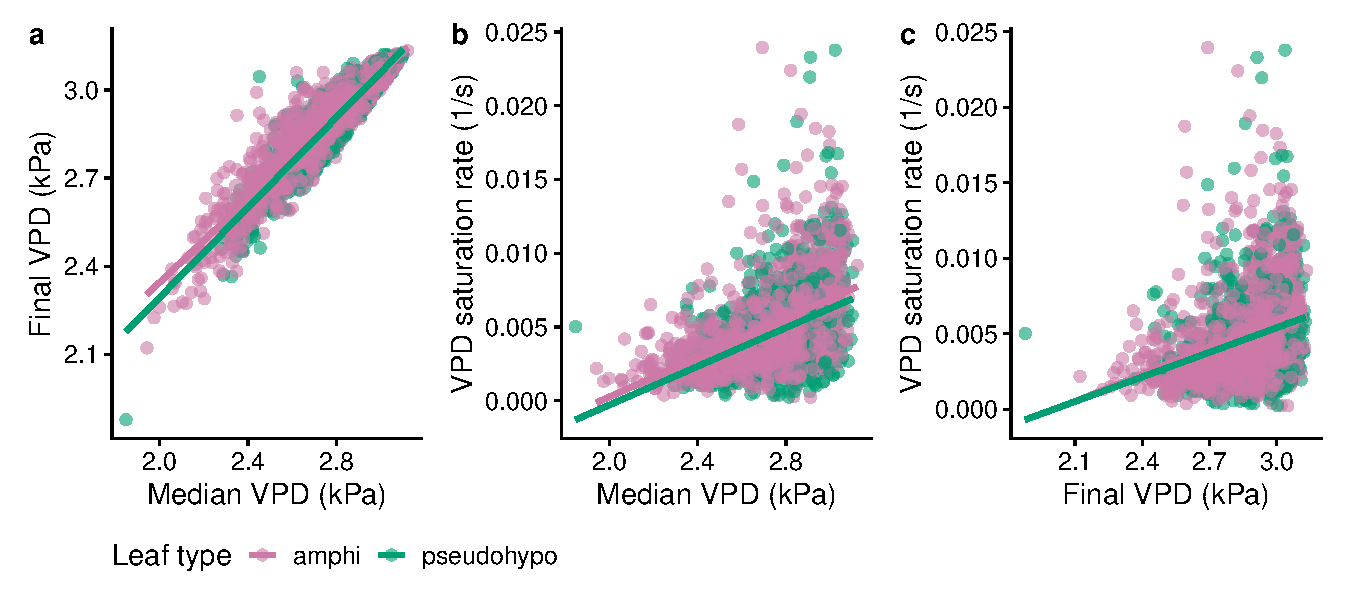
\includegraphics[keepaspectratio]{../figures/vpd-pairs.pdf}}

}
\DIFaddendFL 

\caption{\DIFdelbeginFL %DIFDELCMD < \label{fig-rh-curves}%%%
\DIFdelFL{Humidity-response curves and fitted lines}\DIFdelendFL \DIFaddbeginFL \label{fig-vpd-pairs}\textbf{\DIFaddFL{Pairwise relationships among curve-level VPD covariates.}}
\textbf{\DIFaddFL{a.}} \DIFaddFL{Median vs}\DIFaddendFL .\DIFdelbeginFL \DIFdelFL{The title provides }\DIFdelendFL \DIFaddbeginFL \DIFaddFL{~final VPD during }\DIFaddendFL the \DIFdelbeginFL \DIFdelFL{Tomato Genetics Resource Center accession number,
replicate letter, and species names}\DIFdelendFL \DIFaddbeginFL \DIFaddFL{fitted interval; }\textbf{\DIFaddFL{b.}}
\DIFaddFL{median VPD vs}\DIFaddendFL .\DIFdelbeginFL \DIFdelFL{The subtitle indicates the growth
light intensity (sun or shade)}\DIFdelendFL \DIFaddbeginFL \DIFaddFL{~VPD saturation rate \(k\); }\textbf{\DIFaddFL{c.}} \DIFaddFL{final VPD vs.~VPD
saturation rate \(k\). Each point is one humidity response curve}\DIFaddendFL ,
\DIFdelbeginFL \DIFdelFL{measurement light intensity (low or
high), and }\DIFdelendFL \DIFaddbeginFL \DIFaddFL{colored by }\DIFaddendFL leaf type\DIFdelbeginFL \DIFdelFL{(amphi or pseudohypo). Points are raw data and
}\DIFdelendFL \DIFaddbeginFL \DIFaddFL{; }\DIFaddendFL lines are \DIFdelbeginFL \DIFdelFL{fitted curves}\DIFdelendFL \DIFaddbeginFL \DIFaddFL{ordinary least-squares fits within leaf
type}\DIFaddendFL . \DIFdelbeginFL \DIFdelFL{The Bayesian correlation coefficient,
\(\mathrm{Bayes}~R^2\), }\DIFdelendFL \DIFaddbeginFL \DIFaddFL{VPD saturation rate }\DIFaddendFL is \DIFdelbeginFL \DIFdelFL{shown to }\DIFdelendFL the \DIFdelbeginFL \DIFdelFL{right }\DIFdelendFL \DIFaddbeginFL \DIFaddFL{rate constant }\DIFaddendFL of \DIFdelbeginFL \DIFdelFL{each curve}\DIFdelendFL \DIFaddbeginFL \DIFaddFL{a saturating
exponential fit to the VPD trajectory during the fitted interval (see
Notes S1)}\DIFaddendFL .}

\end{figure}%

\begin{figure}

\DIFaddbeginFL \centering{

\pandocbounded{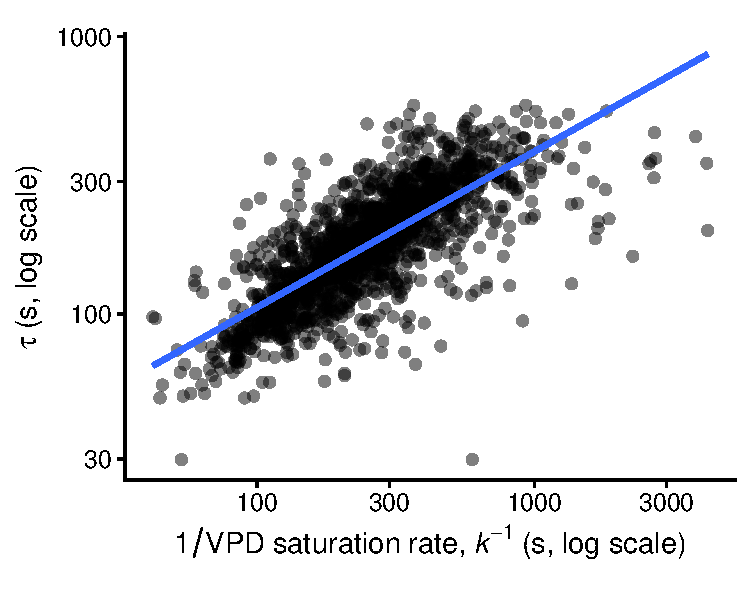
\includegraphics[keepaspectratio]{../figures/tau-vpd-rate.pdf}}

}

\caption{\label{fig-tau-vpd-rate}\textbf{\DIFaddFL{The stomatal closure time constant $\tau$ (log scale) is strongly correlated with the inverse of the VPD saturation rate $k^{-1}$ ($r = 0.77$ on log-log scale)}}\DIFaddFL{.
This is consistent with \(k\) being driven largely by the same
\gsw{{}}-decline signal that determines \(\tau\), rather than an
independent property of the VPD stimulus (see Notes S1). Each point is
one humidity response curve from the untreated (amphi) leaves. The blue
line us ordinary least-squares regression fit.}}

\end{figure}%DIF > 

\begin{figure}

\centering{

\pandocbounded{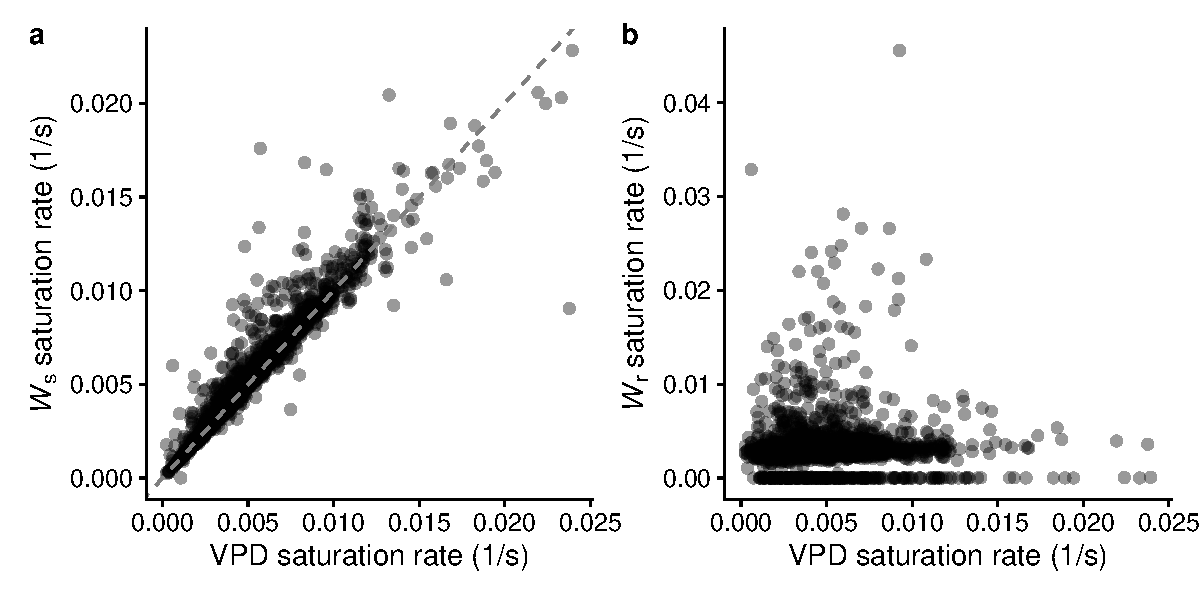
\includegraphics[keepaspectratio]{../figures/vpd-h2o-rate.pdf}}

}

\caption{\label{fig-vpd-h2o-rate}\textbf{\DIFaddFL{The VPD saturation rate is driven by the sample airstream, not the reference airstream.}}
\textbf{\DIFaddFL{a.}} \DIFaddFL{VPD saturation rate vs.~the saturation rate of
\(W_\mathrm{s}\) (sample cell water vapor concentration); the dashed
line is the 1:1 line. }\textbf{\DIFaddFL{b.}} \DIFaddFL{VPD saturation rate vs.~the saturation
rate of \(W_\mathrm{r}\) (reference cell water vapor concentration,
upstream of the leaf). Each point is one humidity response curve; rate
constants come from the same saturating-exponential model used for VPD.}}

\end{figure}%DIF > 

\begin{figure}

\centering{

\pandocbounded{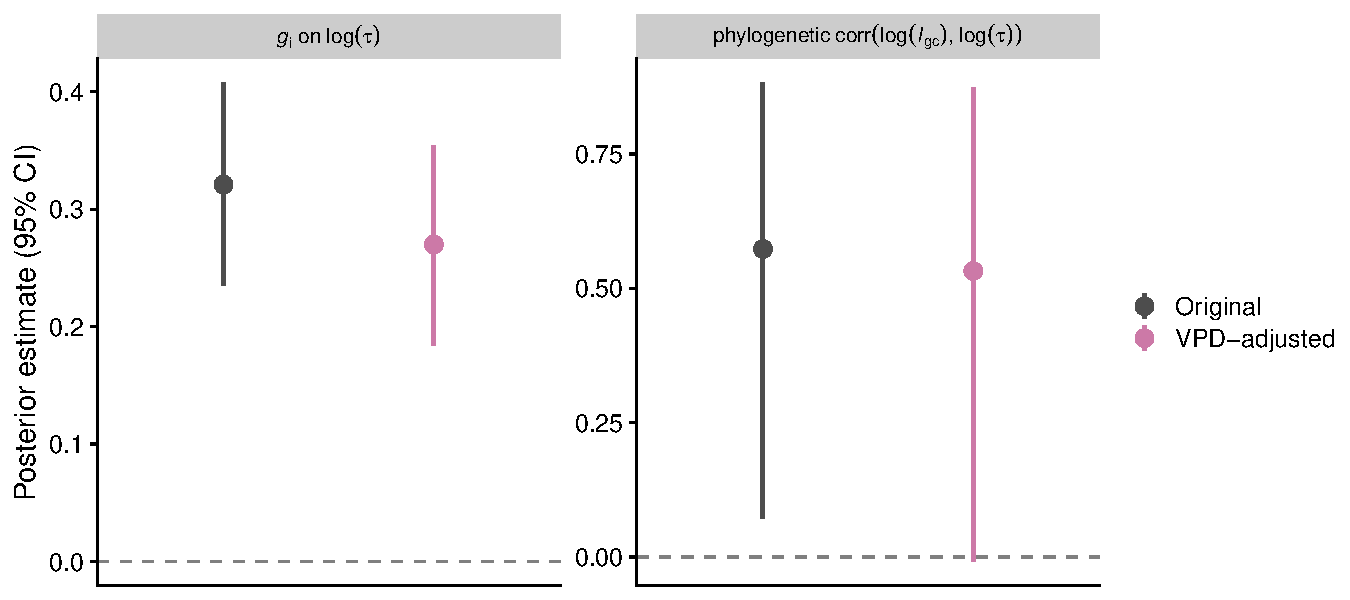
\includegraphics[keepaspectratio]{../figures/vpd-comparison.pdf}}

}

\caption{\label{fig-vpd-comparison}\textbf{\DIFaddFL{The \gi{} effect on $\tau$ and the phylogenetic correlation between \gcl{} and $\tau$ are robust to accounting for final VPD.}}
\DIFaddFL{Posterior means and 95\% credible intervals for the fixed effect of
\fgmax{} on \(\log \tau\) (left) and the phylogenetic correlation
between \(\log\) \gcl{} and \(\log \tau\) (right), comparing the
original model (grey) to a model refit with final VPD added as a
covariate of \(\tau\) and \(\lambda\) (pink; see Notes S1).}}

\end{figure}%DIF > 

\begin{figure}

\DIFaddendFL \centering{

\pandocbounded{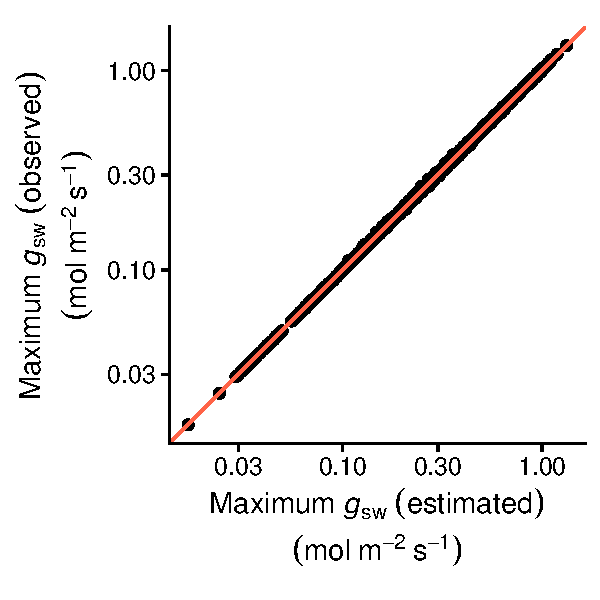
\includegraphics[keepaspectratio]{../figures/compare-gsw.pdf}}

}

\caption{\label{fig-compare-gsw}\textbf{The estimated ($x$-axis) and observed ($y$-axis) maximum stomatal conductances (\gsw) are nearly identical.}
Each point is the empirical maximum \gsw{} plotted against the estimated
\gsw{} for every humidity response curve. The orange line is the 1:1
line for reference. Both axes are on a log-scale.}

\end{figure}%

\begin{figure}

\DIFaddbeginFL \centering{

\textbf{Figure file:}\\
Download from:
\url{https://github.com/cdmuir/solanum-kinetics/raw/refs/heads/main/figures/rh-curves.pdf}

}

\caption{\label{fig-rh-curves}\textbf{\DIFaddFL{Humidity-response curves and
fitted lines.}} \DIFaddFL{The title provides the Tomato Genetics Resource Center
accession number, replicate letter, and species names. The subtitle
indicates the growth light intensity (sun or shade), measurement light
intensity (low or high), and leaf type (amphi or pseudohypo). Points are
raw data and lines are fitted curves. The Bayesian correlation
coefficient, \(\mathrm{Bayes}~R^2\), is shown to the right of each
curve.}}

\end{figure}%DIF > 

\begin{figure}

\DIFaddendFL \centering{

\pandocbounded{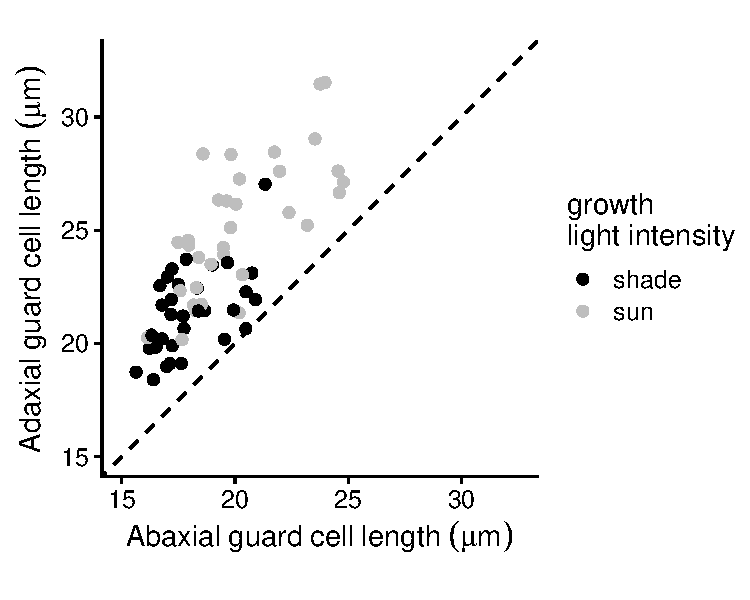
\includegraphics[keepaspectratio]{../figures/gcl.pdf}}

}

\caption{\label{fig-gcl}\textbf{Adaxial (upper) stomata are consistently larger than abaxial (lower) stomata in both sun-grown (grey points) and shade-grown (black points) plants.}
Each point was calculated by taking the median guard cell length within
each biological replicate and then calculating the mean among replicates
within each population and growth light intensity treatment. The dashed
line is the 1:1 line for reference. All points above this line indicate
larger values on the adaxial surface.}

\end{figure}%

\begin{figure}

\DIFdelbeginFL %DIFDELCMD < \centering{
%DIFDELCMD < 

%DIFDELCMD < \pandocbounded{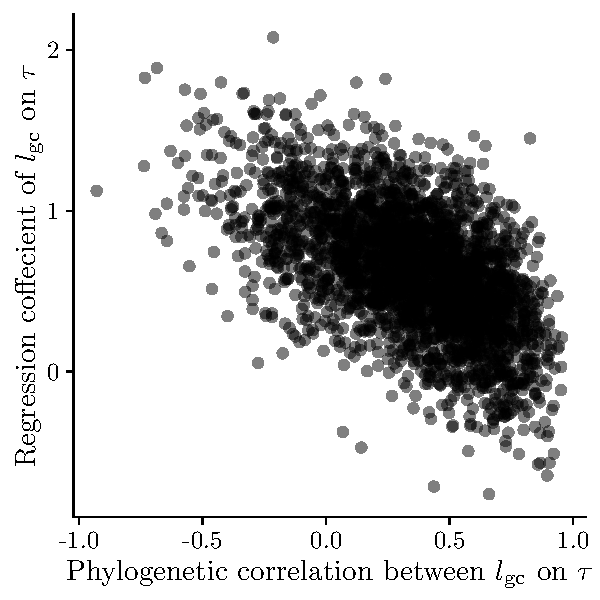
\includegraphics[keepaspectratio]{../figures/colinear.pdf}}
%DIFDELCMD < 

%DIFDELCMD < }
%DIFDELCMD < %%%
\DIFdelendFL \DIFaddbeginFL \centering{

\pandocbounded{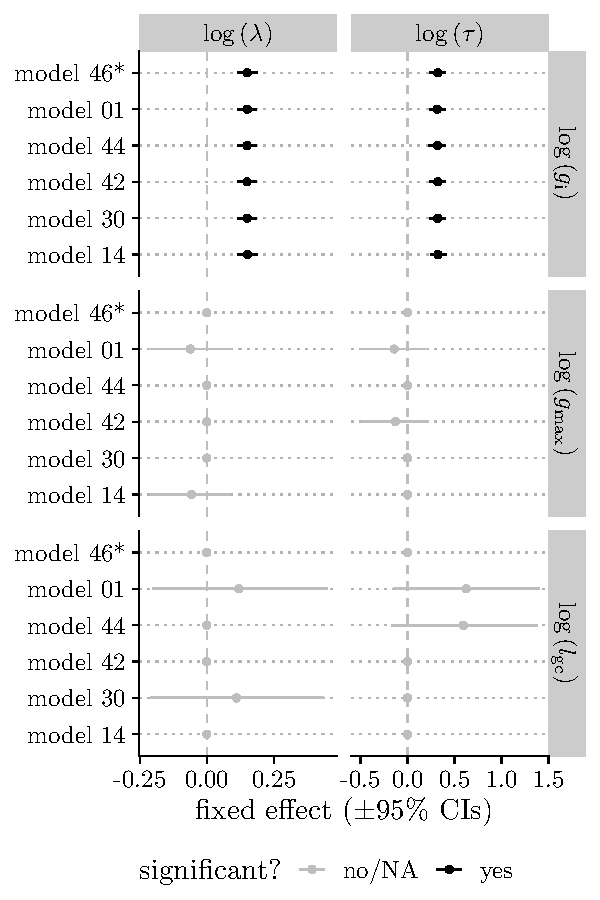
\includegraphics[keepaspectratio]{../figures/estimates-b.pdf}}

}
\DIFaddendFL 

\caption{\DIFdelbeginFL %DIFDELCMD < \label{fig-colinear}%%%
\textbf{\DIFdelFL{Posterior estimates of phylogenetic correlations ($x$-axis) and fixed effects ($y$-axis) of guard cell length (\gcl) on the time-constant ($\tau$) are colinear.}}
%DIFAUXCMD
\DIFdelFL{Each point is the estimate }\DIFdelendFL \DIFaddbeginFL \label{fig-estimates-b}\textbf{\DIFaddFL{Individual-level (fixed-effect) estimates of  initial stomatal conductance (\gi, top facets), anatomical maximum stomatal conductance (\gmax, middle facets), and guard cell length (\gcl, bottom facets) on the stomatal closure lag time ($\lambda$, left facets) and time constant ($\tau$, right facets) are broadly consistent across all plausible models.}}
\DIFaddFL{Points and horizontal bars are posterior medians and 95\% credible
intervals }\DIFaddendFL from \DIFdelbeginFL \DIFdelFL{one draw }\DIFdelendFL \DIFaddbeginFL \DIFaddFL{each }\DIFaddendFL of the \DIFdelbeginFL \DIFdelFL{posterior distribution
for both parameters from }\DIFdelendFL \DIFaddbeginFL \DIFaddFL{six plausible models (rows;
Table~\ref{tbl-comparison}), ordered by \(\Delta\)LOOIC; }\DIFaddendFL the \DIFaddbeginFL \DIFaddFL{selected
}\DIFaddendFL model \DIFaddbeginFL \DIFaddFL{is marked }\DIFaddendFL with \DIFdelbeginFL \DIFdelFL{the lowest LOOIC}\DIFdelendFL \DIFaddbeginFL \DIFaddFL{an asterisk (*)}\DIFaddendFL . \DIFdelbeginFL \DIFdelFL{The negative
relationship }\DIFdelendFL \DIFaddbeginFL \DIFaddFL{Black }\DIFaddendFL indicates \DIFaddbeginFL \DIFaddFL{estimates whose
95\% credible interval excludes zero; grey indicates intervals }\DIFaddendFL that
\DIFdelbeginFL \DIFdelFL{there is tradeoff in fitting the
relationship between variables as a higher level phylogenetic effect
versus a lower level, individual effect}\DIFdelendFL \DIFaddbeginFL \DIFaddFL{overlap zero}\DIFaddendFL .\DIFdelbeginFL \DIFdelFL{This results in more
uncertainty and larger confidence intervals in each individual
parameter.}\DIFdelendFL }

\end{figure}%

\begin{figure}

\DIFdelbeginFL %DIFDELCMD < \centering{
%DIFDELCMD < 

%DIFDELCMD < \pandocbounded{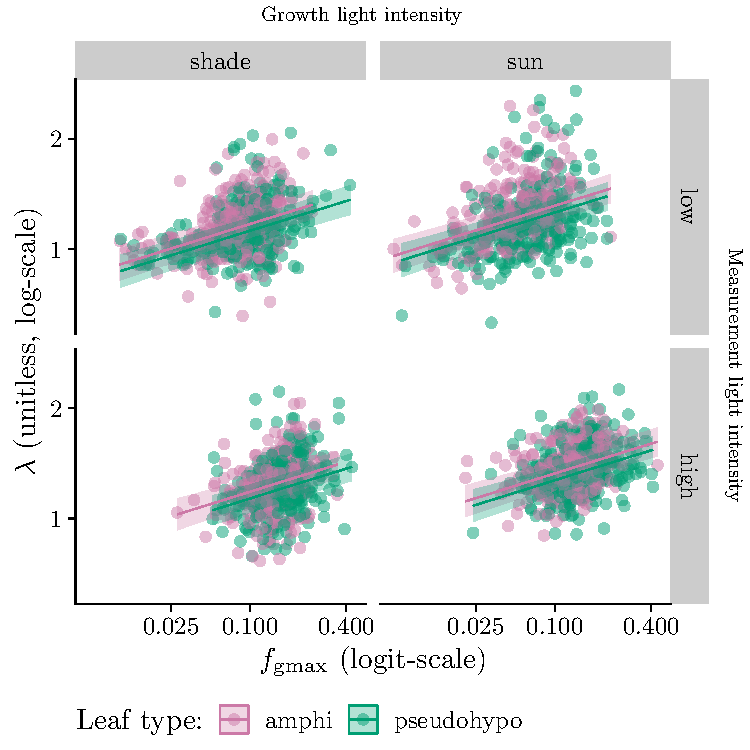
\includegraphics[keepaspectratio]{../figures/fgmax-lambda.pdf}}
%DIFDELCMD < 

%DIFDELCMD < }
%DIFDELCMD < %%%
\DIFdelendFL \DIFaddbeginFL \centering{

\pandocbounded{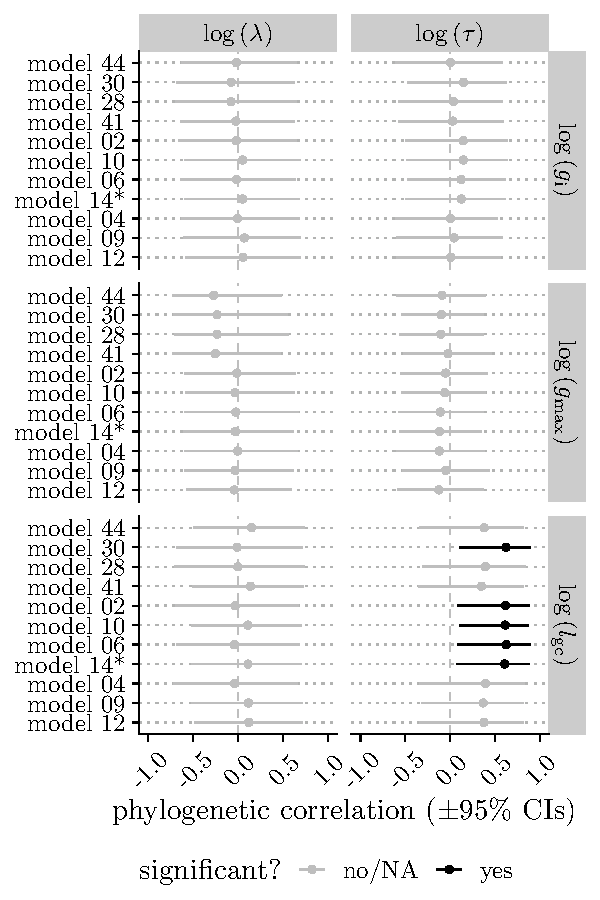
\includegraphics[keepaspectratio]{../figures/estimates-phy.pdf}}

}
\DIFaddendFL 

\caption{\DIFdelbeginFL %DIFDELCMD < \label{fig-fgmax-lambda}%%%
\textbf{\DIFdelFL{Individual-level variation in stomatal apertures influences stomatal closures kinetics.}}
%DIFAUXCMD
\DIFdelFL{As }\DIFdelendFL \DIFaddbeginFL \label{fig-estimates-phy}\textbf{\DIFaddFL{Phylogenetic correlations between initial stomatal conductance (\gi, top facets), anatomical maximum stomatal conductance (\gmax, middle facets), and guard cell length (\gcl, bottom facets) on the stomatal closure lag time ($\lambda$, left facets) and time constant ($\tau$, right facets) are broadly consistent across all plausible models.}}
\DIFaddFL{Points and horizontal bars are posterior medians and 95\% credible
intervals of }\DIFaddendFL the \DIFdelbeginFL \DIFdelFL{stomatal conductance as a fraction }\DIFdelendFL \DIFaddbeginFL \DIFaddFL{phylogenetic correlation from each }\DIFaddendFL of \DIFdelbeginFL \DIFdelFL{anatomical maximum stomatal
conductance }\DIFdelendFL \DIFaddbeginFL \DIFaddFL{the six plausible
models }\DIFaddendFL (\DIFdelbeginFL \DIFdelFL{\fgmax, \(x\)-axis}\DIFdelendFL \DIFaddbeginFL \DIFaddFL{rows; Table~\ref{tbl-comparison}}\DIFaddendFL )\DIFdelbeginFL \DIFdelFL{increases}\DIFdelendFL , \DIFaddbeginFL \DIFaddFL{ordered by \(\Delta\)LOOIC;
}\DIFaddendFL the \DIFdelbeginFL \DIFdelFL{stomatal closure
lag-time }\DIFdelendFL \DIFaddbeginFL \DIFaddFL{selected model is marked with an asterisk }\DIFaddendFL (\DIFdelbeginFL \DIFdelFL{\(\lambda\), \(y\)-axis}\DIFdelendFL \DIFaddbeginFL \DIFaddFL{*}\DIFaddendFL )\DIFdelbeginFL \DIFdelFL{increases}\DIFdelendFL . \DIFdelbeginFL \DIFdelFL{The overall pattern was
consistent across growth light intensity treatments (left }\DIFdelendFL \DIFaddbeginFL \DIFaddFL{Black indicates
estimates whose 95\% credible interval excludes zero; grey indicates
intervals that overlap zero.}}

\end{figure}%DIF > 

\begin{figure}

\centering{

\pandocbounded{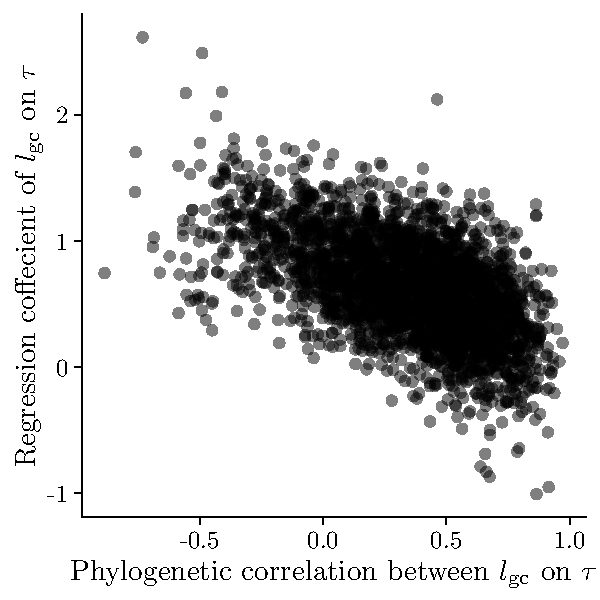
\includegraphics[keepaspectratio]{../figures/collinear.pdf}}

}

\caption{\label{fig-collinear}\textbf{\DIFaddFL{Posterior estimates of phylogenetic correlations ($x$-axis) and fixed effects ($y$-axis) of guard cell length (\gcl) on the time constant ($\tau$) are collinear.}}
\DIFaddFL{Each point is the estimate from one draw of the posterior distribution
for both parameters from the model with the lowest LOOIC. The negative
relationship indicates that there is tradeoff in fitting the
relationship between variables as a higher level phylogenetic effect
versus a lower level, individual effect. This results in more
uncertainty and larger confidence intervals in each individual
parameter.}}

\end{figure}%DIF > 

\begin{figure}

\centering{

\pandocbounded{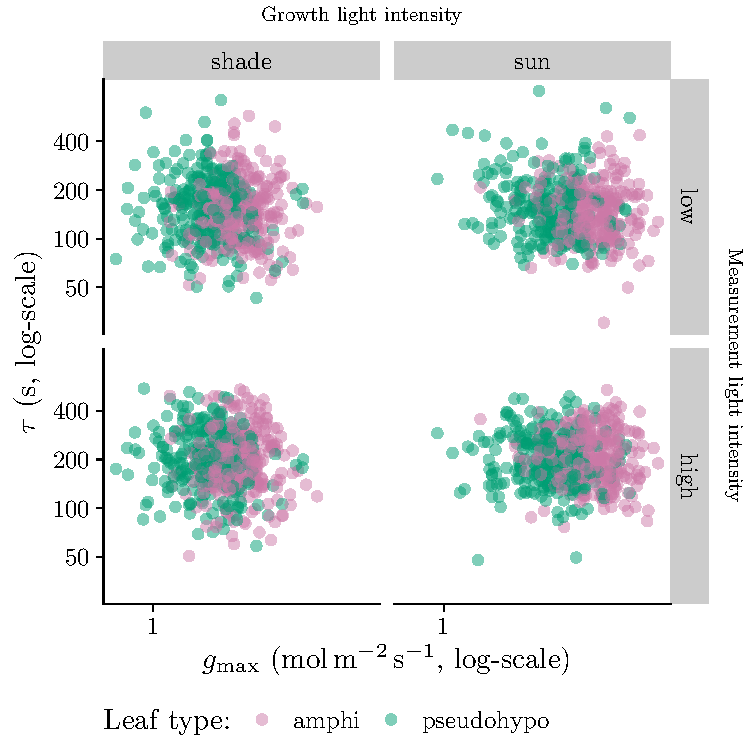
\includegraphics[keepaspectratio]{../figures/gmax-tau.pdf}}

}

\caption{\label{fig-gmax-tau}\textbf{\DIFaddFL{Individual-level variation in anatomical maximum stomatal conductance (\gmax) does not influence the stomatal closure time constant $\tau$.}}
\DIFaddFL{Individual-level variation in \gmax{} (\(x\)-axis) did not significantly
covary with \(\tau\) (\(y\)-axis). The overall pattern was consistent
across growth light intensity treatments (left and right facets),
measurement light intensity treatments (top and bottom facets), and leaf
types (point colors). The growth and measurement light intensity
treatments are described in the Materials and Methods section.}}

\end{figure}%DIF > 

\begin{figure}

\centering{

\pandocbounded{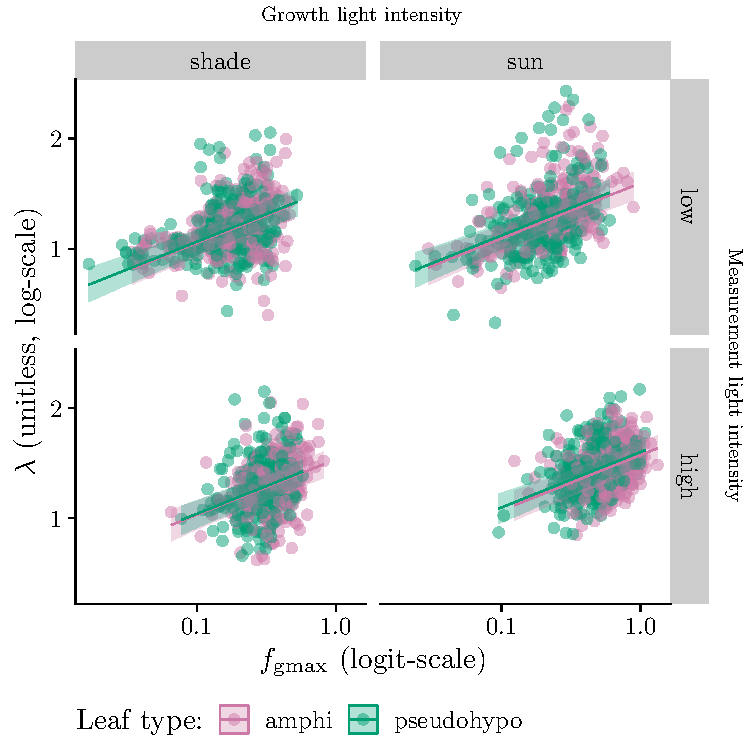
\includegraphics[keepaspectratio]{../figures/gi-lambda.pdf}}

}

\caption{\label{fig-gi-lambda}\textbf{\DIFaddFL{Individual-level variation in initial stomatal conductance (\gi) influences stomatal closure kinetics.}}
\DIFaddFL{As \gi{} (\(x\)-axis) increases, the stomatal closure lag time
(\(\lambda\), \(y\)-axis) increases. The overall pattern was consistent
across growth light intensity treatments (left and right facets),
measurement light intensity treatments (top and bottom facets), and leaf
types (point colors). Lines are estimated using linear regression along
with 95\% confidence ribbons. The growth and measurement light intensity
treatments are described in the Materials and Methods section.}}

\end{figure}%DIF > 

\begin{figure}

\centering{

\pandocbounded{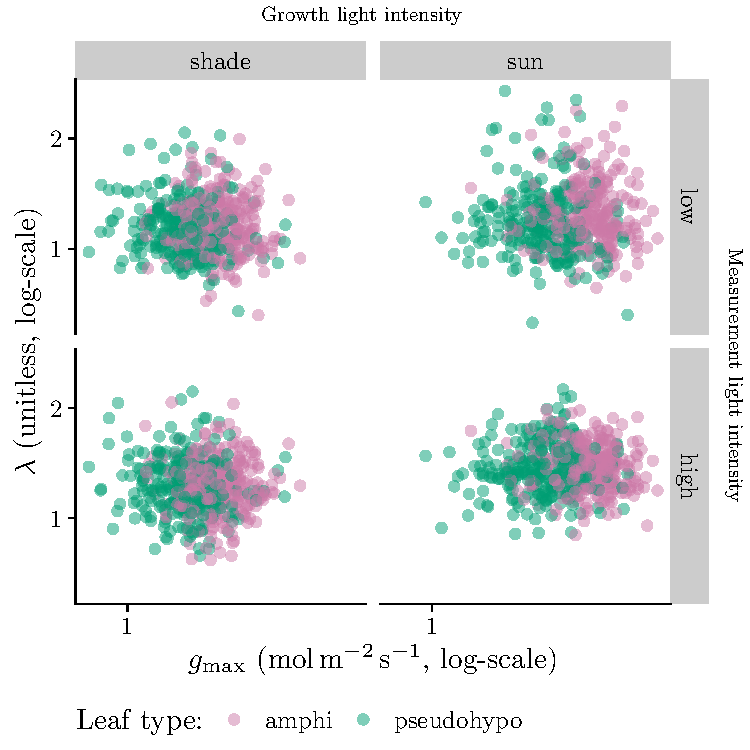
\includegraphics[keepaspectratio]{../figures/gmax-lambda.pdf}}

}

\caption{\label{fig-gmax-lambda}\textbf{\DIFaddFL{Individual-level variation in anatomical maximum stomatal conductance (\gmax) does not influence the stomatal closure lag time $\lambda$.}}
\DIFaddFL{Individual-level variation in \gmax{} (\(x\)-axis) did not significantly
covary with \(\lambda\) (\(y\)-axis). The overall pattern was consistent
across growth light intensity treatments (left and right facets),
measurement light intensity treatments (top and bottom facets), and leaf
types (point colors). The growth and measurement light intensity
treatments are described in the Materials and Methods section.}}

\end{figure}%DIF > 

\clearpage

\newpage{}

\subsection{\DIFadd{Supporting notes}}\label{supporting-notes}

\subsubsection{\texorpdfstring{Notes S1: Effects of \gi{} and \gcl{} are
robust to variation in VPD
stimulus}{Notes S1: Effects of  and  are robust to variation in VPD stimulus}}\label{notes-s1-effects-of-and-are-robust-to-variation-in-vpd-stimulus}

\DIFadd{Table~\ref{tbl-vpd} shows that the mean VPD realized during measurements
differed among treatment combinations
(\(\SI{2.72}{\kPa}\)--\(\SI{3}{\kPa}\)), because leaf transpiration
itself humidifies the chamber and \gsw{} varied systematically with
measurement light, growth light, and leaf type. Because VPD is the
physiological driver of stomatal closure, we checked whether this
variation in the realized stimulus could confound the effects of \gi{}
and \gcl{} on the closure time constant, \(\tau\).
}

\DIFadd{For every curve we extracted the leaf-to-air VPD trajectory from the
logged humidity data and derived two curve-level covariates: final VPD
and VPD saturation rate (\(k\)). Final VPD is the VPD at the end of the
fitted interval; \(k\) is the rate constant of a saturating exponential,
\(\mathrm{VPD}(t) = B + (R_0 - B)\exp(-kt)\), fit separately to each
curve (median \(R^2 = 0.99\), \(n = 2,156\) curves; \(k\) excluded for
15 curves with a poor saturating fit or an extreme outlier rate
estimate). We also considered median VPD. Median and final VPD were
highly correlated (\(r = 0.93\); Figure~\ref{fig-vpd-pairs}a), so we
retained only final VPD.
}

\DIFadd{We did not include the VPD saturation rate as a covariate of \(\tau\),
because \(k\) }\DIFaddend and \DIFdelbegin \DIFdel{right
facets)}\DIFdelend \DIFaddbegin \DIFadd{\(\tau\) are themselves strongly correlated
(\(r = 0.77\); Figure~\ref{fig-tau-vpd-rate}) for a mechanistic rather
than confounding reason: the VPD trajectory during the analyzed interval
is driven mainly by declining leaf transpiration as stomata close, so
\(k\) largely tracks the same \gsw{}-decline signal that determines
\(\tau\). We tested this by fitting the same saturating-exponential
model to the sample-cell water vapor concentration (\(W_\mathrm{s}\))
and the reference-cell water vapor concentration (\(W_\mathrm{r}\),
upstream of the leaf and largely reflecting the controlled incoming
airstream). The VPD saturation rate closely tracked the \(W_\mathrm{s}\)
saturation rate (\(r = 0.95\)) but not the \(W_\mathrm{r}\) saturation
rate (\(r = 0.02\)) (Figure~\ref{fig-vpd-h2o-rate}). Including \(k\) as
a covariate of \(\tau\) would therefore be close to circular.
}

\DIFadd{To directly test whether the realized VPD stimulus confounds the \gi{}
and \gcl{} effects on \(\tau\), we refit the selected model with final
VPD added as a covariate of \(\tau\) and \(\lambda\)
(Figure~\ref{fig-vpd-comparison}). The individual-level effect of \gi{}
on \(\log \left( \tau \right)\) was slightly weaker (original: 0.32
}{[}\DIFadd{0.23}\DIFaddend , \DIFdelbegin \DIFdel{measurement light intensity treatments }\DIFdelend \DIFaddbegin \DIFadd{0.41}{]}\DIFadd{; VPD-adjusted: 0.27 }{[}\DIFadd{0.18, 0.36}{]}\DIFadd{), as was the
phylogenetic correlation between \gcl{} and \(\tau\) (original: 0.59
}{[}\DIFadd{0.14, 0.88}{]}\DIFadd{; VPD-adjusted: 0.54 }{[}\DIFadd{-0.04, 0.88}{]}\DIFadd{). This indicates
that variation in VPD slightly amplified the apparent effects of \gi{}
and \gcl{} on stomatal closure kinetics, but does not qualitatively
change the main conclusions. Final VPD itself had a negative fixed
effect on \(\log \left( \tau \right)\) }\DIFaddend (\DIFdelbegin \DIFdel{top }\DIFdelend \DIFaddbegin \DIFadd{-0.41 }{[}\DIFadd{-0.53, -0.27}{]}\DIFadd{),
consistent with higher realized VPD accelerating stomatal closure.
}

\DIFadd{We lack data on the rate of VPD change during the wrong-way response and
the earliest part of the right-way response, because humidity logging
did not begin until \gsw{} had already declined back to its pre-step
value (Figure~\ref{fig-conceptual}a); this limits our ability to
evaluate whether the }\emph{\DIFadd{initial}} \DIFadd{rate of VPD change, as opposed to
the final realized VPD, influenced closure kinetics. We recommend that
future studies of stomatal kinetics log chamber humidity continuously
from the onset of the humidity step to more fully characterize the
realized VPD stimulus and adjust the incoming airstream to keep VPD
constant as stomatal close.
}

\newpage{}

\subsubsection{\texorpdfstring{Notes S2: The \gi{}-\(\tau\) association
is not an artifact of the curve-fitting
procedure}{Notes S2: The -\textbackslash tau association is not an artifact of the curve-fitting procedure}}\label{notes-s2-the--tau-association-is-not-an-artifact-of-the-curve-fitting-procedure}

\DIFadd{The initial conductance \gi{} used to calculate \fgmax{} is estimated
from the same nonlinear fit (Equation~\ref{eq-weibull}) that also
estimates \(\tau\) }\DIFaddend and \DIFdelbegin \DIFdel{bottom facets}\DIFdelend \DIFaddbegin \DIFadd{\(\lambda\) for each curve. This raises the
possibility that parameter covariance within the curve fit itself,
rather than a true biological relationship, could generate an
association between \gi{} and \(\tau\) (and hence \fgmax{} and \(\tau\),
since the denominator \(g_\mathrm{max}\) is estimated independently from
stomatal anatomy and cannot itself introduce a fitting artifact). To
test this, we ran a null simulation in which any true association
between \gi/\gf{} and the kinetic parameters was removed by
construction. For every real curve \(i\), we simulated a synthetic
\gsw{} trajectory using curve \(i\)'s own measurement times, residual
noise magnitude, and fitted \(\tau\) and \(\lambda\), but with \gi{} and
\gf{} taken from a different, randomly chosen curve \(j\). Because \(i\)
and \(j\) were chosen independently at random, the synthetic curves
retain realistic variability in both \(\tau\)/\(\lambda\) and \gi/\gf,
but there is no true association between \gi{} and the kinetic
parameters. We re-fit the same Weibull functional form to each synthetic
curve using nonlinear least squares (}\texttt{\DIFadd{nls()}}\DIFadd{), which closely
approximated the full Bayesian pipeline used for the real data when
compared directly on the real curves (cor(\(\tau\)}\DIFaddend ) \DIFaddbegin \DIFadd{= 0.99,
cor(\(\lambda\)) = 1.00), and computed the correlation between the
}\emph{\DIFadd{estimated}} \DIFadd{\gi{} and \(\log(\tau)\). We repeated this 1}\DIFaddend ,\DIFdelbegin \DIFdel{and leaf types }\DIFdelend \DIFaddbegin \DIFadd{000 times
to build a null distribution of this correlation.
}

\DIFadd{The null-simulation correlations ranged from -0.06 to 0.09 (median
\(-3.1 \times 10^{-3}\)) across the 1,000 replicates, indistinguishable
from zero (Figure~\ref{fig-null-sim-fgmax-tau}). In contrast, the real,
observed correlation between \gi{} and \(\log(\tau)\) is 0.39 }{[}\DIFadd{0.35,
0.42}{]}\DIFadd{, far outside the null range (empirical \(p\) = 0.000). This
indicates that the curve-fitting procedure alone cannot explain the
observed \gi{}-\(\tau\) association, supporting our interpretation that
it reflects a real relationship in the data rather than a statistical
artifact of estimating \gi, \(\tau\), and \(\lambda\) from the same
nonlinear fit.
}

\begin{figure}

\centering{

\pandocbounded{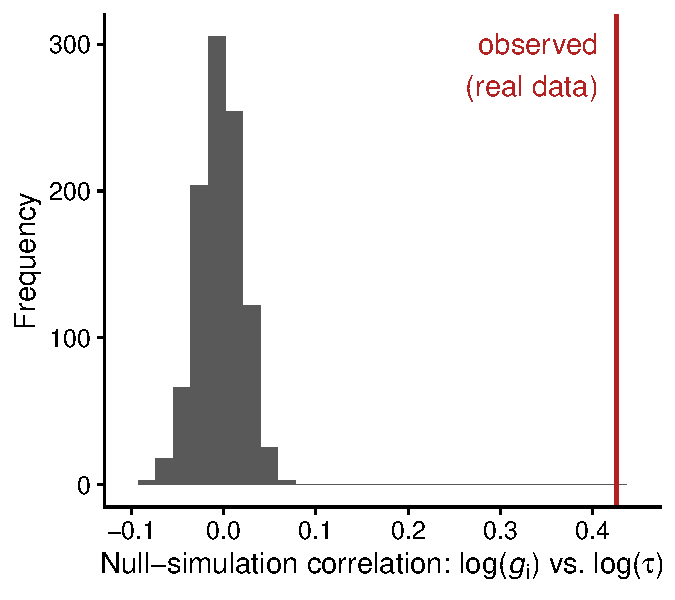
\includegraphics[keepaspectratio]{../figures/null-sim-fgmax-tau.pdf}}

}

\caption{\label{fig-null-sim-fgmax-tau}\textbf{\DIFaddFL{The curve-fitting procedure alone does not induce a $g_\mathrm{i}$-$\tau$ association.}}
\DIFaddFL{Null distribution of the correlation between estimated \gi{} and
estimated \(\tau\) across 1,000 simulated datasets in which the true
\gi{} and \gf{} are fixed at their real median values for every curve
(so \gi{} has no true relationship with \(\tau\) by construction),
compared to the observed correlation in the real data (red line).}}

\end{figure}%DIF > 

\newpage{}

\subsubsection{\texorpdfstring{Notes S3: Sensitivity analysis of the
\gi{}-\(\tau\) path analysis to unmeasured
confounding}{Notes S3: Sensitivity analysis of the -\textbackslash tau path analysis to unmeasured confounding}}\label{notes-s3-sensitivity-analysis-of-the--tau-path-analysis-to-unmeasured-confounding}

\DIFadd{The path analysis linking treatment, \gi{}, and \(\tau\) assumes the
causal structure in Figure~\ref{fig-mediation-dag}: each treatment has a
direct effect on \(\tau\) and an indirect effect acting through \gi{}.
This structure is only identified as causal under sequential
ignorability, i.e., that no unmeasured confounder \(U\) (e.g., hydraulic
status, measurement order, realized VPD trajectory) affects both \gi{}
and \(\tau\). If such a \(U\) exists (dashed arrows), the correlation it
induces between the \gi{} and \(\tau\) equations' residuals is exactly
the sensitivity parameter \(\rho\) examined below.
}

\begin{figure}

\centering{

\pandocbounded{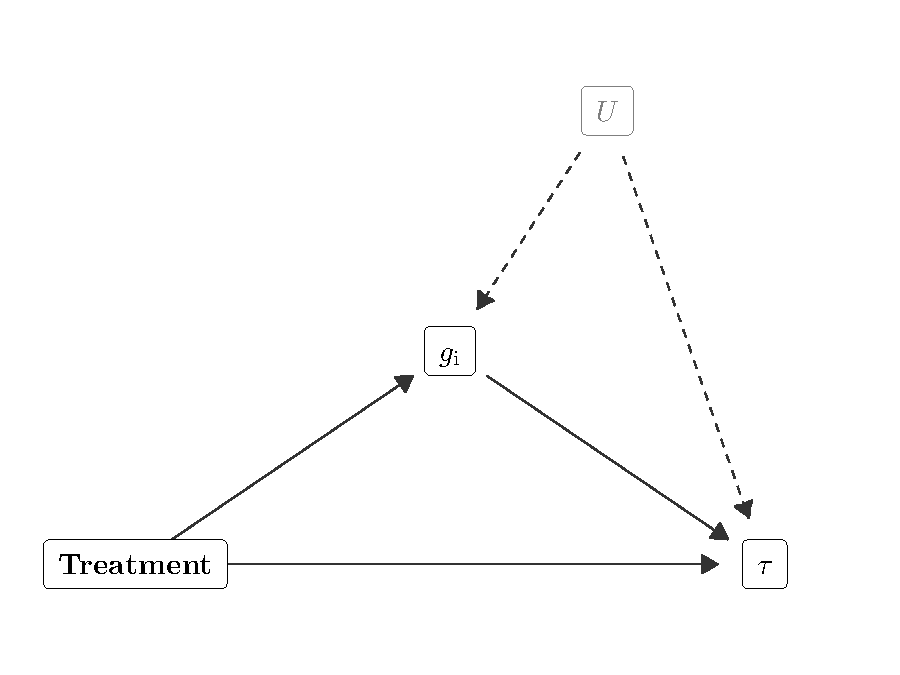
\includegraphics[keepaspectratio]{../figures/mediation-dag.pdf}}

}

\caption{\label{fig-mediation-dag}\textbf{\DIFaddFL{Assumed causal structure of the \gi{}-$\tau$ path analysis.}}
\DIFaddFL{Treatment has a direct effect on \(\tau\) (bottom arrow) and an indirect
effect acting through \gi{} (upper path). An unmeasured confounder \(U\)
(dashed arrows) affecting both \gi{} and \(\tau\) -- e.g., hydraulic
status, measurement order, or realized VPD trajectory -- would violate
the sequential ignorability assumption required to interpret the
indirect path causally.}}

\end{figure}%DIF > 

\DIFadd{The path analysis linking \gi{} to \(\tau\) (see Materials and Methods,
``Path analysis to test for plastic effects'') assumes sequential
ignorability: that there is no unmeasured confounder of the
\gi{}-\(\tau\) relationship after conditioning on treatment and the
random effects already in the model. Because \gi{} is not randomized, is
estimated from the same curve as \(\tau\), and could share unmeasured
confounders (e.g., hydraulic status, measurement order, realized VPD
trajectory) with \(\tau\), we assessed this assumption directly with a
sensitivity analysis following the general framework of Imai }\emph{\DIFadd{et
al.}} \DIFaddend (\DIFdelbegin \DIFdel{point colors)}\DIFdelend \DIFaddbegin \DIFadd{2010), parameterized by
\(\rho = \mathrm{Cor}(e_{g_\mathrm{i}}, e_\tau)\), the residual
correlation between the \gi{} and \(\tau\) equations. Under a violation
of sequential ignorability with residual correlation \(\rho\), the
bias-adjusted mediator-on-outcome coefficient is
\(\beta_2(\rho) = \hat\beta_2 - \rho \cdot \sigma_\tau / \sigma_{g_\mathrm{i}}\),
so the indirect effect of a treatment acting through \gi{} is
\(\gamma_1 \cdot \beta_2(\rho)\) (where \(\gamma_1\) is the effect of
treatment on \gi), and the ``breakdown point'' \(\rho^*\) at which this
indirect effect is exactly zero is
\(\rho^* = \hat\beta_2 \cdot \sigma_{g_\mathrm{i}} / \sigma_\tau\)}\DIFaddend .
\DIFdelbegin \DIFdel{Lines are estimated using linear
regression along with 95\% confidence ribbons}\DIFdelend \DIFaddbegin 

\DIFadd{Our selected model already estimates a free residual correlation between
the \gi{} and \(\tau\) equations, because we fit all five responses
(\gcl, \gi, \gmax, \(\tau\), \(\lambda\)) jointly. Because the \gi{}
equation's predictors are a strict subset of \(\tau\)'s, jointly
estimating this correlation does not change the point estimate of
\(\hat\beta_2\) relative to a model that assumes \(\rho = 0\) (a
standard result for seemingly unrelated regression models), so we can
treat \(\hat\beta_2\) as the ``naive'' coefficient in the sensitivity
framework above, and the model's own estimated residual correlation as a
data-driven estimate of \(\rho\)}\DIFaddend .
\DIFdelbegin \DIFdel{The growth }\DIFdelend \DIFaddbegin 

\DIFadd{We found \(\rho_\mathrm{estimated}\) = 0.06 }{[}\DIFadd{-0.07, 0.18}{]} \DIFaddend and
\DIFdelbegin \DIFdel{measurement light intensity treatments are described in the Materials
and Methods section.}%DIFDELCMD < \MBLOCKRIGHTBRACE
%DIFDELCMD < %%%
\DIFdelend \DIFaddbegin \DIFadd{\(\rho^*\) = 0.40 }{[}\DIFadd{0.29, 0.51}{]}
\DIFadd{(Figure~\ref{fig-mediation-sensitivity}). These posterior distributions
do not substantially overlap and the posterior probability that the
estimated residual correlation is smaller in magnitude than the
breakdown point is nearly 100\%. In other words, the plastic mediation
effects of \gi{} on \(\tau\) are probably not explained by unmeasured
confounders.
}

\begin{figure}

\centering{

\pandocbounded{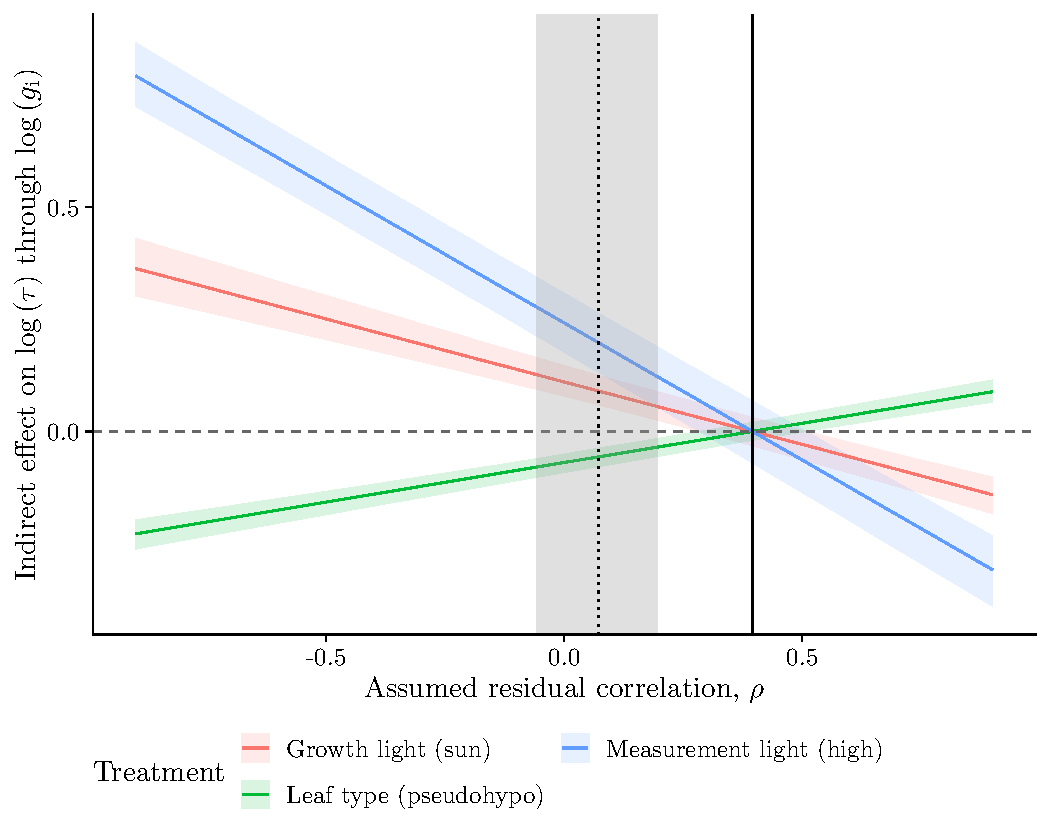
\includegraphics[keepaspectratio]{../figures/mediation-sensitivity.pdf}}

}

\caption{\label{fig-mediation-sensitivity}\textbf{\DIFaddFL{Sensitivity of the indirect effect of each treatment on $\log \tau$, acting through \gi, to an assumed residual correlation $\rho$ between the \gi{} and $\tau$ equations.}}
\DIFaddFL{The vertical dotted line is the model's own estimated residual
correlation (\(\rho_\mathrm{estimated}\), shaded band = 95\% credible
interval); the vertical solid line is the breakdown point \(\rho^*\) at
which the indirect effect is zero.}}
\DIFaddendFL 

\end{figure}%




\end{document}
